\chapter{METODOLOGI PENELITIAN}
\label{chap:chap3_metodologi}

\section*{}
Pada penelitian ini nantinya akan terdiri dari lima langkah utama yaitu analisa komponen permainan RPG, desain level dan \textit{stats} atau atribut gameplay pada karakter pemain, desain level dan \textit{stats} pada setiap karakter musuh, dilanjutkan pengujian hasil \textit{stats} pada karakter pemain dan musuh, kemudian dilakukan klasifikasi dengan \textit{Neural Network Mullticlass Classification}. Setiap langkah yang dilakukan dibawahnya merupakan detail dalam pengerjaan seperti yang direpresentasikan pada Gambar \ref{fig:metodologi}.
\vspace{1ex}

\begin{figure} [!h] \centering
	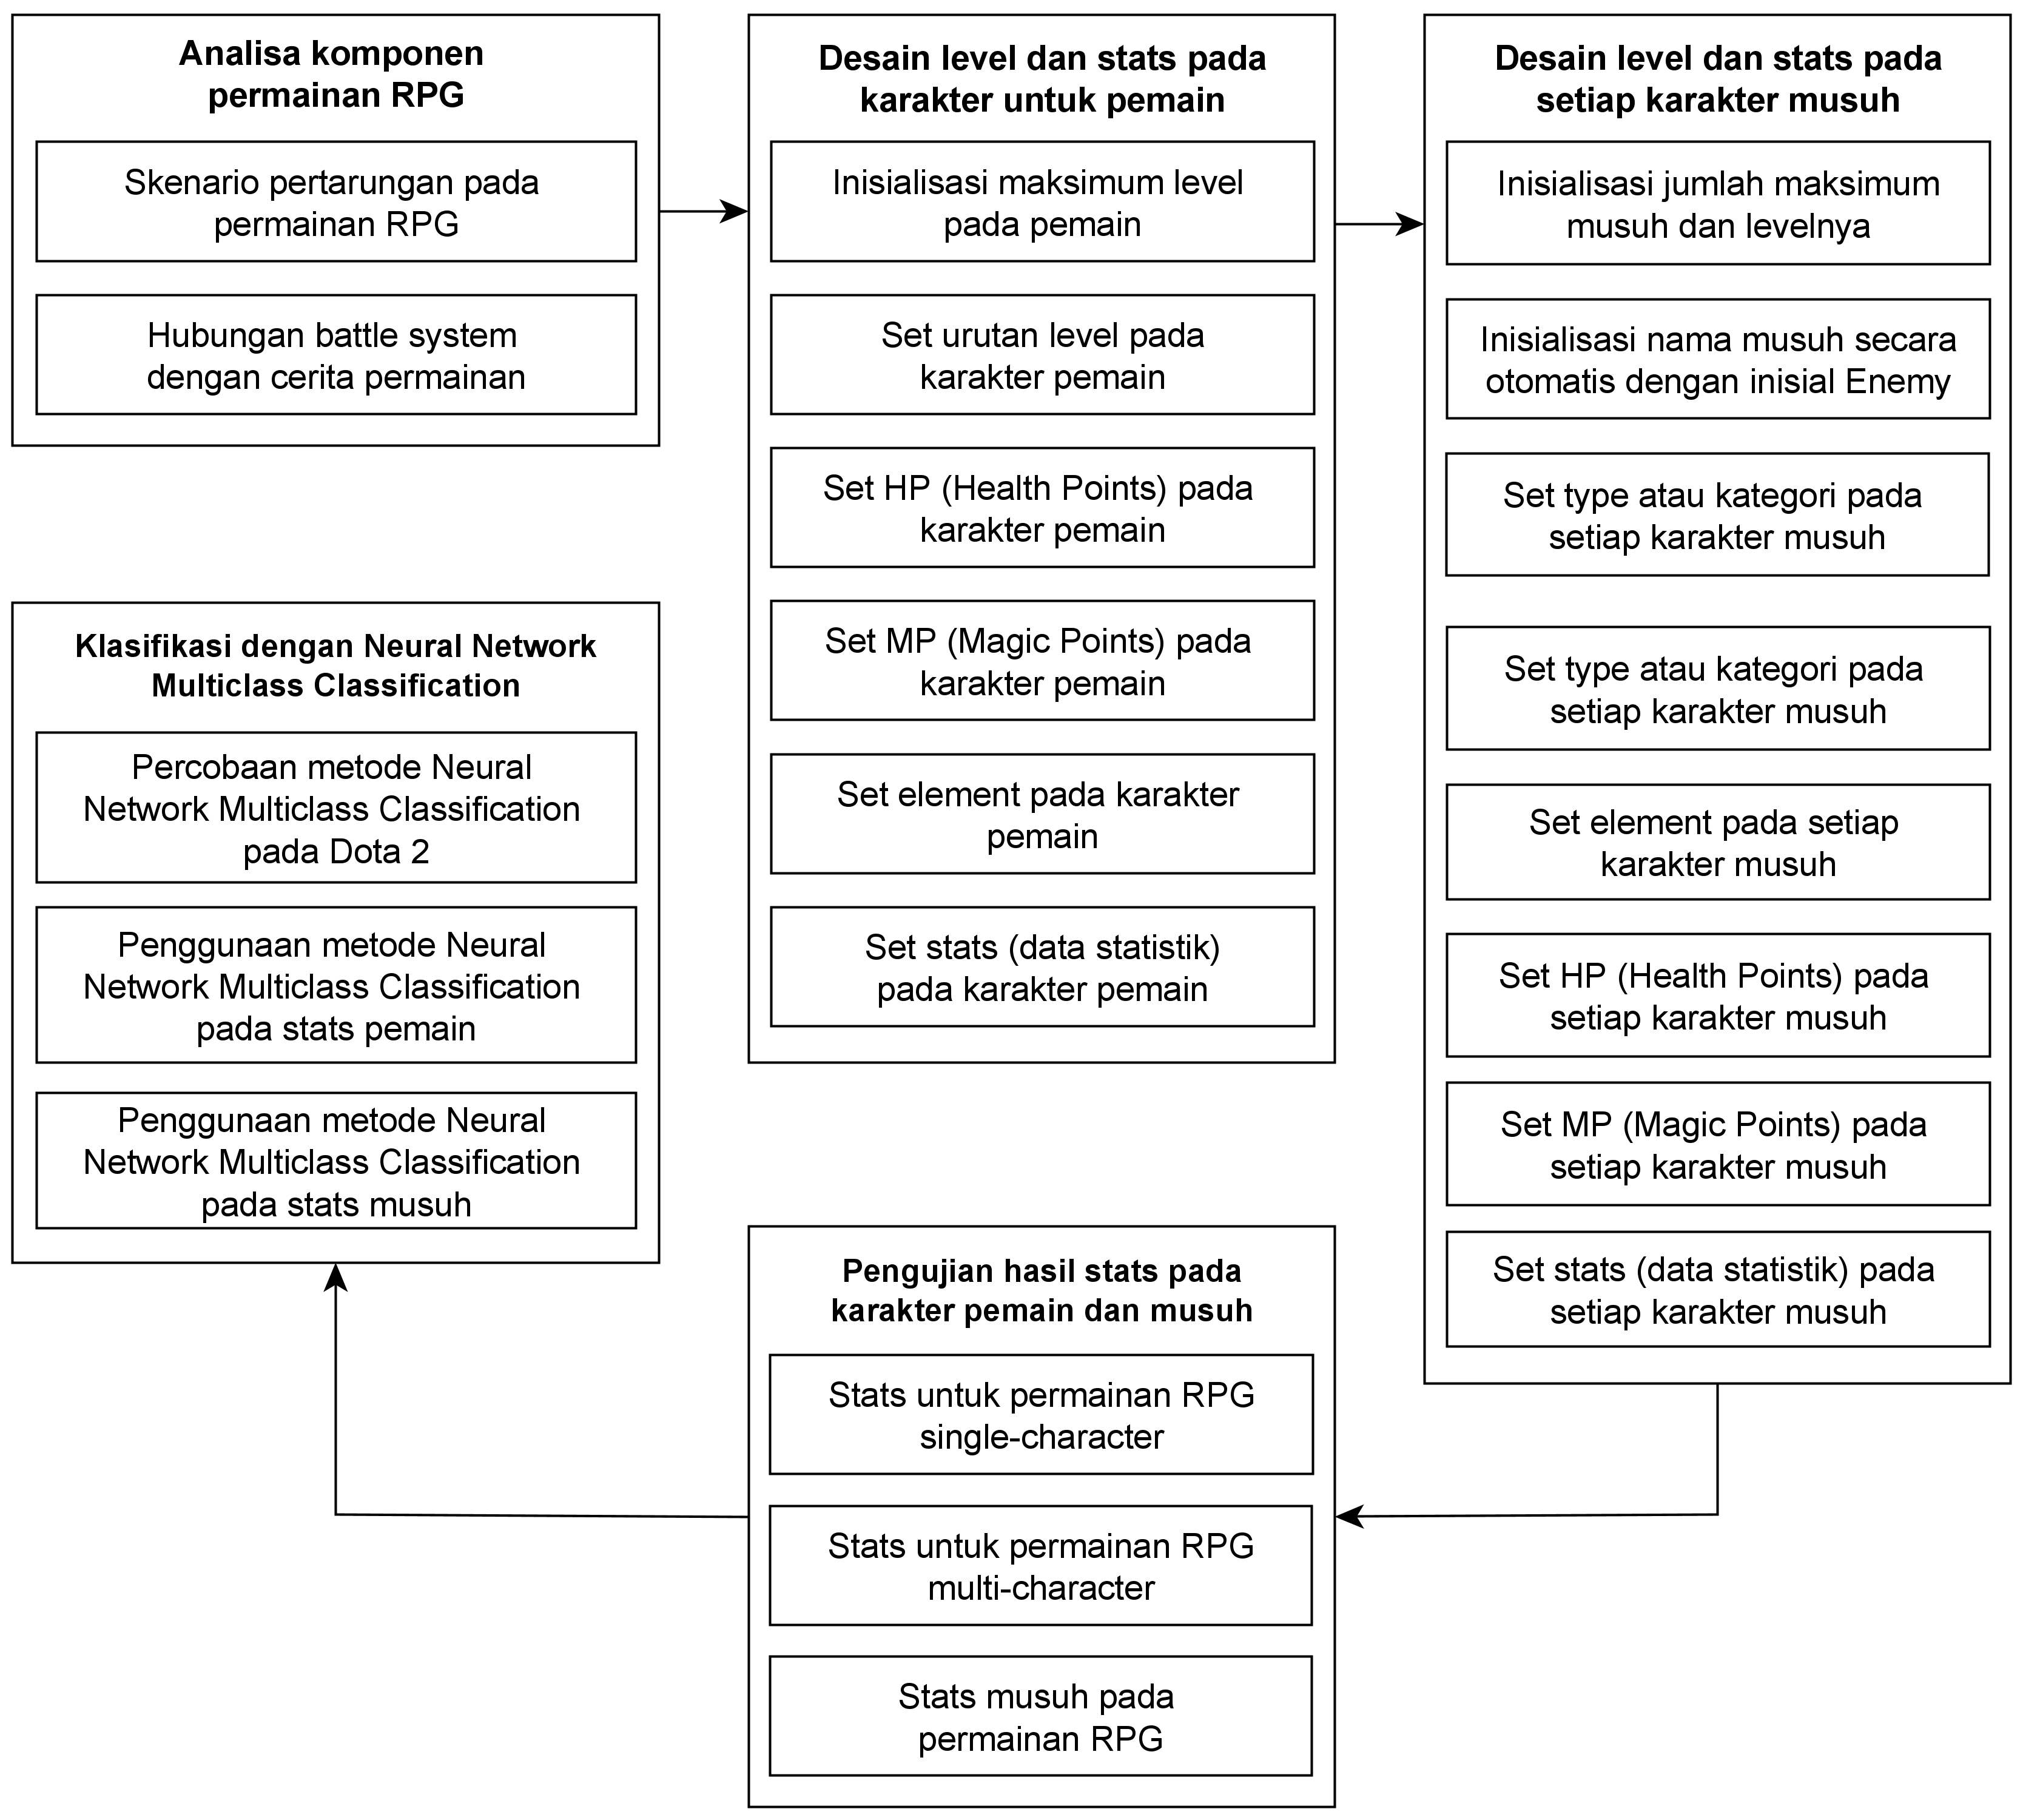
\includegraphics[scale=0.12]{img/metodologi_5.png}
	\caption{Urutan metodologi.}
	\label{fig:metodologi}
\end{figure}
\vspace{1ex}

Tujuan umum dari penelitian ini adalah membuat \textit{stats} atau statistik untuk pemain dan musuh, sehingga dalam pembuatan permaian. Tujuan khusus dan fokus pada penelitian ini adalah untuk membuat \textit{stats} untuk karakter pemain dan musuh dengan menggunakan metode $k-$NN dan \textit{Naive Bayes} yang kemudian dilakukan klasifikasi dengan menggunakan metode \textit{Neural Network} \textit{Multiclass Classification}.
\vspace{1ex}

\section{Analisa Komponen Permainan RPG}
\label{sec:sec3_design_komponen}
\vspace{1ex}

Pada bagian ini terdapat beberapa langkah yang akan menjelaskan penyusunan skenario pertarungan pada permainan RPG \textit{turn-based}. Pertama yang akan dilakukan adalah pembuatan skenario pertarungan pada permainan \textit{turn-based} RPG. Dari skenario tersebut tentunya harus ada hubungan dengan cerita dari permainan, apa saja parameter yang berpengaruh dari cerita terhadap skenario. Dalam proses analisa ini cukup dilakukan pada RPG yang tergolong \textit{turn-based}, karena hal tersebut dianggap paling ideal. Saat karakter pemain dan musuh saling serang secara bergantian.
\vspace{1ex}

Di lanjutkan dengan desain level dan \textit{stats} dari pemain, selain itu digunakannya algoritma $k-$NN (\textit{Nearest Neighbor}) untuk mempercepat proses pembuatannya. Kemudian dilanjutkan dengan desain level dan \textit{stats} musuh yang juga dibuat secara otomatis dengan algoritma yang sama dengan pemain, namun tetap dipolakan oleh \textit{gaussian naive bayes} atau distribusi normal. 
\vspace{1ex}

Bagian selanjutnya adalah penambahan elemen pada pemain dan musuh yang membentuk kelebihan atau kekurangan pada masing-masing karakter. Pembagian elemen pada karakter yang dapat dimainkan oleh pemain dilakukan sesuai dengan cerita, sedangkan pembagian elemen pada musuh disebar secara acak berdasarkan \textit{stats} yang telah dibuat. Hal ini berkaitan erat dengan penjelasan pada Sub-bab \ref{sec:sub_sec2_kesempatan} tentang meningkatnya keberagaman, yang dibuktikan dengan banyaknya variasi musuh berikut dengan kelemahan dan kelebihannya.
\vspace{1ex}

\subsection{Desain Skenario Pertarungan}
\label{sec:sub_sec3_design_skenario}
\vspace{1ex}

Di umpamakan jumlah karakter yang rencananya akan digunakan berjumlah tunggal atau \textit{single-character} (WRPG, ARPG, SRPG, dan MMORPG) sampai tiga karakter atau jamak atau \textit{multi-character} (TRPG dan JRPG) bergantung dengan alur cerita dari permainan dan jumlah musuh juga dimisalkan berjumlah antara satu sampai dengan enam, bergantung kepada tingkat kesulitannya seperti pada Gambar \ref{fig:battle_player}. 
\vspace{1ex}

\begin{figure} [!h] \centering
	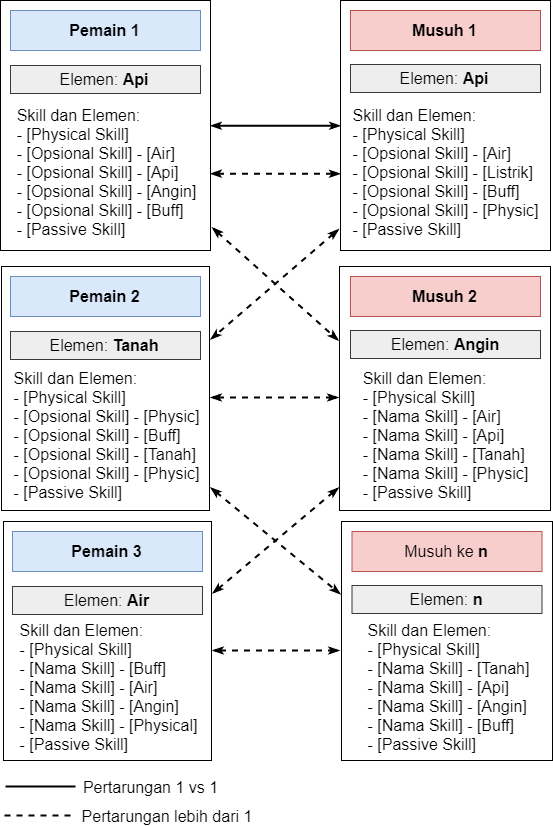
\includegraphics[scale=0.48]{img/battle_player_new.png}
	\caption{Skema pertarungan antar pemain.}
	\label{fig:battle_player}
\end{figure}

Sebelumnya pernah dijelaskan pada Sub-bab \ref{sec:sub_sec2_kesempatan} tentang meningkatnya pengambilan keputusan, pada kondisi semakin banyak musuh makan semakin banyak keputusan yang harus diambil oleh pemain. Selain itu setiap pemain memiliki elemen dan \textit{skill}, setiap elemen dapat menjadi kelemahan dan kelebihan dari setiap karakter. Hal tersebut akan membangun sebuah momen dramatis berdasarkan kompleksitas kombinasi dari musuh, hal tersebut dibahas pada Sub-bab \ref{sec:sub_sec2_kesempatan} tentang momen dramatis pada desain permainan.
\vspace{1ex}

Pada bagian ini dijelaskan contoh perancangan dari skenario pertarungan dengan jumlah karakter tunggal dan karakter pemain yang berjumlah lebih dari satu dengan dibandingkan secara langsung. Pada Gambar \ref{fig:battle_player} jika dipecah dan dijelaskan lebih lanjut maka setiap karakter yang dimainkan oleh pemain atau musuh dalam bentuk NPC (\textit{Non Playable Character}) maka bagian-bagian tersebut akan menjadi seperti beberapa poin dibawah ini.
\vspace{1ex}

\begin{enumerate}[label=\textbf{\arabic*).}]
	
	\item \textbf{Stats}
	\setlength{\parindent}{0.8cm}
	
	Atribut \textit{gameplay} yang biasa disebut dengan \textit{stats} memiliki ciri non-visual dan menyajikan informasi tentang sebuah karakter dalam permainan. Setiap permainan memiliki tipe karakteristik dapat dideskripsikan. Contohnya pada salah satu papan permainan bergenre RPG yang terkenal yaitu Dungeons and Dragons \citep{heinsoo2008}, yang memiliki enam \textit{stats} atau atribut \textit{gameplay} seperti \textit{Strength} (kemampuan fisik), \textit{Constitution} (kebugaran dan stamina), \textit{Dexterity} (Koordinasi tangan dan mata, kelincahan, reflek, dan keseimbangan), \textit{Intelligence} (Kemampuan untuk belajar dan bernalar), \textit{Wisdom} (kemampuan umum, presepsi, kedisiplinan individu), dan \textit{Charisma} (Kepribadian, kemampuan persuasif, kepemimpinan).
	\vspace{1ex}
	
	\textit{Stats} dalam RPG sangatlah diperhitungkan dan berpengaruh dalam proses pertarungan. Pada Gambar \ref{fig:rpg_turn_based} ditunjukan tidak hanya karakter pemain saja, melainkan status dari pemain saat melakukan pertarungan. Pada Gambar \ref{fig:player_stats} adalah penggambaran dari komponen atau \textit{stats} pemain yang lebih detail seperti \textit{Health Point} (HP), \textit{Attack} atau serangan, \textit{Defense} atau pertahanan, \textit{Speed} atau kecepatan.
	\vspace{1ex}
	
	\begin{figure} [!h] \centering
		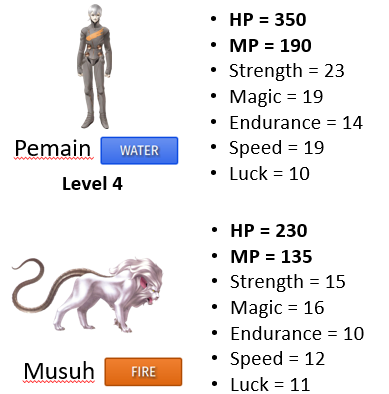
\includegraphics[scale=0.6]{img/player_stats.png}
		\caption{Status dari pemain pada permainan bergenre RPG.}
		\label{fig:player_stats}
	\end{figure}
	
	Berikut adalah penjabaran lebih dari beberapa komponen seperti HP, \textit{Attack}, \textit{Defense}, \textit{Speed} yang terdapat pada Gambar \ref{fig:rpg_turn_based}.
	
	\begin{enumerate}[label=\alph*).]
		\item \textbf{Health Point (HP)} adalah indikator nyawa atau kehidupan dari pemain, jika HP bernilai 0 maka karakter tersebut akan mati atu kalah.
		
		\item \textbf{Magic Point (MP)} adalah indikator jumlah dari jurus yang dapat dikeluarkan oleh pemain, jika MP bernilai 0 maka karakter tersebut tidak bisa mengeluarkan jurus atau kemampuan khusus.
		
		\item \textbf{Strength} adalah jumlah atau nilai serangan yang akan dilakukan untuk mengalahkan pemain lawan. Angka tersebut akan berlawanan atau dibandingkan dengan jumlah \textit{endurance} musuh. Hal tersebut bertujuan untuk mengurangi HP dari musuh.
		
		\item \textbf{Magic} atau \textit{Special Attack} biasanya tidak dimiliki oleh semua karakter pada permainan berbasis \textit{turn-based}. \textit{Special Attack} biasanya menjadi pembeda dalam setiap karakter berdasarkan jenis serangannya. Misalkan pada \textit{strength} biasanya berupa serangan fisik sedangkan pada \textit{special attack} berupa serangan \textit{magic} atau sihir.
		
		\item \textbf{Endurance} adalah jumlah atau nilai ketahanan yang digunakan oleh pemain atau musuh dalam menerima serangan. Hal ini bertujuan agar mencegah penurunan HP secara segnifikan, dengan membandingkan nilai serangan dengan nilai pertahanan.
		
		\item \textbf{Speed} atau kecepatan ada juga yang menyebutnya dengan \textit{agility} bertujuan dalam menentukan giliran dan keberhasilan dalam melakukan serangan. Semakin tinggi nilai \textit{speed}, biasanya semakin cepat melakukan serangan atau dapat mulai melakukan serangan lebih awal dibandingkan pemain atau musuh dengan nilai \textit{speed} yang lebih kecil.
		
		\item \textbf{Luck} atau keberuntungan adalah sebuah variabel yang digunakan menentukan hal yang bersifat acak, seperti bonus serangan atau \textit{critical attack}, kesempatan saat melakukan serangan balik atau \textit{counter attack} setelah diserang.
	\end{enumerate}
	
	Sementara itu skenario pertarungan dengan melibatkan \textit{stats} dijelaskan pada Gambar \ref{fig:battle_system} yang mana pemain atau musuh melakukan serangan berdasarkan \textit{speed}. Semakin tinggi \textit{speed} maka akan memperoleh giliran pertama untuk menyerang.
	\vspace{1ex}
	
	\begin{figure} [!h] 
		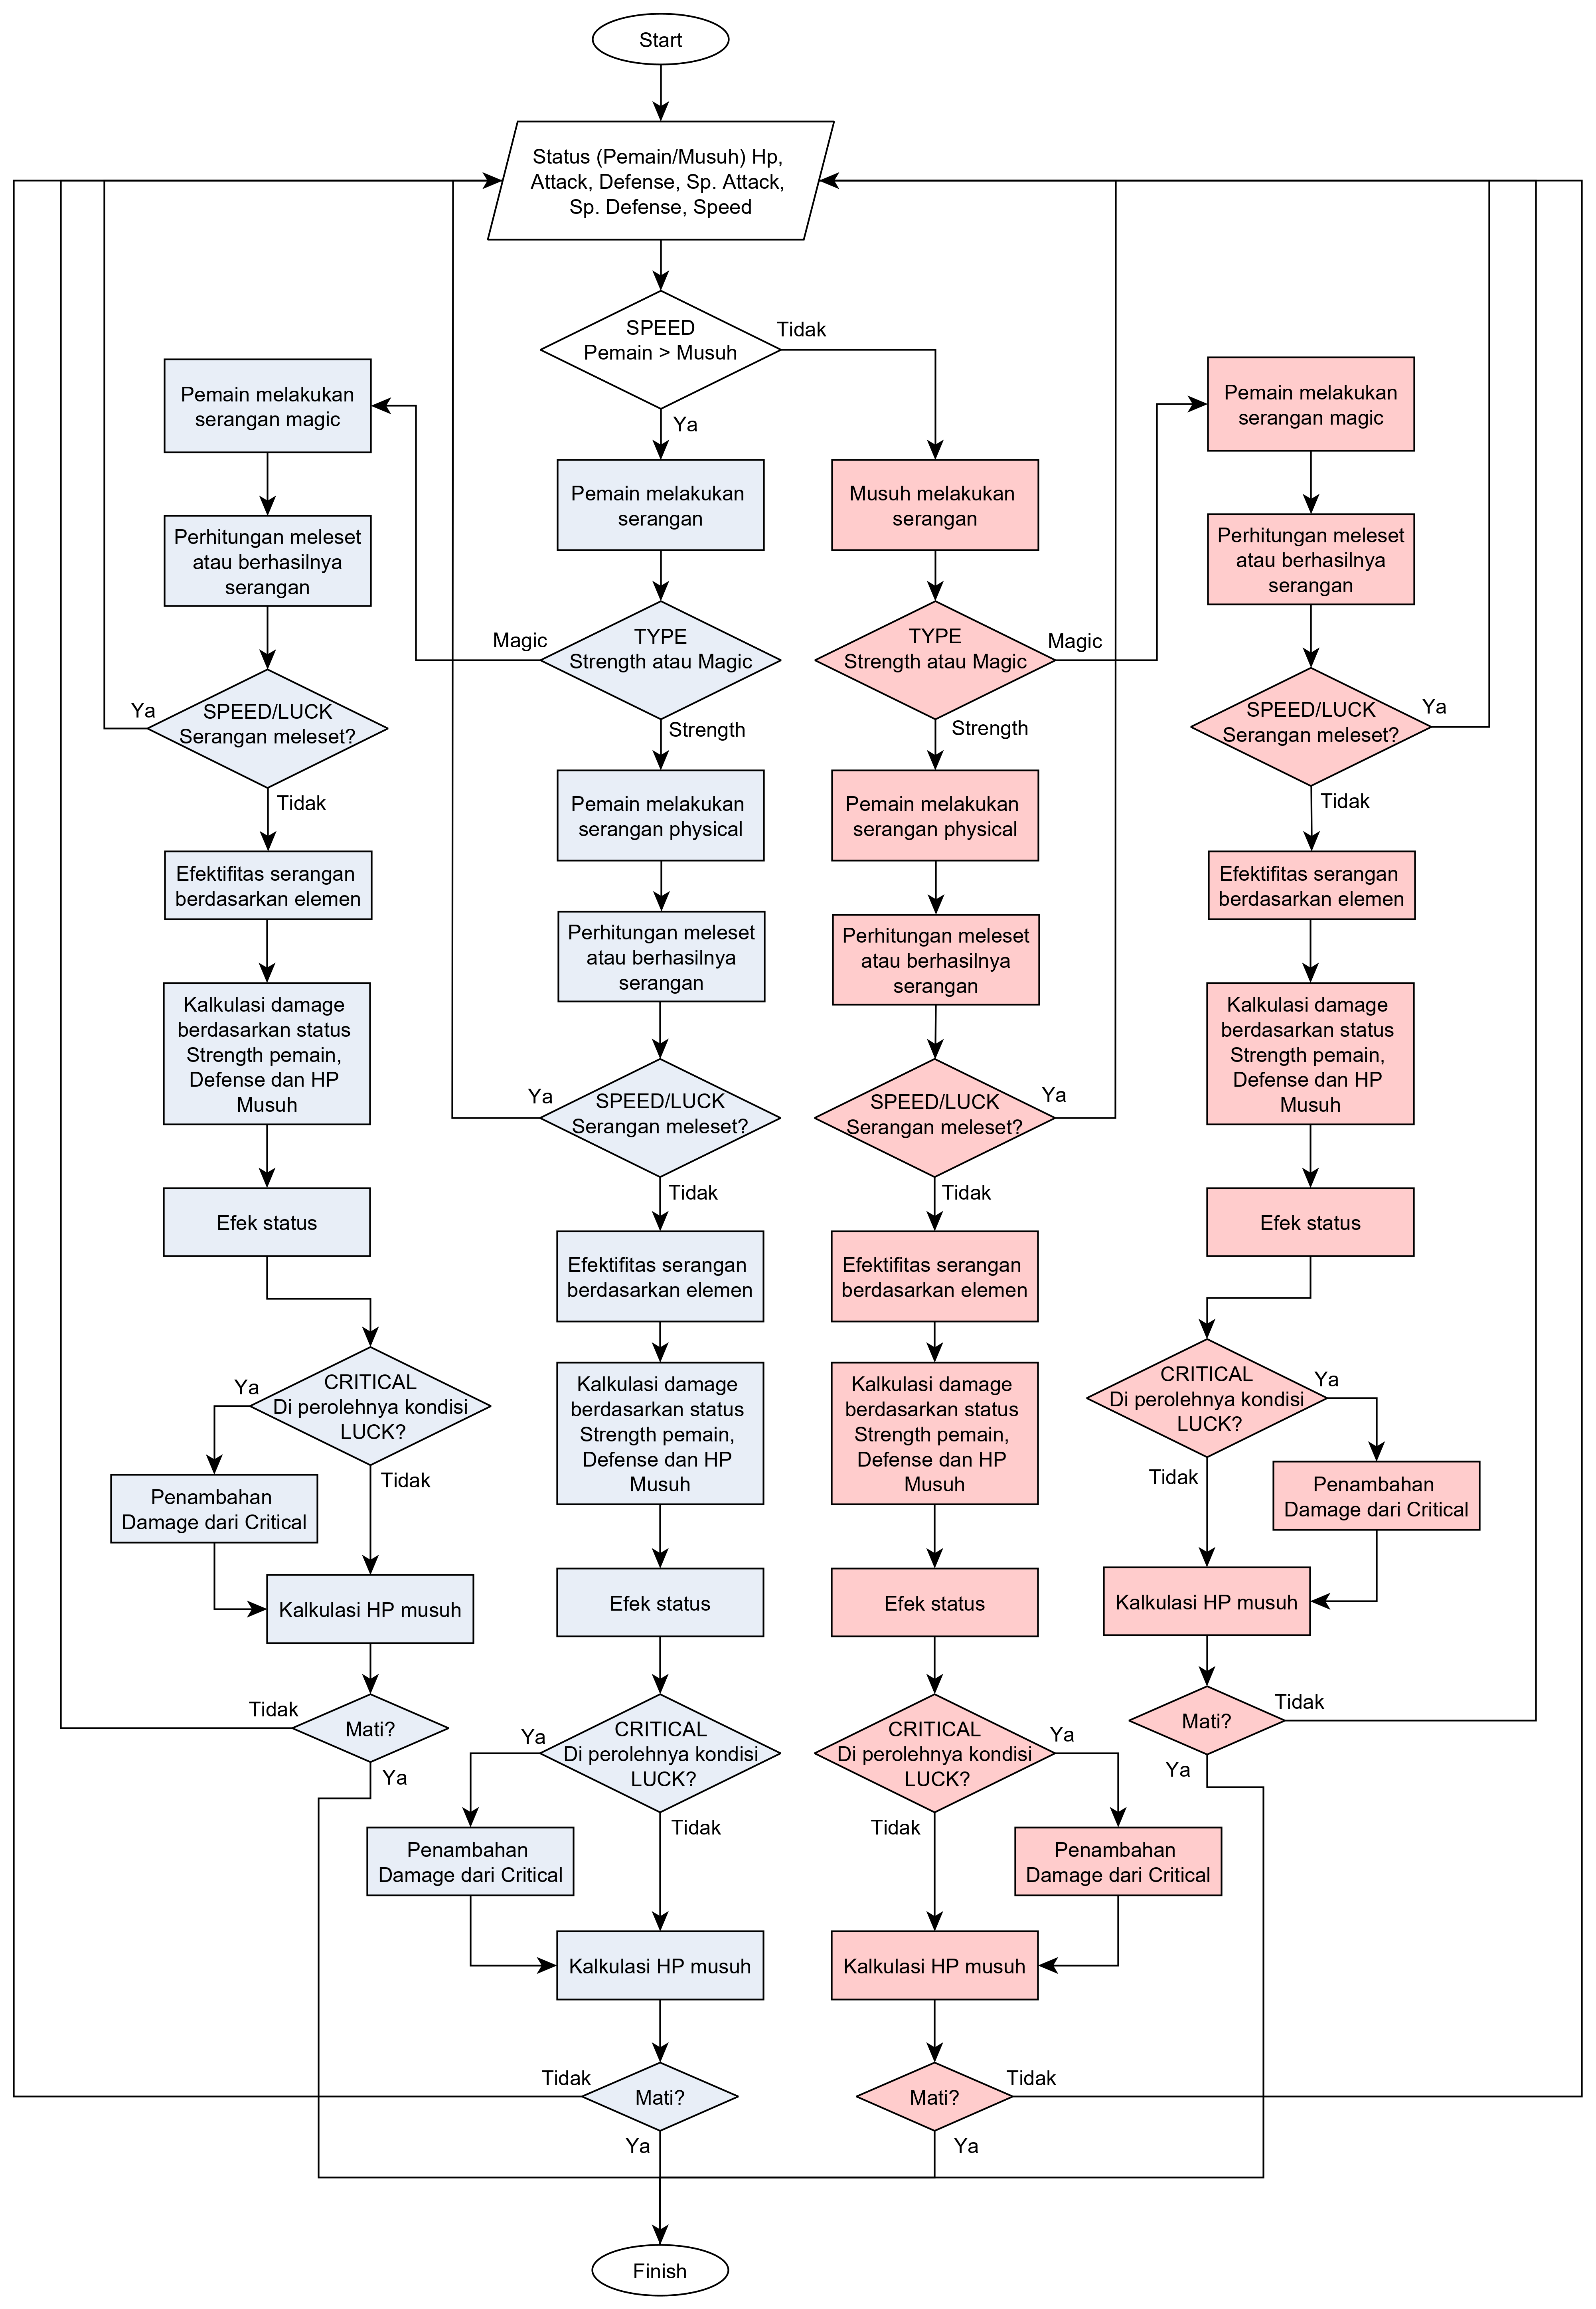
\includegraphics[scale=0.105]{img/battle_system_new_new.png}
		\caption{Skenario pertarungan \textit{turn-based}.}
		\label{fig:battle_system}
	\end{figure}
	
	Di lanjutkan lagi dengan perhitungan dengan membandingkan \textit{Speed}, dan \textit{Luck} antara karakter pemain dengan musuh, pada proses tersebutlah yang menentukan apakah serangan dari pemain dapat diterima atau meleset terhadap musuh dan sebaliknya. Tingginya \textit{Speed} pada masing-masing karakter dapat diartikan perbandingn antara kecepatan untuk menyerang dan menghindar, sedangkan \textit{Luck} adalah faktor keberuntungan yang mempengaruhi serangan tersebut. Kemudian dilanjutkan lagi dengan kalkulasi \textit{attack} dan \textit{defense} antara karakter yang menyerang dan target. Dari hasil kalkulasi tersebut akan berpengaruh pada jumlah HP dari karakter yang menjadi target.
	\vspace{1ex}
	
	Baik pada permainan RPG yang dimainkan secara \textit{real-time} atau \textit{turn-based}, keduanya melakukan mekanisme sama seperti yang dijelaskan dengan kondisi di atas. Hanya saja permainan RPG secara \textit{real-time} lebih mengandalkan ketangkasan dari pemain dalam memainkan karakter yang ingin dimainkan sepeti yang dijelaskan pada Sub-bab \ref{sec:sub_sec2_strategi} pada bagian Peran dari keterampilan pada permainan. Maka terjadilah momen saling serang secara langsung antara pemain dan musuh.
	
	\item \textbf{Elemen dan Efektifitas Serangan}
	
	Pada Gambar \ref{fig:elemen} adalah contoh elemen yang biasa digunakan dalam permainan RPG. Jumlah dari elemen dapat ditambah atau dikurangi sesuai dengan kebutuhan. Biasanya jumlah dari elemen ditentukan berdasarkan cerita. Mengapa terdapat elemen tersebut, bagaimana asal-usulnya dan sebagainya seperti yang dijelaskan pada Sub-bab \ref{sec:sub_sec3_story}.
	\vspace{1ex}
	
	\begin{figure} [!h] \centering
		
\includegraphics[scale=0.40]{img/element.png}
		\caption{Elemen pada permainan RPG.}
		\label{fig:elemen}
	\end{figure}
	
	Pembahasan ini mengacu kepada Gambar \ref{fig:battle_system} pada bagian ``efektifitas serangan berdasarkan elemen''. Sedangkan pada Gambar \ref{fig:efektifitas} adalah perbandingan pengaruh atau keterkaitan sebuah elemen dengan elemen yang lain. Di mana setiap elemen memiliki kelemahan yang berupa elemen lain dan sebaliknya. Elemen-elemen tersebut saling berlawanan satu dengan yang lainnya sehingga mampu membentuk sebuah permainan yang membutuhkan strategi khusus. Kemudian dilanjutkan dengan perhitungan \textit{stats} seperti bagian sebelumnya.
	\vspace{1ex}
	
	\begin{figure} [!h] \centering
		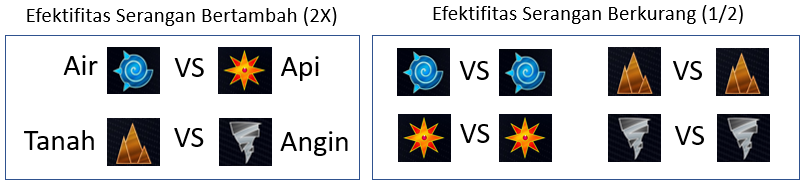
\includegraphics[scale=0.58]{img/efektifitas.png}
		\caption{Pengaruh elemen pada efektifitas serangan.}
		\label{fig:efektifitas}
	\end{figure}
	
	Jika melihat pada Gambar \ref{fig:efektifitas} dapat disimpukan bahwa beberapa element yang saling berlawanan kemudian efektifitas menjadi 2 kali lipat, contohnya pada elemen air terhadap api dan tanah terhadap angin begitu juga sebaliknya. Jika elemen yang sama saling bertarung maka efektifitasnya berkurang $1/2$ dari yang seharunya. Kemudian pada elemen lain yang belum disebutkan berlaku efektifitas normal atau 1 kali. Pembagian elemen pada pemain dan musuh akan dibahas lebih detail pada Sub-bab \ref{sec:sec3_player_stats}.
	\vspace{1ex}
	
	Kebanyakan elemen dan efektifitas serangan berlaku pada permainan RPG yang tergolong \textit{turn-based}, berbeda halnya dengan \textit{real-time} yang lebih mengandalkan keterampilan dari pemain dalam memaikan karakternya seperti yang dijelaskan pada Sub-bab \ref{sec:sub_sec2_strategi} pada bagian pemain berbasis keterampilan sepenuhnya.
	
	\item \textbf{Efek Status}
	
	Pada Gambar \ref{fig:battle_system} terdapat bagian ``efek status'', maksud dari proses tersebut adalah penambahan efek yang merugikan terhadap pemain setelah diserang. Efek kerusakan dapat membawa kesan lebih taktis pada pertempuran. Berikut adalah efek status yang akan diterapkan pada sistem pertarungan.
	
	\begin{enumerate}[label=\alph*).]
		\item \textbf{Infected:} Karakter kehilangan 10\% dari total HP setiap giliran.
		
		\item \textbf{Confused:} Karakter tidak dapat dikendalikan dan mungkin akan bertahan, menyerang dan tidak melakukan apa-apa. Ada juga kemungkinan mereka akan berbalik menyerang \textit{party member} mereka sendiri.
		
		\item \textbf{Silence:} Karakter tidak dapat mengubah Personae atau menggunakan keterampilan Persona.
		
		\item \textbf{Tired:} Karakter kehilangan SP untuk setiap tindakan yang diambil, dan menerima lebih banyak \textit{damage} dari musuh ketika diserang.
		
		\item \textbf{Hacked:} Efek yang muncul setelah target diserang sesuai dengan kelemahannya. Target kemudian akan menerima lebih banyak \textit{damage} dan tidak dapat menghindar. Jika target diserang lagi, maka statusnya akan berubah menjadi disabled.
		
		\item \textbf{Disabled:} Target akan hilang 1 giliran untuk mengambil tindakan, kemudian mendapat lebih banyak kerusakan dan serangan tidak dapat dihindari.
	\end{enumerate}
	
	Tidak semua kemampuan pemain dapat memberi efek status, hal tersebut mengacu pada desain permainan yang mengatur keseluruhan \textit{skill}, tidak hanya pada karakter utama melainkan juga pada musuh. Tetapi dalam penelitian ini, hal tersebut masih belum terpakai dikarenakan masih menyelesaikan perihal desain \textit{stats} dari pemain dan musuh. Hal ini baru semacam perkiraan saja saat mendesain sebuah permainan.
	\vspace{1ex}
	
	Pada bagian efek status juga berlaku pada permainan RPG dengan jumlah karakter tunggal, setelah berlangsungnya pertarungan antara pemain dan musuh. Di mana pada sisi pemain dapat memhangun karakternya sedemikian hingga demi memberi efek status ke pada musuh saat berlangsunnya pertarungan seperti yang dijelaskan pada Sub-bab \ref{sec:sub_sec2_strategi} tentang peran dan keterampilan pemain serta strategi dan taktik.
	
	\item \textbf{Kondisi Kritis pada Serangan}
	
	Selain \textit{attack}, elemen dan efek status, masih terdapat \textit{damage} yang dapat ditimbulkan oleh penyerang kepada target yaitu kondisi kritis pada serangan. Dengan jumlah \textit{attack} ditambah dengan jumlah \textit{attack} yang dikalikan dengan presentase tingkat kondisi kritis (\textit{critical rate}) pada \textit{skill} yang dipilih untuk menyerang lawan. Kondisi tersebut didapat dengan membandingkan nilai \textit{stats} dari \textit{Strength} atau \textit{Magic} dan \textit{luck} milik penyerang dan target, pada proses tersebutlah yang menentukan apakah serangan tersebut diperoleh kondisi kritis atau tidak. Hal tersebut juga membangun sebuah momen dramatis berdasarkan peluang terjadinya kondisi kritis saat terjadinya serangan dari pemain terlebih lagi dari musuh seperti yang dibahas pada Sub-bab \ref{sec:sub_sec2_kesempatan} tentang momen dramatis.
	
	\item \textbf{Kalkulasi HP dan MP}
	
	Pada akhirnya jumlah kerusakan yang ditimbulkan oleh penyerang dan HP dari target akan dikalkulasikan. Jika HP target habis atau sama dengan 0, maka terget tersebut dinyatakan mati. Dan jika HP target masih bersisa, maka pertarunggan akan dilanjutkan oleh giliran karakter dari pemain atau musuh selanjutnya. Kemudian pada sisi penyerang juga ada yang dikorbankan dalam upaya melakukan serangan. Saat penyerang memilih serangan fisik makan pemain akan mengorbanakan sebagian HP yang dimiliki, jika yang dipilih adalah serangan \textit{magic} maka yang dikorbankan adalah MP.
\end{enumerate}

\subsection{Hubungan Sistem Pertarungan dengan Cerita}
\label{sec:sub_sec3_story}
\vspace{1ex}

Pada setiap permainan RPG khususnya \textit{real-time} dan \textit{turn-based} RPG pasti memiliki cerita yang menjadi latar belakang permainan seperti yang dijelaskan pada Sub-bab \ref{sec:sec2_rpg}. Tentunya cerita tersebut juga memiliki pengaruh penting terhadap jumlah karakter yang dapat dimainkan oleh pemain, jumlah musuh, elemen apa saja yang akan dipakai, total waktu permainan, jumlah musuh yang harus dilawan dan lain sebagainya. Pada penelitian ini hal semacam itu akan dibuat menjadi sebuah estimasi yang kemudian disimulasikan ke dalam mode pertarungan dengan berbagai macam estimasi sebagaimana penjelasan berikut.

\begin{enumerate}[label=\textbf{\arabic*).}]
	\item \textbf{Tingkat Kesulitan Musuh}
	\setlength{\parindent}{0.8cm}

	Berikut adalah beberapa pertanyaan yang harus ditanyakan kepada setiap pembuat desain permainan:
	
	\begin{enumerate}[label=\alph*).]
		\item Haruskah kebanyakan pemain nantinya dapat menyelesaikan permainan tanpa melakukan \textit{side quest} (misi sampingan) atau melakukan \textit{grinding} (menaikan kemampuan karakter) diluar standar perkembangannya?
		\item Berapa banyak bos yang akan dilawan oleh pemain, dan seberapa jauh jaraknya? Dan bagaimana dengan penambahan bos?
		\item Berapa banyak \textit{dungeon} (tempat muncul dan bertemu dengan musuh) yang akan disajikan, dan seberapa besar \textit{dungeon} tersebut?
		\item Akankah pemain bisa menyimpan progres permainan kapan saja, atau hanya di titik penyimpanan tertentu yang sudah ditentukan?
	\end{enumerate}

	Biasanya pada permaianan RPG terdapat sebuah peta besar tentang lokasi yang merupakan latar dari cerita, tersebarlah berbagai jenis musuh yang relatif mudah dikalahkan. Kemudian ditampilkan juga beberapa \textit{dungeon} yang akan terbuka satu demi satu, yang mana \textit{dungeon} tersebut memiliki tingkat kesulitan dan kerumitan yang terus meningkat sampai dengan bertemu dengan Bos. Secara keseluruhan tingkat kesulitan juga akan terus meningkat sampai dengan akhir permaian seperti yang dicontohkan oleh Gambar \ref{fig:story_dungeon}.
	\vspace{1ex}
	
	\begin{figure} [!h] \centering
		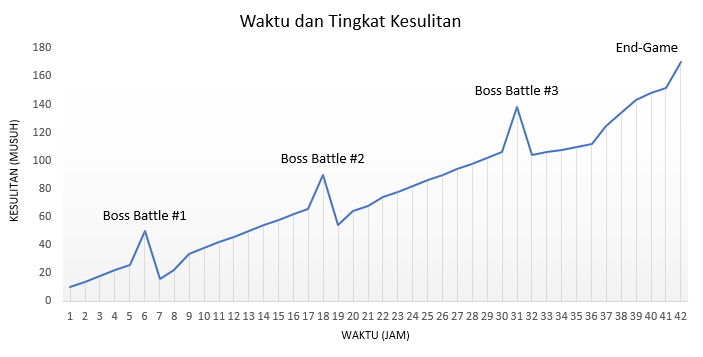
\includegraphics[scale=0.7]{img/story_dungeon.png}
		\caption{Pengaruh cerita terhadap tingkat kesulitan.}
		\label{fig:story_dungeon}
	\end{figure}
	
	Adapun beberapa cara untuk meminimalisir \textit{grinding} dan lamanya waktu permainan, dengan diberikan Exp (\textit{Experience} adalah sebuah variabel untuk pemain agar naik level) kepada pemain untuk menyelesaikan misi dan mengalahkan musuh yang lebih sulit dari pada mengalahkan musuh yang relatif mudah ditaklukan yang tersebar pada peta. Tentu saja musuh yang tersebar di peta juga memberikan Exp bagi pemain, namun seiring bertambahnya level pemain maka Exp yang diperoleh saat melawan musuh dengan level rendah akan semakin kecil.
	\vspace{1ex}
	
	Pada penelitian ini tingkat kesulitan langsung disimulasikan dengan pertarungan antara karakter-karakter yang dimainkan oleh pemain melawan musuh, dengan kondisi tingkat kesulitan musuh yang terus naik lalu turun kemudian naik lagi dan turun lagi, naik lagi dan seterusnya sampai dengan kondisi puncak. Hal ini mensimulasikan kondisi yang dilalui oleh pemain saat melawan \textit{trash mobs}, memasuki \textit{dungeon}, saat bertarung melawan bos dan kemudian pada akhirnya bertarung melawan bos terakhir. Lebih detailnya akan dijelaskan pada poin selanjutnya.

	\item \textbf{Waktu yang Diperlukan untuk Kalahkan Musuh}

	Musuh pada permainan RPG umumnya terbagi menjadi empat kategori diantaranya adalah:
	
	\begin{enumerate}[label=\Alph*).]
		\item \textit{Trash Mobs} adalah musuh yang tersebar pada seluruh area atau map.
		\item \textit{Dungeon Mobs} dapat dibagi menjadi dua sub-kategori:
		\begin{enumerate}[label=\alph*).]
			\item \textit{Dungeon Trash} atau sama seperti \textit{Trash Mobs} yang sebagian besar ditemukan awal sampai tengah \textit{dungeon}.
			\item \textit{Difficult Dungeon Trash} atau yang lebih sulit terletak lebih dekat ke bos atau dari tengah ke akhir \textit{dungeon}.
		\end{enumerate}
		\item \textit{Mini-Boss}/\textit{Boss Mobs}.
		\item \textit{End-Game Boss}/\textit{Secret Boss} (Bos yang bersifat opsional).
	\end{enumerate}
	
	Pada penelitian ini keseimbangan permainan dirancang terus meningkat seperti yang dibahas pada bagian sebelumnya, dalam permainan ini sebagian besar waktu (asumsikan saja 80\%) akan dihabiskan bertarung di dalam \textit{dungeon}. Kemudian 20\% dari waktu pertempuran akan digunakan untuk bertarung melawan bos. Sedangkan sisanya 60\% dari waktu bertarung akan dibagi antara pertarungan melawan musuh yang lemah dan juga kuat, bila digambarkan pembagian tersebut akan seperti pada Gambar \ref{fig:enemy_difficulty_percentage}.
	\vspace{1ex}
	
	\begin{figure} [!h] \centering
		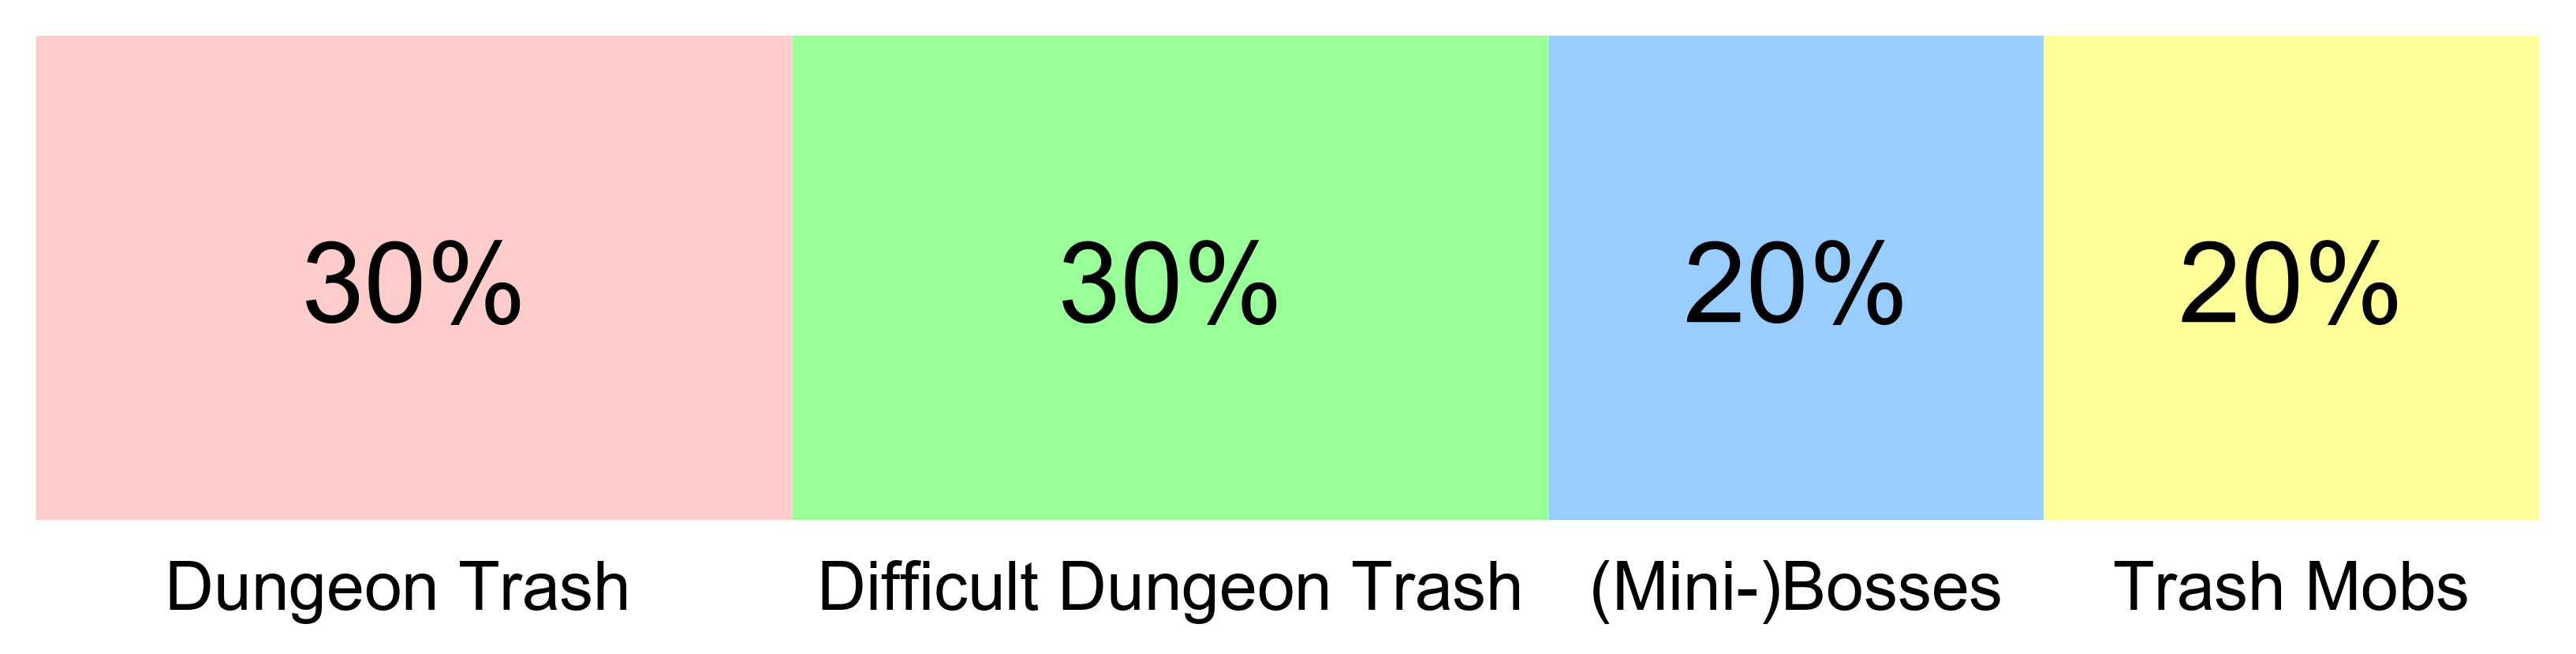
\includegraphics[scale=0.15]{img/enemy_type_distribution.png}
		\caption{Distribusi jenis musuh sesuai dengan cerita.}
		\label{fig:enemy_difficulty_percentage}
	\end{figure}
	
	Perhatikan bahwa dalam distribusi yang dibuat, jumlah waktu yang dihabiskan untuk melawan bos sama seperti waktu yang dibutuhkan untuk memerangi \textit{Thrash Mobs}. Dalam proses replikasi distribusi dalam permainan, pertama tentukan jumlah total waktu yang dibutuhkan oleh pemain untuk mengalahkan naga, raksasa atau apa pun yang biasanya disebut dengan bos.
	\vspace{1ex}
	
	Misalnya, dalam permaian RPG, bos pertama idealnya akan membutuhkan 3 menit bagi pemain yang kompeten untuk mengalahkan, dan bos terakhir menghabiskan waktu 20 menit. Kemudian terjadi peningkatan kompleksitas pada bos di level menengah, untuk terdapat dua bos yang masing-masing membutuhkan waktu sekitar 10 menit untuk dikalahkan, dan bos kedua membutuhkan waktu 7 menit.
	
	\begin{equation}
	\label{eq: total_fight}
	tB_{total} = \sum_{n = 0}^{B} tB_{n}
	\end{equation}
	
	Merujuk ke persamaan \ref{eq: total_fight} bila dijabarkan maka $tB_{total}$ adalah jumlah waktu melawan bos secara keseluruhan, jumlah bos dinyatakan dengan $B$ dan waktu yang dihabiskan untuk melawan satu bos dinyatakan dengan $tB$ kemudian diiterasi oleh $n$ sejumlah $B$.
	\vspace{1ex}
	
	Di perlukannya penyesuaian terhadap model distribusi, salah satunya waktu yang habis untuk melawan bos setara untuk melawan musuh yang mudah atau \textit{trash mobs}. Untung saja terdapat banyak cara untuk memodifikasi waktu yang akan dihabiskan saat bertarung melawan musuh yang mudah. Hal seperti menjelajah seluruh peta atau berpetualang menuju tempat-tempat sebelumnya juga tidak perlu dilakukan. Berikut adalah langkah-langkah yang dapat dilakukan:

	\begin{enumerate} [label=\alph*).]
		\item  Mengurangi atau meningkatkan tingkat pertemuan dengan musuh yang mucul secara acak atau yang biasa disebut dengan \textit{random encounter rate}. Bisa juga dengan tingkat \textit{spawn} (muncul lagi setelah mati).
		\item Menambah atau mengurangi jumlah musuh saat pertempuran.
		\item Membatasi kemampuan musuh yang menimbulkan efek status yang menyulitkan dan menghabiskan waktu seperti \textit{confused}, \textit{silence}, \textit{tired} dan lain-lain.
		\item Menambah atau mengurangi kekuatan musuh.
		\item Menambah atau mengurangi kekuatan dari \textit{party member}.
	\end{enumerate}
\end{enumerate}

Terdapat banyak fleksibilitas di sini, developer dapat mengisi daftar musuh yang akan muncul secara acak dengan musuh yang sulit dikalahkan dengan tingkat probabilitas kemunculan yang kecil, atau lebih sering memunculkan musuh yang mudah dikalahkan. Alternatif lain adalah dengan meningkatkan kekuatan \textit{party member} atau jumlah rata-rata musuh yang bertarung dalam satu kali pertarungan. Kebebasan desain semacam ini yang nantinya akan memudahkan penyeimbangan permainan. Sedangkan jumlah musuh dan panjangnya level dari pemain atau musuh sendiri menggambarkan akan lamanya permainan tersebut. Pada dasarnya semua proses diatas mengacu pada pokok pembahasan dari referensi yang dibahas pada Sub-bab \ref{sec:sub_sec2_keseimbangan} tentang menemukan keseimbangan.
\vspace{1ex}

\section{Desain Level dan Stats pada Karakter Pemain}
\label{sec:sec3_player_stats}
\vspace{1ex}

Di buatlah sebuah program yang secara otomatis dapat membuat \textit{stats} dari pemain dengan masukan sesuai dengan kebutuhan desainer permainan atau pengembang. Program tersebut terdiri dari beberapa fungsi yang pada awalnya adalah obyek yang memiliki masukan parameter-parameter yang nantinya akan menghasilkan sebuah data yang berupa \textit{stats} dari karakter pemain seperti proses yang ditunjukan oleh diagram alur pada Gambar \ref{fig:player_stats_generator}.
\vspace{1ex}

\begin{figure} [!h] \centering
	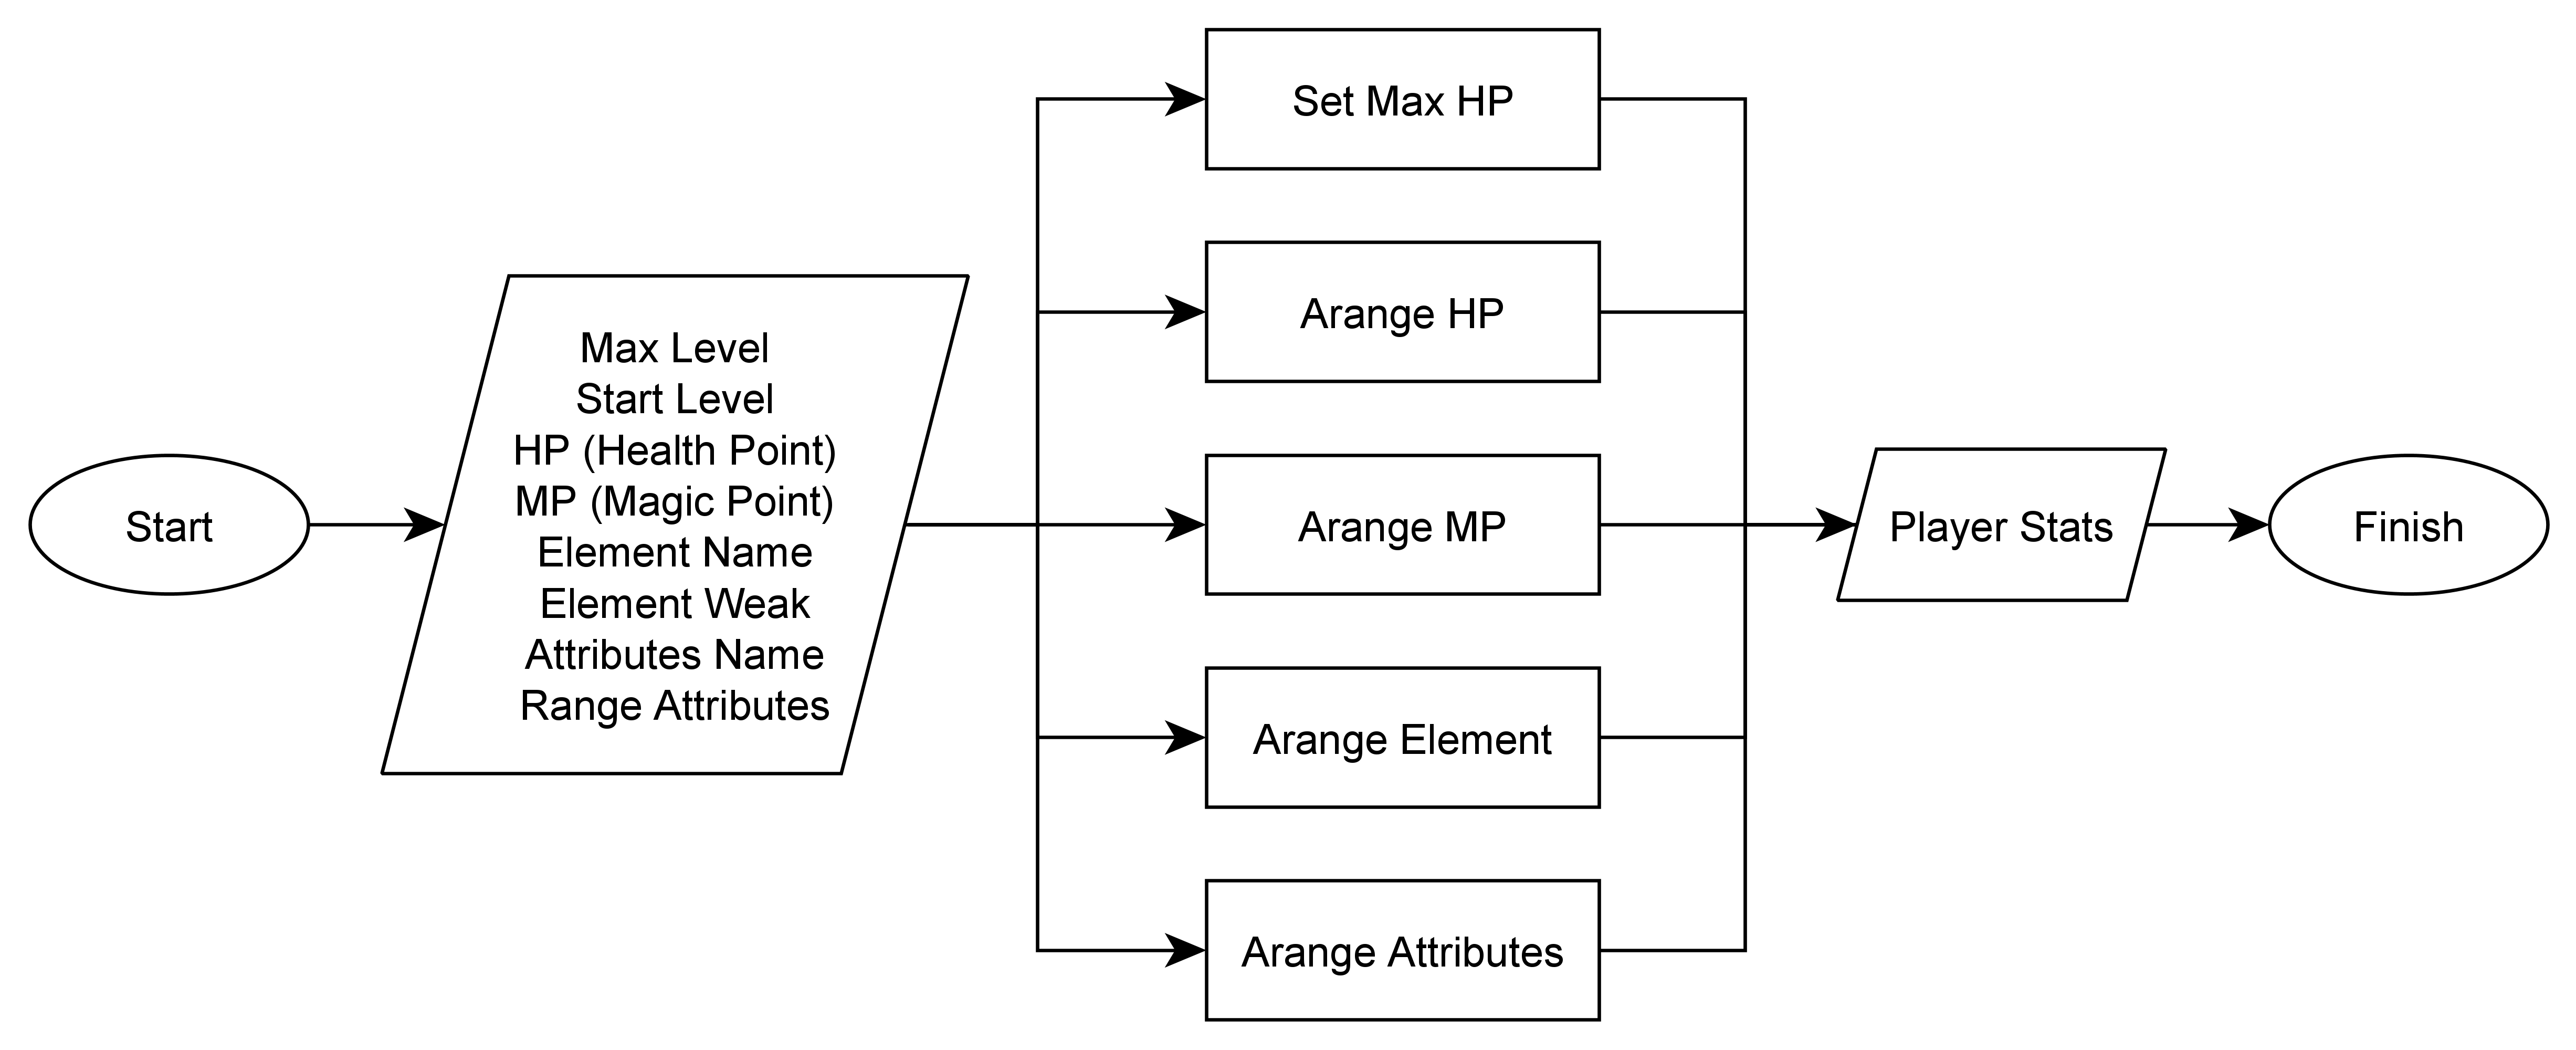
\includegraphics[scale=0.038]{img/player_stats_generator.png}
	\caption{Proses pembuatan stats untuk karakter pemain.}
	\label{fig:player_stats_generator}
\end{figure}

Pada permainan dengan genre RPG dengan jumlah karakter yang dapat dimainkan berjumlah lebih dari satu, maka program yang ditunjukan melalui proses pada Gambar \ref{fig:player_stats_generator} akan dijalankan lebih dari satu kali. Hal tersebut dilakukan dengan tujuan agar karakter utama atau yang dapat dimainkan oleh pemain berjumlah lebih dari satu. Lain halnya dengan \textit{action} RPG, cukup hanya dengan satu kali menjalankan program maka sudah diperolehnya \textit{stats} dari karakter yang dibuat. Hal tersebut dikarenakan biasanya permainan dengan genre action RPG, jumlah karakternya hanya satu.
\vspace{1ex}

Pada Gambar \ref{fig:player_stats_generator} disisi masukan program terdapat banyak sekali masukan variabel seperti \textit{Max Level} yang berupa maksimum level yang di inginkan, kemudian \textit{Start Level} yang berupa level awal dari pemain, kemudian HP yang berupa \textit{range} atau jarak antara HP terendah dengan HP terendah setelah itu. Sama halnya dengan HP, dalam perhitungan \textit{range} atau jarak pada \textit{MP} juga menggunakan cara tersebut. Kemudian \textit{Element Name} berisi daftar elemen apa saja yang ingin digunakan, begitu juga dengan \textit{Name Stats}. Kemudian untuk \textit{Range Stats} berisikan \textit{stats} awal atau inisialisasi dan maksimum \textit{stats}. Lebih detail tentang program yang dibuat dapat dilihat pada Gambar \ref{fig:player_uml}, yang merupakan \textit{class} diagram untuk membuat \textit{stats} pemain.
\vspace{1ex}

\begin{figure} [!h] \centering
	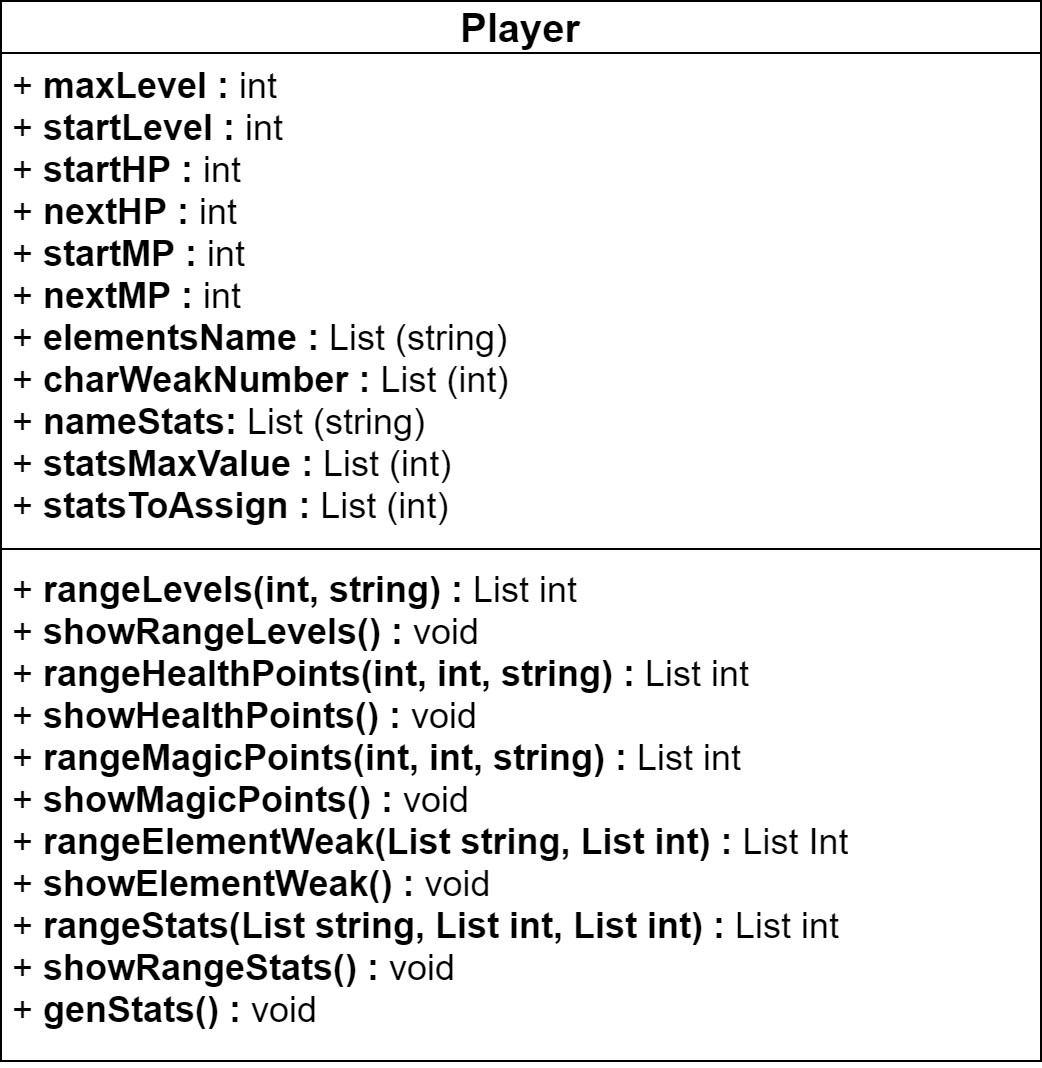
\includegraphics[scale=0.25]{img/player_uml.png}
	\caption{\textit{Class} diagram untuk \textit{stats} pemain.}
	\label{fig:player_uml}
\end{figure}

Karena program ini dibangun menggunakan OOP (\textit{Object Oriented Programming}) maka program ini dapat dijabarkan menggunakan Gambar \ref{fig:player_uml}. Selain itu program ini juga dapat secara mudah dimodifikasi untuk keperluan pengembangan kedepannya, dengan fungsi-fungsi yang ada sangat memungkinkan dilakukan \textit{override} atau pembuatan fungsi yang sama dengan isi atau proses yang berbeda.
\vspace{1ex}

Dalam menjelaskan proses pada BAB ini maka diambilah sebuah kasus dalam desain permainan, khususnya dalam penyusunan \textit{stats} untuk karakter dari pemain pada permainan RPG, baik itu permainan RPG yang tergolong \textit{real-time} atau \textit{turn-based}. Pada Tabel \ref{tb:player_input_variable} adalah masukan untuk menguji program yang akan dijelaskan pada bagian selanjutnya, yang mana masukan pada Tabel \ref{tb:player_input_variable} akan menghasilkan \textit{stats} pada sebuah karakter untuk pemain. Hal ini merupakan perwujudan dari Sub-bab \ref{sec:sub_sec3_design_skenario} bila diwujudkan dalam bentuk yang lebih teknis.
\vspace{-1ex}

\begin{longtable}{|l|l|}
	\caption{Data masukan untuk pembuatan \textit{stats} pemain.}
	\vspace{1ex}
	\label{tb:player_input_variable}\\
	\hline
	\rowcolor[HTML]{9B9B9B} 
	\multicolumn{1}{|c|}{\cellcolor[HTML]{9B9B9B}\textbf{Variabel}} & \multicolumn{1}{c|}{\cellcolor[HTML]{9B9B9B}\textbf{Input}} \\ \hline
	\textit{Start} Level & 1 \\ \hline
	\textit{Max} Level & 100 \\ \hline
	\textit{Start} HP & 159 \\ \hline
	\textit{Next} HP & 163 \\ \hline
	\textit{Start} MP & 89 \\ \hline
	\textit{Next} MP & 93 \\ \hline
	\textit{List Element} & {[} `Phys', `Water', `Wind', `Earth', `Fire' {]} \\ \hline
	\textit{List Weaknesess} & {[} 0, 0, 1, 2, 0 {]} \\ \hline
	\textit{List Stats Name} & {[} `Strength', `Magic', `Endurance', `Speed', `Luck' {]} \\ \hline
	\textit{Max Stats Value} & {[} 74, 38, 63, 65, 60 {]} \\ \hline
	\textit{Stats to Assign} & {[} 2, 1 {]} \\ \hline
\end{longtable}
\vspace{1ex}

\subsection{Distribusi Level, HP dan MP Pemain}
\label{sec:sub_sec3_player_level_hp_mp}
\vspace{1ex}

Berdasarkan Tabel \ref{tb:player_input_variable} level untuk karakter pemain dimulai dari 1 dan level maksimalnya adalah 100, pada program ini level pemain akan terus naik satu demi satu level sampai ke tingkat maksimal. Selanjutnya adalah HP atau \textit{Health Point} yang diberi masukan berupa \textit{start} HP, bisa dinyatakan juga sebagai HP saat level satu. 
\vspace{1ex}

Kemudian variabel lanjutannya adalah \textit{next} HP atau HP pada level selanjutnya, misalkan level dua. Muncul sebuah pertanyaan berapa HP selanjutnya sampai dengan level ke 100. Cara semacam itu juga berlaku untuk perhitungan MP pada program ini, dengan pola masukan yang sama dengan HP yaitu \textit{Start} MP dan \textit{Next} MP. Hal tersebut diwujudkan pada persamaan \ref{eq:hp_player} dan \ref{eq:mp_player} yang digunakan untuk mencari nilai HP dan MP selanjutnya.
\vspace{1ex}

\begin{equation}\label{eq:hp_player}
	\begin{split}
		HP = \sum_{n = 0}^{N_{p}} HP_{(n + 1)} + \left(HP_{(n + 1)} - HP_{n} \right)
	\end{split}
\end{equation}

\begin{equation}\label{eq:mp_player}
	\begin{split}
		MP = \sum_{n = 0}^{N_{p}} MP_{(n + 1)} + \left(MP_{(n + 1)} - MP_{n} \right)
	\end{split}
\end{equation}

Pada persamaan \ref{eq:hp_player} dan \ref{eq:mp_player}, HP tetap dinyatakan sebagain HP, begitu juga dengan MP. Kemudian $HP$ adalah nilai HP yang dicari, yang mana $N$ adalah level maksimum, $n$ adalah level mulai dan $n + 1$ adalah level selanjutnya. Jadi pada tahap ini seperti yang dijelaskan pada Tabel \ref{tb:player_input_variable} yang mana nilai $n$ dan $n + 1$ sudah diketahui sebagai inisialisasi, masing-masing adalah $HP_{n}$ dan $HP_{(n + 1)}$. Penjelasan ini juga berlaku untuk mencari nilai $MP$ yaitu nilai MP yang dicari. Selanjutnya melalui persamaan \ref{eq:hp_player} dan \ref{eq:mp_player} dihasilkan data dan grafik seperti yang ditunjukan pada Sub-bab \ref{sec:sub_sec4_eval_dist_hp_mp_level_single-character} dan \ref{sec:sub_sec4_eval_dist_hp_mp_level_multi-character}.
\vspace{1ex}

\subsection{Distribusi Elemen dan Kelemahan Pemain}
\label{sec:sub_sec3_list_element_player}
\vspace{1ex}

Kemudian untuk variabel \textit{List Element} berisi elemen apa saja yang akan diterapkan pada permainan tersebut, seperti yang ditunjukan oleh Tabel \ref{tb:player_input_variable}. Yang mana maksud dari variabel ini adalah memberi penjelasan dari kelemahan dan keunggulan dari pemain berdasarkan elemen, seperti yang sudah dijelasakan pada Sub-bab \ref{sec:sub_sec3_design_skenario} tentang elemen dan efektifitas serangan. Di lanjutkan dengan variabel \textit{List Weaknesses} yang memuat angka-angka yang bertujuan menggambarkan saat pemain menerima serangan dari lawan, berikut adalah penjelasan dari angka-angka tersebut.

\begin{enumerate}[label=\alph*).]
	\item \textbf{Angka 0} adalah \textit{Normal} atau efek serangan bersifat normal tanpa tambahan bonus serangan dan lain sebagainya.
	\item \textbf{Angka 1} adalah \textit{Repel} atau memiliki sifat menghindari serangan atau bahkan menghindari serangan.
	\item \textbf{Angka 2} adalah \textit{Weaknesess} atau serangan tepat menyerang terhadap kelemahan dari pemain sehingga efek kerusakan atau \textit{damage} menjadi lebih terasa, biasanya dua kali serangan normal. 
\end{enumerate}

Pembagian elemen pada pemain bersifat pada penelitian ini dibuat statis, maksudnya elemen yang dari awal didefinisikan tidak akan berubah sampai akhir level, untuk kedepannya hal seperti inilah yang akan menjadi konsetrasi pengembangan program ini berikut juga desainer permainan. Cukup dengan melakukan \textit{override} maka diperolehlah fungsi baru yang bisa menghasilkan perubahan elemen di level tertentu.
\vspace{1ex}

Pada bagian selanjutnya adalah pembahasan mengenai pembagian \textit{stats} jika merujuk pada Tabel \ref{tb:player_input_variable} dengan variabel \textit{List Stats Name} yang berisi nama atau info \textit{stats} dari pemain yang akan digunakan. Kemudian diikuti dengan variabel \textit{Max Stats Value} yang berisi nilai maksimum \textit{stats} yang akan dihasilkan. Lebih detailnya untuk bagian ini, akan dibahas secara khusus pada bagian tersendiri yaitu pada Sub-bab \ref{sec:sub_sec3_stat_pemain}.
\vspace{1ex}

\subsection{Distribusi Stats Pemain}
\label{sec:sub_sec3_stat_pemain}
\vspace{1ex}

Pada bagian ini akan dibahas tentang pembagian \textit{stats} dengan beracuan pada Tabel \ref{tb:player_input_variable} dengan variabel \textit{List Stats Name} yang berisi nama atau info \textit{stats} dari pemain yang akan digunakan. Kemudian diikuti dengan variabel \textit{Max Stats Value} yang berisi nilai maksimum \textit{stats} yang akan dihasilkan. Pada tahap ini digunakannya metode $k-$Nearest Neighbor atau $k-$NN seperti yang sudah dijelaskan pada Sub-bab \ref{sec:sub_sec2_knn} dan Naive Bayes yang juga sudah dijelaskan pada Sub-bab \ref{sec:sub_sec2_bayes}. 
\vspace{1ex}

Pada persamaan \ref{eq:KNN_distance_metrics} yang kemudian disesuaikan dengan pertambahan nilai \textit{Stats to Assign} dari Tabel \ref{tb:player_input_variable}, yang mana nilai tersebut ditambahkan secara acak antara 2 dan 1 dengan perhitungan \textit{class probability} pada persamaan \ref{eq:nbayes_class} yang disesuaikan menjadi persamaan \ref{eq:nbayes_class_stats_a} dan \ref{eq:nbayes_class_stats_b}. Hasil proses acak tersebut juga harus dibatasi jumlahnya dengan persamaan \ref{eq:KNN_distance_stats} yang akan sangat menentukan perhitungan pada persamaan \ref{eq:KNN_bayes_player_stats}.
\vspace{1ex}

\begin{equation}\label{eq:nbayes_class_stats_a}
\begin{split}
P(C_{St = 1}) = \frac{C_{St = 1}}{(C_{St = 1}\ +\ C_{St = 2})}
\end{split}
\end{equation}

\begin{equation}\label{eq:nbayes_class_stats_b}
\begin{split}
P(C_{St = 2}) = \frac{C_{St = 2}}{(C_{St = 1}\ +\ C_{St = 2})}
\end{split}
\end{equation}

\begin{equation}\label{eq:KNN_distance_stats}
\begin{split}
D(MaxSt,\ St_{n}) = \sqrt{(MaxSt - St_{n})^2}
\end{split}
\end{equation}

\begin{equation}\label{eq:KNN_bayes_player_stats}
\begin{split}
MaxSt = \left\{\begin{matrix}
\sum_{n = 0}^{N_{p}}\ St_{n}, & saat\ D(MaxSt,\ St_{n}) \geqslant 2,\ St = 2 \\ 
\sum_{n = 0}^{N_{p}}\ St_{n}, & saat\ D(MaxSt,\ St_{n}) \geqslant 1,\ St = 1 \\
\hspace{4.5em} 0, 		  & \hspace{-11.5em} lainnya
\end{matrix}\right.
\end{split}
\end{equation}

Pada persamaan \ref{eq:nbayes_class}, variabel $P(C_{St = 1})$ adalah probabilitas munculnya \textit{Stats to Assign} ke 1 dan $P(C_{St = 2})$ adalah probabilitas munculnya \textit{Stats to Assign} ke 2, kemudian $C_{St = 1}$ adalah jumlah angka satu dan $C_{St = 2}$ adalah jumlah angka dua pada \textit{Stats to Assign}. Pada dasarnya konsep munculnya \textit{Stats to Assign} adalah probabilitas yang merupakan dasar Naive Bayes seperti pada Sub-bab \ref{sec:sub_sec2_class_bayes}, kondisi tersebut menyatakan dengan probabilitas munculnya angka 0, 1, dan 2. Setiap \textit{stats} hasil pengacakan tentunya juga akan dibatasi jumlahnya dengan melakukan \textit{checking} pada maksimum \textit{stats}, hal tersebut dijelaskan pada persamaan \ref{eq:KNN_distance_stats}, yang mana $D$ adalah jarak antara $x$ maksimum \textit{stats} dan $p$ \textit{stats} saat ini. Kemudian nilai $MaxSt$ pada persamaan \ref{eq:KNN_bayes_player_stats} adalah nilai maksimum \textit{stats} yang ingin dicapai dengan jumlah $St_{n}$ sampai level maksimum atau $N_{p}$ yang dihitung oleh persamaan \ref{eq:nbayes_class_stats_a}, \ref{eq:nbayes_class_stats_b} dan \ref{eq:KNN_distance_stats}.
\vspace{1ex}

\begin{equation}\label{eq:nbayes_class_stats_1}
\begin{split}
P(C_{St = n}) = \frac{C_{St = n}}{(C_{St = 0}\ +\ C_{St = 1} +\ C_{St = n})}
\end{split}
\end{equation}

\begin{equation}\label{eq:KNN_distance_stats_1}
\begin{split}
D(MaxSt,\ St_{n}) = \sqrt{(MaxSt - St_{n})^2}
\end{split}
\end{equation}

\begin{equation}\label{eq:KNN_bayes_player_stats_1}
\begin{split}
MaxSt = \left\{\begin{matrix}
\sum_{n = 0}^{N_{p}}\ St_{n}, & saat\ D(MaxSt,\ St_{n}) \geqslant n_{st},\ St = n_{st} \\
\sum_{n = 0}^{N_{p}}\ St_{n}, & \hspace{-1.5em}saat\ D(MaxSt,\ St_{n}) \geqslant 2,\ St = 2 \\
\sum_{n = 0}^{N_{p}}\ St_{n}, & \hspace{-1.5em}saat\ D(MaxSt,\ St_{n}) \geqslant 1,\ St = 1 \\
\hspace{4.5em} 0, 		  & \hspace{-12.5em} lainnya
\end{matrix}\right.
\end{split}
\end{equation}
\vspace{1ex}

Sedangakan pada persamaan \ref{eq:nbayes_class_stats_1}, \ref{eq:KNN_distance_stats_1} dan \ref{eq:KNN_bayes_player_stats_1} digunakan saat jumlah atau dimensi \textit{Stats to Assign} lebih dari 2. Selanjutnya melalui persamaan \ref{eq:KNN_bayes_player_stats} dan beberapa persamaan yang digunakan sebelumnya pada Sub-bab \ref{sec:sub_sec3_stat_pemain} dihasilkan data seperti yang ditunjukan pada Sub-bab \ref{sec:sub_sec4_eval_single-character_stats} dan \ref{sec:sub_sec4_eval_multi-character_stats}. Pada persamaan \ref{eq:KNN_distance_stats} dan \ref{eq:KNN_distance_stats_1} adalah penggunaan perbandingan \textit{distance} atau jarak yang merupakan dasar dari $k$-NN, antara setiap kenaikan nilai \textit{stats} dan maksimum \textit{stats} yang kemudian menghasilkan grafik data berupa jumlah kenaikan \textit{stats} setiap levelnya seperti yang dijelaskan pada Sub-bab \ref{sec:sub_sec4_eval_single-character_stats}.
\vspace{1ex}

\section{Desain Level dan Stats pada Karakter Musuh}
\label{sec:sec3_enemy_stats}
\vspace{1ex}

Sama halnya dengan karakter pemain maka dibuatlah sebuah program yang secara otomatis dapat membuat \textit{stats} musuh dengan masukan sesuai dengan kebutuhan desainer permainan atau pengembang. Program tersebut terdiri dari beberapa fungsi yang pada awalnya adalah objek yang memiliki masukan parameter-parameter yang nantinya akan menghasilkan sebuah data yang berupa \textit{stats} dari karakter pemain seperti proses yang ditunjukan oleh diagram alur sederhana pada Gambar \ref{fig:enemy_stats_generator}.
\vspace{1ex}

\begin{figure} [!h] \centering
	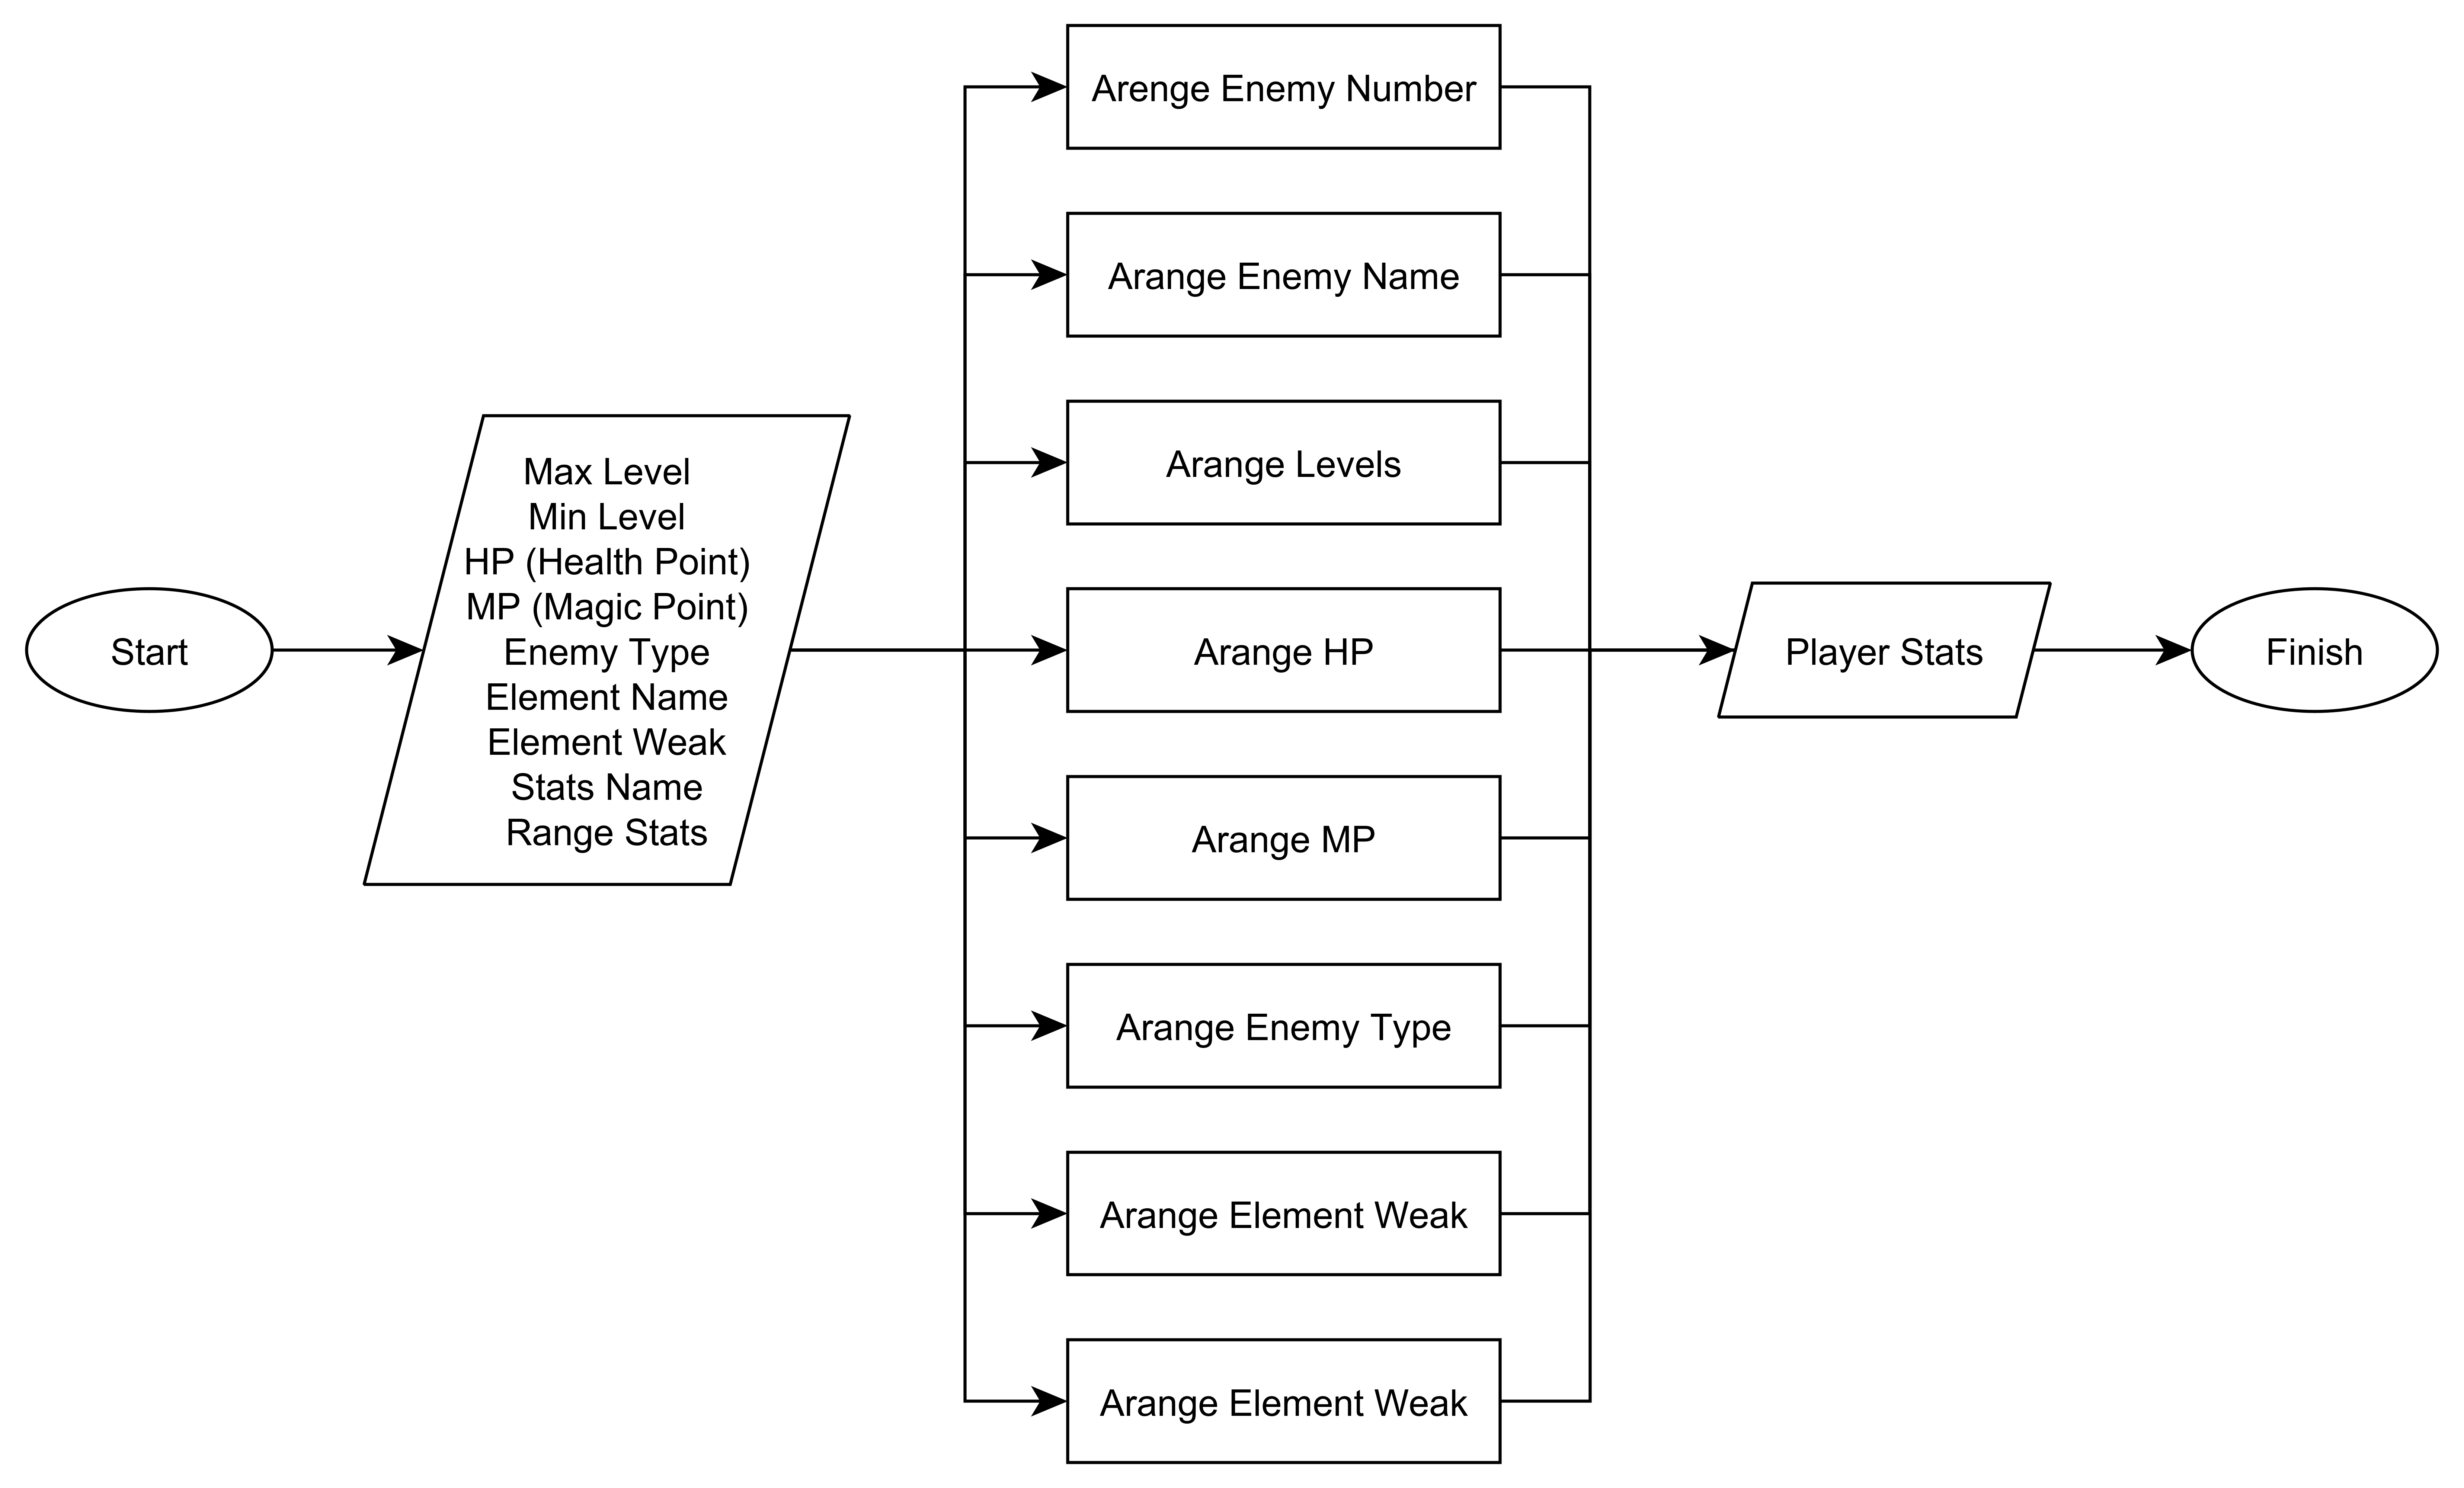
\includegraphics[scale=0.087]{img/enemy_stats_generator.png}
	\caption{Proses pembuatan \textit{stats} untuk karakter musuh.}
	\label{fig:enemy_stats_generator}
\end{figure}

Pada permainan bergenre RPG yang memiliki jumlah yang sangat banyak dan beragam, maka program yang ditunjukan melalui proses pada Gambar \ref{fig:enemy_stats_generator} dapat dijalankan satu kali saja, dan menghasilkan banyak musuh. Kecuali ingin menghasilkan kombinasi musuh yang berbeda, misalnya pada proses \textit{generate} yang pertama menghasilkan musuh yang memiliki kemampuan \textit{magic} dan kelemahan sedangkan pada kombinasi musuh selanjutnya tidak memiliki kemampuan \textit{magic}, hanya mengandalkan kemampuan fisik saja.
\vspace{1ex}

Pada Gambar \ref{fig:enemy_stats_generator} di sisi masukan program terdapat banyak sekali masukan variabel seperti \textit{Max Level} yang berupa maksimum level yang diinginkan, kemudian \textit{Min Level} yang berupa minimum level dari musuh, kemudian HP yang berupa \textit{range} atau jarak antara HP minimum dengan HP tertinggi. Sama halnya dengan HP, dalam perhitungan \textit{range} atau jarak, pada \textit{MP} juga menggunakan perhitungan dengan cara tersebut. Kemudian \textit{Enemy Type} yang berisi klasifikasi jenis \textit{stats} musuh, tergolong musuh seperti apakah \textit{stats} yang dihasilkan tersebut. 
\vspace{1ex}

Selanjutnya adalah \textit{Element Name} yang berisi daftar elemen apa saja yang dapat dipilih saat pembuatan karakter musuh, selanjutnya \textit{Element Weak} berisi tetang kelemahan dan keunggulan dari musuh tersebut ketika diserang, apakah saat diserang dengan menggunakan elemen tersebut akan mengalami kerusakan atau \textit{damage} yang parah, normal atau tidak mempan sama sekali. Kemudian untuk \textit{Stats Name} berisikan nama \textit{stats} yang dipakai dalam membuat karakter musuh. Selanjutnya adalah isi atau data dari \textit{stats} itu sendiri yang menentukan karakter dari musuh itu sendiri, seberapa kuat musuh tersebut dalam menyerang atau bertahan dan lain sebagainya. Lebih detail tentang program yang dibuat dapat dilihat pada Gambar \ref{fig:enemy_uml}, yang merupakan \textit{class} diagram untuk membuat \textit{stats} pemain.
\vspace{1ex}

\begin{figure} [!h] \centering
	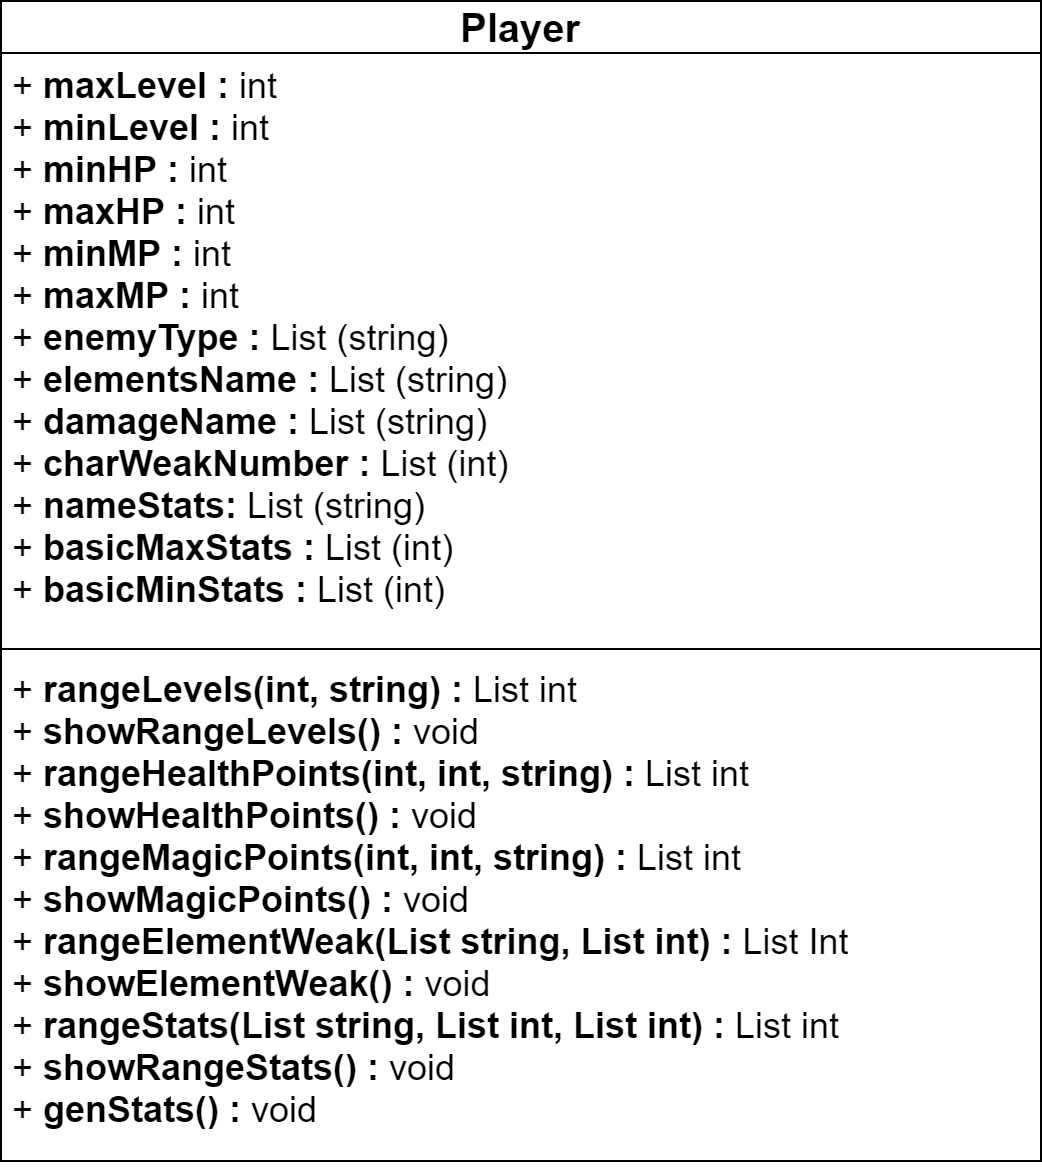
\includegraphics[scale=0.25]{img/enemy_uml.png}
	\caption{\textit{Class} diagram untuk \textit{stats} musuh.}
	\label{fig:enemy_uml}
\end{figure}

Karena program ini dibangun menggunakan OOP (\textit{Object Oriented Programming}) maka program ini dapat dijabarkan menggunakan Gambar \ref{fig:enemy_uml}. Selain itu program ini juga dapat secara mudah dimodifikasi untuk keperluan pengembangan kedepannya, dengan fungsi-fungsi yang ada sangat memungkinkan dilakukan \textit{override} atau pembuatan fungsi yang sama dengan isi atau proses yang berbeda seperti pada penjelasan dibagian pemain pada Sub-bab \ref{sec:sec3_player_stats}. Seperti pada bagian sebelumnya maka dibuatlah Tabel \ref{tb:enemy_input_variable} yang berupa masukan untuk menguji program yang akan dijelaskan pada bagian-bagian selanjutnya, yang mana masukan pada tabel tersebut akan menghasilkan \textit{stats} pada sebuah karakter untuk pemain. Sama seperti pada Sub-bab \ref{sec:sec3_player_stats} sebelumnya, yang mana pada bagian ini juga merupakan perwujudan teknis dari Sub-bab \ref{sec:sub_sec3_design_skenario} dalam bentuk yang lebih teknis.
\vspace{-1ex}

\begin{longtable}{|l|l|}
	\caption{Data masukan untuk pembuatan program pada musuh.}
	\vspace{1ex}
	\label{tb:enemy_input_variable}\\
	\hline
	\rowcolor[HTML]{9B9B9B} 
	\multicolumn{1}{|c|}{\cellcolor[HTML]{9B9B9B}\textbf{Variabel}} & \multicolumn{1}{c|}{\cellcolor[HTML]{9B9B9B}\textbf{Input}} \\ \hline
	\textit{Enemy Numbers} & 400 \\ \hline
	\textit{Max Level} & 80 \\ \hline
	\textit{Min Level} & 1 \\ \hline
	\textit{Level Class} & {[} `\textit{Easy}', `\textit{Medium}', `\textit{Hard}' {]} \\ \hline
	\textit{Min} HP & 159 \\ \hline
	\textit{Max} HP & 163 \\ \hline
	\textit{Min} MP & 89 \\ \hline
	\textit{Max} MP & 93 \\ \hline
	\textit{Enemy Type} & \begin{tabular}[c]{@{}l@{}}{[} `\textit{Mixed}', `\textit{Hard Magic}', `\textit{Soft Magic}', \\ \ \ `\textit{Hard Strength}', `\textit{Soft Magic}' {]}\end{tabular} \\ \hline
	\textit{Distribution Percentage} & {[} 40, 10, 20, 10, 20 {]} \\ \hline
	\textit{List Element} & {[} `\textit{Phys}', `\textit{Water}', `\textit{Wind}', `\textit{Earth}', `\textit{Fire}' {]} \\ \hline
	\textit{List Damage} & {[} `\textit{Normal}', `\textit{Repel}', `\textit{Weak}' {]} \\ \hline
	\textit{List Stats Name} & \begin{tabular}[c]{@{}l@{}}{[} `\textit{Strength}', `\textit{Magic}', `\textit{Endurance}',\\ \ \ `\textit{Speed}', `\textit{Luck}' {]}\end{tabular} \\ \hline
	\textit{Max Stats Value} & {[} 50, 60, 40, 55, 45 {]} \\ \hline
	\textit{Min Stats Value} & {[} 2, 2, 2, 2, 2 {]} \\ \hline
\end{longtable}

\subsection{Distribusi Level Musuh}
\label{sec:sub_sec3_enemy_level}
\vspace{1ex}

Pada bagian ini akan dijelaskan tentang pembagian level pada musuh, dengan masukan seperti yang disebutkan pada Tabel \ref{tb:enemy_input_variable}. Beracuan pada tabel tersebut beberapa variabel utama yang akan digunakan diantaranya adalah ``\textit{Enemy Numbers}'' yang menentukan jumlah musuh yang akan dibuat, ``\textit{Max Level}'' dan ``\textit{Min Level}'' adalah nilai maksimum dan minimum level musuh. Selanjutnya tingkat kesulitan dari musuh ditentukan dengan variabel ``\textit{Level Class}'' yang isinya dibagi menjadi ``\textit{Easy}'', ``\textit{Medium}'' dan ``\textit{Hard}''. Musuh dengan tingkat kesulitan \textit{``Easy''} akan menjadi yang paling mudah dikalahkan, diikuti dengan \textit{``Medium''} dan ``\textit{Hard}'' secara berurutan.
\vspace{1ex}

Kemudian terdapat variabel pendukung yang akan menentukan data atau level yang ingin dihasilkan, yaitu \textit{scale} yang disebutkan pada Tabel \ref{tb:enemy_input_variable}. Selanjutnya dilakukan beberapa proses seperti pada persamaan \ref{eq:enemy_levels1}, \ref{eq:enemy_levels2}, \ref{eq:sub_enemy_levels1}, dan persamaan \ref{eq:sub_enemy_levels2} yang kemudian diperoleh hasil berupa level untuk banyak musuh sekaligus seperti yang ditunjukan pada persamaan \ref{eq:probability_enemy_levels}.
\vspace{1ex}

\begin{equation}\label{eq:enemy_levels1}
	\resizebox{\columnwidth}{!}{%
		$SL = \left\{\begin{matrix}
		\hspace{0.2em} \sum_{i = 0}^{N_{LC}}\ \frac{LN}{N_{LC}} & Saat\ 0 \equiv LN\ (mod\ LC_{N}) & \\
		
		\hspace{0.2em} \sum_{i = 0}^{N_{LC}}\ \frac{LN}{N_{LC}} & Saat\ 0 \not\equiv LN\ (mod\ LC_{N}), & \\
		&\hspace{1.0em}  0 \not\equiv N_{LC}\ (mod\ 2) & \hspace{-3.5em} \Rightarrow\ SL_{(\left \lceil NL_{C}/2 \right \rceil)}  = \left \lceil \frac{LN}{N_{LC}} \right \rceil &\\
		
		& & \hspace{-6.0em} \Rightarrow\ SL_{i}  = \left \lfloor \frac{LN}{N_{LC}} \right \rfloor &\\
		
		\hspace{0.2em} \sum_{i = 0}^{N}\ \frac{LN}{N_{LC}} & Saat\ 0 \not\equiv LN\ (mod\ N_{LC}), & \\
		&\hspace{1.0em}  0 \equiv N_{LC}\ (mod\ 2) & \Rightarrow\ SL_{NL_{C}/2},\ SL_{(NL_{C}/2) + 1}  = \left \lceil \frac{LN}{N_{LC}} \right \rceil &\\
		
		& & \hspace{-6.0em} \Rightarrow\ SL_{i}  = \left \lfloor \frac{LN}{N_{LC}} \right \rfloor &\\
		\end{matrix}\right.$%
	}
\end{equation}

Pada persamaan \ref{eq:enemy_levels1} adalah proses pembagian \textit{range} atau banyaknya level yang dijelaskan pada Tabel \ref{tb:enemy_input_variable} pada variabel \textit{Max Level} dan \textit{Min Level} sebagai \textit{range} atau banyaknya level, disimbolkan dengan $LN$ yang kemudian dibagi dengan $N_{LC}$ yang merupakan jumlah kelompok atau \textit{cluster} dari jumlah data yang ada pada variabel \textit{Level Class}. Jika beracuan pada Tabel \ref{tb:enemy_input_variable}, maka jumlah \textit{cluster} adalah data yang ada pada varaibel ``\textit{Level Class}'' seperti ``\textit{Easy}'', ``\textit{Medium}'' dan ``\textit{High}'', jadi jumlahnya adalah 3 \textit{cluster}. Maka pada kasus yang dicontohkan ini $LC$ atau \textit{level cluster} menjadi $LC = \left \{1, 2, 3 \right \}$, saat jumlah \textit{cluster} yang ingin dibuat lebih dari contoh maka akan menjadi $LC = \left \{1, 2, 3,..., N_{LC} \right \}$ dengan $N_{LC}$ adalah jumlah \textit{cluster} yang ingin dibuat.
\vspace{1ex}

Dalam proses pencarian $SL$ atau set yang terdiri dari nilai pada setiap \textit{cluster} level atau banyaknya level dari setiap \textit{cluster} menjadi $SL = \left \{SL_{0}, SL_{1},... , SL_{i} \right\}$ yang dicontohkan terbagi menjadi tiga menjadi $SL = \left \{SL_{0}, SL_{1}, SL_{3} \right \}$, kemudian terdapat beberapa keputusan yang harus dijalankan. Seperti hasil bagi antara $LN$ dan $N_{LC}$ saat bernilai bilangan tidak bulat, maka harus dilakukan proses pembulatan dalam pembagian banyaknya level pada setiap cluster atau $SL_{i}$. Sepeti pada persamaan \ref{eq:enemy_levels1}, perlunya dilakukan pengujian, apakah hasil bagi antara $LN$ dan $N_{LC}$ berupa bilangan bulat atau tidak dengan menggunakan operasi modulus atau $mod$. Jika habis, maka setiap $SL_{i}$ akan diisi secara merata oleh hasil bagi antara $LN$ dan $N_{LC}$. Maka banyaknya level akan dibagi ke setaip \textit{cluster} adalah sebesar $LN$ dibagi dengan $LC_{N}$ yang kemudian hasil setiap \textit{cluster} disimpan dalam variabel $SL$.
\vspace{1ex}

Namun jika tidak dapat dibagi secara merata, maka dilakukan terlebih dahulu proses pengecekkan apakah jumlah $N_{LC}$ berjumlah ganjil atau genap, hal tersebut dilakukan dengan cara melakukan modulus dari $N_{LC}$ dengan angka 2. Jika ternyata $N_{LC}$ bernilai genap, maka $LN$ atau \textit{range} level akan dibagi menjadi dua bagian, kemudian dua nilai tengah setelah dibagi menjadi dua bagian tersebut diisi dengan sebaran level yang lebih banyak jika dibandingkan dengan \textit{cluster} level yang lain. Kemudian jika $LC_{N}$ bernilai ganjil maka nilai tengah dari $LN$ tersebutlah yang akan memiliki sebaran level lebih banyak jika dibandingkan dengan \textit{cluster} level yang lain.
\vspace{1ex}

Munculah pertanyaan seperti berapa banyaknya level atau $SL_{i}$ pada dua \textit{cluster} level tengah pada kasus $N_{LC}$ dengan nilai genap, dan berapakah $SL_{i}$ pada \textit{cluster} level pada bagian tengah untuk kasus $N_{LC}$ dengan nilai ganjil. Seperti pada persamaan \ref{eq:enemy_levels1} jika pada kondisi genap maka dua \textit{cluster} level bagian tengah diisi dengan level sejumlah hasil pembagian $LN$ dengan $N_{LC}$ yang dibulatkan ke atas atau \textit{ceil}, sedangkan pada kondisi ganjil maka satu \textit{cluster} level bagian tengahlah yang diisi dengan hasil pembagian tersebut. Kemudian untuk banyaknya level pada \textit{cluster} yang lain diisi dengan pembagian $LN$ dengan $LC_{N}$ yang dibulatkan ke bawah atau \textit{floor}. Jika $SL$ adalah set \textit{cluster} level, maka perlu dicari juga jumlah cluster untuk musuh dengan menggunakan persamaan \ref{eq:enemy_levels2} dengan cara sama seperti pencarian jumlah \textit{cluster} level. 
\vspace{1ex}

\begin{equation}\label{eq:enemy_levels2}
\resizebox{\columnwidth}{!}{%
	$SE = \left\{\begin{matrix}
	\hspace{0.2em} \sum_{i = 0}^{LC_{N}}\ \frac{EN}{LC_{N}} & Saat\ 0 \equiv EN\ (mod\ LC_{N}) & \\
	
	\hspace{0.2em} \sum_{i = 0}^{LC_{N}}\ \frac{EN}{LC_{N}} & Saat\ 0 \not\equiv EN\ (mod\ LC_{N}), & \\
	&\hspace{1.0em}  0 \not\equiv LC_{N}\ (mod\ 2) & \hspace{-4.0em} \Rightarrow\ SE_{(\left \lceil NL_{C}/2 \right \rceil)}  = \left \lceil \frac{EN}{LC_{N}} \right \rceil &\\
	
	& & \hspace{-6.2em} \Rightarrow\ SE_{i}  = \left \lfloor \frac{EN}{LC_{N}} \right \rfloor &\\
	
	\hspace{0.2em} \sum_{i = 0}^{LC_{N}}\ \frac{EN}{LC_{N}} & Saat\ 0 \not\equiv EN\ (mod\ LC_{N}), & \\
	&\hspace{1.0em}  0 \equiv LC_{N}\ (mod\ 2) & \Rightarrow\ SE_{NL_{C}/2},\ SE_{(NL_{C}/2) + 1}  = \left \lceil \frac{EN}{LC_{N}} \right \rceil &\\
	
	& & \hspace{-6.2em} \Rightarrow\ SE_{i}  = \left \lfloor \frac{EN}{LC_{N}} \right \rfloor &\\
	\end{matrix}\right.$%
}
\end{equation}

Dalam proses pencarian $SE$ atau \textit{cluster} musuh pada persamaan \ref{eq:enemy_levels2} digunakan cara yang sama seperti cara perhitungan pada persamaan \ref{eq:enemy_levels1} dengan membagi banyaknya musuh kedalam \textit{cluster} menjadi $SE = \left \{SE_{0}, SE_{1},... , SL_{i} \right\}$, yang dicontohkan menjadi tiga bagian $SE = \left \{SE_{0}, SE_{1}, SE_{3} \right \}$, dan dilanjutkan dengan pengambilan beberapa keputusan yang harus dijalankan. Sama seperti pada perhitungan hasil bagi antara $LN$ dan $N_{LC}$ pada persamaan \ref{eq:enemy_levels1}, nilai pembagian $EN$ atau banyaknya musuh yang dibagi dengan $LC_{N}$ atau jumlah \textit{cluster} level yang ingin dibuat dengan tiga tingkatan ``\textit{Easy}'', ``\textit{Medium}'' dan ``\textit{Hard}'' yang juga harus bernilai bilangan bulat positif, kemudian dilakukan juga proses pembulatan jumlah musuh terlebih dahulu dikarenakan jumlah musuh tidak boleh bernilai angka yang tidak bulat. 
\vspace{1ex}

Sepeti pada persamaan \ref{eq:enemy_levels1}, pada persamaan \ref{eq:enemy_levels2} juga dilakukan pengujian apakah dapat dibulatkan atau tidak maka dilakukan operasi modulus atau $mod$, jika habis maka $SE_{N}$ akan diisi secara merata oleh hasil bagi antara $EN$ dan $LC_{N}$. Maka jumlah \textit{cluster} sebanyak $N$ pada $LC_{N}$ dan banyaknya musuh adalah sebesar $EN$ yang dibagi dengan $LC_{N}$, kemudian hasil akhir tersebut disimpan dalam variabel $SE_{N}$. Untuk penjelasan langkah selanjutnya pada persamaan \ref{eq:enemy_levels2} sama persis dengan persamaan \ref{eq:enemy_levels1} yang sudah dijelaskan pada bagian sebelumnya, hanya saja objek pada persamaan \ref{eq:enemy_levels1} adalah level sedangkan pada persamaan \ref{eq:enemy_levels2} adalah musuh. Setelah $SL_{N}$ dan $SE_{N}$ diperoleh maka saatnya menuju bagian yang lebih dalam dan detail lagi. Bagaimana dengan pemberian level untuk setiap musuh, maka digunakanlah persamaan \ref{eq:sub_enemy_levels1} dan persamaan \ref{eq:sub_enemy_levels2} dengan penjelasan sebagai berikut.
\vspace{1ex}

\begin{equation}\label{eq:sub_enemy_levels1}
\resizebox{\columnwidth}{!}{%
	$SSL = \left\{\begin{matrix}
	\hspace{0.2em} \sum_{i = 0}^{N_{LC}}\ \sum_{j = 0}^{Sc}\ \frac{SL_{i}}{Sc} & Saat\ 0 \equiv SL_{i}\ (mod\ Sc) & \\
	
	\hspace{0.2em} \sum_{i = 0}^{N_{LC}}\ \sum_{j = 0}^{Sc}\ \frac{SL_{i}}{Sc} & Saat\ 0 \not\equiv SL_{i}\ (mod\ Sc), & \\
	&\hspace{1.4em}  0 \not\equiv Sc\ (mod\ 2) & \hspace{-4.5em} \Rightarrow\ SSL_{(\left \lceil Sc/2 \right \rceil)}  = \left \lceil \frac{SL_{i}}{Sc} \right \rceil &\\
	
	& & \hspace{-6.8em} \Rightarrow\ SSL_{j}  = \left \lfloor \frac{SL_{i}}{Sc} \right \rfloor &\\
	
	\hspace{0.2em} \sum_{i = 0}^{N_{LC}}\ \sum_{j = 0}^{Sc}\ \frac{SL_{i}}{Sc} & Saat\ 0 \not\equiv SL_{i}\ (mod\ Sc), & \\
	&\hspace{1.3em}  0 \equiv Sc\ (mod\ 2) & \Rightarrow\ SSL_{Sc/2},\ SSL_{(Sc/2) + 1}  = \left \lceil \frac{SL_{i}}{Sc} \right \rceil &\\
	
	& & \hspace{-6.7em} \Rightarrow\ SSL_{j}  = \left \lfloor \frac{SL_{i}}{Sc} \right \rfloor &\\
	\end{matrix}\right.$%
}
\end{equation}

Setelah diperolehnya $SL$ dan $SE$ yang masing-masing adalah set \textit{cluster} level dan set \textit{cluster} musuh, maka dicarilah $SSL$ atau set \textit{sub-cluster} level pada persamaan \ref{eq:sub_enemy_levels1} hal ini betujuan untuk mempersempit \textit{range} dalam pembagian level musuh. Seperti pada penjelasan sebelumnya terdapat satu variabel lagi yang mempengaruhi proses ini, variabel tersebut adalah $Sc$ atau skala yang digunakan untuk mentukkan kerapatan pembagian level pada musuh. 
\vspace{1ex}

Pada kasus ini $SSL$ adalah set \textit{sub-cluster} dari setiap set level \textit{cluster} atau $SL_{i}$, jadi pada dasarnya persamaan \ref{eq:sub_enemy_levels1} dijalankan setelah nilai $SL$ diperoleh dan nilai $SSL$ yang dapat berubah mengikuti nilai dari skala atau $Sc$ yang menjadi salah satu masukan pada program ini seperti yang ditulis pada persamaan \ref{eq:sub_enemy_levels1} dan \ref{eq:sub_enemy_levels2}. Perhitungan $SSL$ atau set \textit{sub-cluster} level pada dasarnya sama dengan perhitungan dalam mencari $SL$ atau $SE$ pada bagian sebelumnya, hanya saja pada bagian sebelumnya jumlah set \textit{cluster} level dan musuh dipengaruhi oleh $N_{LC}$ sedangkan pada $SSL$ jumlah set \textit{sub-cluster} level dipengaruhi oleh $Sc$.
\vspace{1ex}

Kemudian dilakukan juga pengecekan dengan operasi modulus atau $mod$ pada setiap $SL$ ke $i$ dengan $Sc$, apakah $SL_{i}$ akan habis jika dibagi dengan $Sc$. Jika ternyata $SL_{i}$ habis dibagi dengan $Sc$, maka level pada range $SSL$ atau \textit{sub-cluster} tersebut akan langsung dibagi secara merata. Sedangkan pada kondisi sebaliknya yaitu saat $SL_{i}$ tidak habis dibagi dengan $Sc$ maka akan dilakukan proses pembulatan ganjil dan genap yang dibulatkan ke atas atau \textit{ceil} seperti pada persamaan \ref{eq:enemy_levels1} dan persamaan \ref{eq:enemy_levels2}, kemudian untuk nilai yang lain dibulatkan ke bawah atau \textit{floor}.
\vspace{1ex}

\begin{equation}\label{eq:sub_enemy_levels2}
\resizebox{\columnwidth}{!}{%
	$SSE = \left\{\begin{matrix}
	\hspace{0.2em} \sum_{i = 0}^{N_{LC}}\ \sum_{j = 0}^{Sc}\ \frac{SE_{i}}{Sc} & Saat\ 0 \equiv SE_{i}\ (mod\ Sc) & \\
	
	\hspace{0.2em} \sum_{i = 0}^{N_{LC}}\ \sum_{j = 0}^{Sc}\ \frac{SE_{i}}{Sc} & Saat\ 0 \hspace{0.3em} \not\equiv SE_{i}\ (mod\ Sc), & \\
	&\hspace{1.3em}  0 \not\equiv Sc\ (mod\ 2) & \hspace{-4.5em} \Rightarrow\ SSE_{(\left \lceil SL/2 \right \rceil)}  = \left \lceil \frac{SE_{i}}{Sc} \right \rceil &\\
	
	& & \hspace{-6.6em} \Rightarrow\ SSE_{j}  = \left \lfloor \frac{SE_{i}}{Sc} \right \rfloor &\\
	
	\hspace{0.2em} \sum_{i = 0}^{N_{LC}}\ \sum_{j = 0}^{Sc}\ \frac{SE_{i}}{Sc} & Saat\ 0 \not\equiv SE_{i}\ (mod\ Sc), & \\
	&\hspace{1.2em}  0 \equiv Sc\ (mod\ 2) & \Rightarrow\ SSE_{N/2},\ SSE_{(N/2) + 1}  = \left \lceil \frac{SE_{i}}{Sc} \right \rceil &\\
	
	& & \hspace{-6.6em} \Rightarrow\ SSE_{j}  = \left \lfloor \frac{SE_{i}}{Sc} \right \rfloor &\\
	\end{matrix}\right.$%
}
\end{equation}

Kemudian untuk persamaan \ref{eq:sub_enemy_levels2} sama seperti persamaan \ref{eq:sub_enemy_levels1} hanya saja yang menjadi subjek disini adalah $SSE$ atau set \textit{sub-cluster} musuh dari setiap set level \textit{cluster} atau $SE_{i}$. Kemudian cara perhitungannya sama seperti persamaan \ref{eq:sub_enemy_levels1}, tetapi yang dibagi disini adalah setiap set \textit{cluster} atau $SE_{i}$ dari musuh dibagi dengan skala atau $Sc$. 
\vspace{1ex}

Kemudian dilakukan juga pengecekan dengan operasi modulus atau $mod$ pada setiap $SE_{i}$ dengan $Sc$, apakah $SE_{i}$ akan habis jika dibagi dengan $Sc$. Jika ternyata pada $SE$ ke $i$ habis dibagi dengan $Sc$, maka $SE$ atau banyaknya musuh dalam \textit{sub-cluster} ke $i$ akan langsung dibagi secara merata ke dalam set \textit{sub-cluster} . Sedangkan pada kondisi sebaliknya yaitu saat $SE_{i}$ tidak habis dibagi dengan $Sc$ maka akan dilakukan proses pembulatan ganjil dan genap yang dibulatkan ke atas atau \textit{ceil} seperti pada persamaan \ref{eq:enemy_levels1} dan persamaan \ref{eq:enemy_levels2}, kemudian untuk nilai yang lain dibulatkan ke bawah atau \textit{floor}.
\vspace{1ex}

Saat semua sudah selesai dilakukan, khususnya yang ada pada persamaan \ref{eq:enemy_levels1} dan persamaan \ref{eq:enemy_levels2} tentang eksekusi setiap set \textit{cluster} level dan musuh yang dilanjutkan dengan eksekusi setiap set \textit{sub-cluster} level dan musuh, pada proses tersebutlah distribusi level pada setiap musuh dilakukan. Pada persamaan \ref{eq:probability_enemy_levels} adalah penjelasan tentang peluang diperolehnya level pada setiap musuh, yang beracuan pada metode \textit{Naive Bayes} seperti yang sudah dijelaskan pada Sub-bab \ref{sec:sub_sec2_class_bayes}.
\vspace{1ex}

\begin{equation}\label{eq:probability_enemy_levels}
\begin{split}
P(Elv_{jk}) = \sum_{i = 0}^{SSL}\ \sum_{j = 0}^{SSE}\ \sum_{k = 0}^{SSE_{j}}\ \frac{Elv_{jk}}{SSL_{(i + 1)} - SSL_{i}}
\end{split}
\end{equation}

Pada persamaan \ref{eq:probability_enemy_levels} $P(Elv_{jk})$ adalah peluang munculnya level musuh yang dinyatakan dengan $Elv$, sedangkan $SSL$ adalah set dari \textit{sub-cluster} level yang merupakan alokasi persebaran level untuk musuh. Kemudian untuk $SSL$ ke $i$ dan $SSL$ ke $(i + 1)$ adalah range persebaran level untuk karakter musuh dengan alokasi setiap \textit{sub-cluster} banyaknya musuh atau $SSE_{j}$ yang kemudian setiap karakter musuh dalam \textit{sub-cluster} $SSE_{j}$ tersebut dinyatakan dengan $Elv$ ke $k$. Hasil dari proses ini kemudian dijelaskan pada Sub-bab \ref{sec:sub_sec4_eval_dist_enemy_level}.
\vspace{1ex}

Selanjutnya adalah validasi dari keseimbangan persebaran level musuh, hal ini dilakukan dengan menggunakkan beberapa langkah seperti yang ditunjukan pada persamaan \ref{eq:mean_enemy_levels}, \ref{eq:varian_enemy_levels}, \ref{eq:stdev_enemy_levels} dan persamaan \ref{eq:PDF_enemy_levels}. Konsep tersebut beracuan pada Sub-bab \ref{sec:sub_sec2_gauss_bayes} tentang \textit{Gaussian Naive bayes}, dengan harapan apakah setiap data yang dihasilkan sebelumnya sudah terdistribusi dengan normal atau tidak. Penjelasaan berikut ini adalah beberapa langkah untuk validasi keseimbangan persebaran level musuh.
\vspace{1ex}

\begin{equation}\label{eq:mean_enemy_levels}
\begin{split}
\bar{E}lv = \frac{\sum_{i = 0}^{EN}\ Elv_{i}}{EN}
\end{split}
\end{equation}

Adapun urutan metode dalam penggunaan \textit{Gaussian Naive Bayes} adalah dengan mencari rata-rata dari data tersebut, kemudian diikuti dengan perhitungan standar deviasi. Pada persamaan \ref{eq:mean_enemy_levels} adalah rata-rata dari level yang dihasilkan sama seperti pembahasan pada persamaan \ref{eq: mean} yang kemudian disimbolkan dengan variabel $\bar{E}lv$. Selanjutnya adalah $\bar{E}lv_{i}$ adalah setiap level dari musuh yang terus dijumlahkan sebanyak $LE$, yang mana $EN$ sendiri adalah banyaknya karakter musuh yang sudah dibuat. Setelah diperoleh rata-rata level maka dapat dilanjutkan dengan pencarian nilai \textit{standar deviasi} seperti pada persamaan \ref{eq:stdev_enemy_levels}.
\vspace{1ex}

\begin{equation}\label{eq:varian_enemy_levels}
\begin{split}
\sigma(Elv)^2 = \frac{\sum_{i = 0}^{EN}\ (Elv_{i} - \bar{E}lv)^{2}}{EN}
\end{split}
\end{equation}

\begin{equation}\label{eq:stdev_enemy_levels}
\begin{split}
\sigma(Elv) = \sqrt{\frac{\sum_{i = 0}^{EN}\ (Elv_{i} - \bar{E}lv)^{2}}{EN}}
\end{split}
\end{equation}

Pada persamaan \ref{eq:stdev_enemy_levels} adalah persamaan untuk mencari standar deviasi atau $\sigma(Elv)$ setelah diperolehnya rata-rata dari persebaran karakter musuh yang dinyatakan dengan $\bar{E}lv$ melalui persamaan \ref{eq:mean_enemy_levels} yang kemudian dilanjutkan dengan pencarian varian atau $\sigma(Elv)^2$ melalui persamaan \ref{eq:varian_enemy_levels} yang selanjutnya diakar kuadratkan untuk memperoleh nilai standar deviasi. Jika standar deviasi, varian dan rata-rata sudah diperoleh maka dapat dilanjutkan menuju pencarian nilai distribusi normal melalui \textit{Gausian Naive Bayes} atau Gaussian PDF (\textit{Probability Density Function}) seperti pada persamaan \ref{eq:PDF_enemy_levels} berikut ini. Hasil dari proses ini kemudian juga dijelaskan pada Sub-bab \ref{sec:sub_sec4_eval_dist_enemy_level}, yang dibuktikan dengan persebaran musuh yang terdistribusi secara normal.
\vspace{1ex}

\begin{equation}\label{eq:PDF_enemy_levels}
\begin{split}
PDF(ELv,\ \bar{E}lv,\ \sigma) = \frac{1}{\sqrt{2 \pi} \sigma}\ exp \left(-\frac{(Elv - \bar{E}lv)^2}{2 \sigma^2}\right)
\end{split}
\end{equation}

Konsep pada persamaan \ref{eq:PDF_enemy_levels} sudah sangat dijelaskan pada Sub-bab \ref{sec:sub_sec2_gauss_bayes}. Hasil perhitungaan sebelumnya yang berupa varian $\sigma^2$, rata-rata $\bar{E}lv$ dan standar deviasi $\sigma$ menjadi masukan pada persamaan tersebut. Variabel $\pi$ adalah konstanta numerik pada umumnya, kemudian fungsi $exp()$ atau $e$ adalah konstanta numerik yang betujuan untuk membentuk hasil prediksi dengan pendekatan exponensial.
\vspace{1ex}

\subsection{Distribusi Tipe Musuh}
\label{sec:sub_sec3_enemy_type}
\vspace{1ex}

Di bagian distribusi tipe musuh akan dijelaskan tentang pembagian tipe musuh, dengan masukan seperti yang disebutkan pada Tabel \ref{tb:enemy_input_variable}. Beracuan pada tabel tersebut beberapa variabel utama yang akan digunakan diantaranya adalah \textit{Enemy Type} yang menjelaskan tipe musuh yang akan dibuat. Kemudian \textit{Distribute Percentage} adalah persentase distribusi tipe yang ingin dibuat atau prentase dari \textit{Enemy Type} secara berurutan. Kemudian variabel level musuh yang diambil dan dijelaskan pada Sub-bab \ref{sec:sub_sec3_enemy_level} juga turut menentukan tipe musuh yang akan dibuat.
\vspace{1ex}

Terdapat juga variabel pendukung yang membantu proses distribusi tipe, diantaranya adalah \textit{Distribute Number} dan \textit{Distribute Level} yang keduanya perlu dicari nilainya melalui  persamaan \ref{eq:enemy_types_percentage} dan \ref{eq:enemy_types_dist_level}. Kemudian dilanjutkan denagn beberapa proses seperti pada persamaan \ref{eq:enemy_types_rest_dist_level}, dan \ref{eq:enemy_rest_types}, sehingga hal tersebut dapat direpresentasikan dengan probabilitas distribusi tipe musuh yang ditunjukan pada persamaan \ref{eq:enemy_types_probability} dan \ref{eq:enemy_types_rest_probability}.
\vspace{1ex}

\begin{equation}\label{eq:enemy_types_percentage}
\begin{split}
	\resizebox{\columnwidth}{!}{%
		$DN = \sum_{i = 0}^{N_{DP}}\ EN \times \frac{DP_{i}}{100}\ 
		\left\{\begin{matrix} 
		Saat\ \left \lceil DN_{i} \right \rceil - DN_{i} < DN_{i} - \left \lfloor DN_{i} \right \rfloor, & DN_{i} = \left \lceil DN_{i} \right \rceil \\ 
		Saat\ \left \lceil DN_{i} \right \rceil - DN_{i} > DN_{i} - \left \lfloor DN_{i} \right \rfloor, & DN_{i} = \left \lfloor DN_{i} \right \rfloor
		\end{matrix}\right.$%
	}
\end{split}
\end{equation}

Pada persamaan \ref{eq:enemy_types_percentage} adalah persamaan untuk mencari \textit{Distribute Number} atau distribusi musuh yang dinyatakan dengan $DN$ yang berupa set. Dimana nilai dari variabel tersebut menyimpan jumlah musuh disetiap tipe yang diperoleh melalui jumlah musuh $EN$, yang sebelumnya sudah dibahas pada Sub-bab \ref{sec:sub_sec3_enemy_level}. Kemudian dibandingan dengan presentase yang disiapkan sebelumnya melalui variabel masukan \textit{Distribute Percentage} atau $DP$ ke $i$, dengan $i$ adalah indeks dari set tersebut yang totalnya dinyatakan dengan $N_{DP}$, secara berurutan memuat nilai pada variabel \textit{Distribute Percentage} dalam Tabel \ref{tb:enemy_input_variable}. Keluaran dari $DN$ sendiri berupa set angaka bulat, maka dari itu setiap angka yang membentuk \textit{cluster} jumlah musuh tersebut harus dilakukan operasi pembulatan seperti pada $DN$ dengan menggunakan syarat seperti pada persamaan \ref{eq:enemy_types_percentage}. Bisa dikatakan bahwa $DN$ adalah set jumlah musuh yang ditargetkan setiap tipenya. Pendistribusian jumlah musuh pada bagian ini mengikuti jumlah angka yang ada dalam set variabel $DP$, secara berurutan angka tersebut merealisasikan persentase jumlah tipe musuh.
\vspace{1ex}

Selanjutnya adalah operasi pembagian musuh dan tipenya setelah ditemukannya $DN$, Setelah digunakan sebagai batasan dalam membagi setiap musuh berdasarkan presentase setiap tipenya. $DP$ juga digunaan sebagai pembagi tipe musuh ke setiap musuh atau musuh pada setiap level seperti pada persamaan \ref{eq:enemy_types_dist_level}, padahal $DP$ adalah sebuah variabel yang bertujuan memuat presentase pembagian jumlah musuh dan level saja. Hal ini bersifat opsional dan dapat terus dikembangkan mungkin dengan menambah variabel baru untuk mendistribusikan jumlah musuh ke dalam level dengan tidak menggunakan variabel $DP_{N}$.
\vspace{1ex}

\begin{equation}\label{eq:enemy_types_dist_level}
\begin{split}
DL = \sum_{j = 0}^{N_{DN}} \left \lfloor \frac{DN_{i}}{DP_{i}} \right \rfloor\
\left\{\begin{matrix} 
\hspace{0.5em} Saat\ i = 0, & \hspace{-4.0em}DL_{i} = DN_{i} \\ 
\hspace{1.0em} Lainnya, & DL_{i - 1} < DL_{(i - 1) + DN}
\end{matrix}\right.
\end{split}
\end{equation}

Kemudian pada persamaan \ref{eq:enemy_types_dist_level} dicarilah nilai set $DL$ yang berisi set distribusi musuh $DN_{i}$ yang masing-masing dibagi dengan set presentase tipe $DP_{i}$ seperti pada persamaan \ref{eq:enemy_types_percentage}. Hal tersebut bertujuan membentuk sebuah set yang berisi distribusi musuh dan tipenya. Bila membagi setiap musuh ke dalam presetase tipe maka tidak semua musuh dapat terbagi secara merata atau habis, seperti halnya adanya proses pembulatan dalam pendistribusian tipe pada persamaan \ref{eq:enemy_types_percentage}. Maka dicarilah sisa hasil bagi antara distribusi musuh $DN_{i}$ dengan jumlah presentase tipe $DP_{i}$ dengan persamaan \ref{eq:enemy_types_dist_level}.
\vspace{1ex}

\begin{equation}\label{eq:enemy_types_rest_dist_level}
rDL \equiv \sum_{i = 0}^{N_{DP}}\ DN_{i}\ (mod\ DP_{i})
\end{equation}

Pada persamaan \ref{eq:enemy_types_rest_dist_level} diperolehlah sisa musuh yang tidak terdistribusi yang dinyatakan dengan set $rDL$, saat dibagi setiap set jumlah musuh atau $DN_{i}$ dengan jumlah presentase tipe atau $DP_{i}$. Musuh yang belum terdistribusi nantinya akan ditambahkan atau didistribusi ke tipe sesuai hasil dari persamaan \ref{eq:enemy_types_rest_dist_level}, berupa set yang menjadi tanda bahwa terdapat musuh yang belum terdistribusi pada tipe dalam set tesebut atau $rDL_{i}$.
\vspace{1ex}

\begin{equation}\label{eq:enemy_types_probability}
P(ET_{j}) = \sum_{i = 0}^{M_{DL}} \sum_{j = 0}^{N_{EN}}\ \frac{ET_{j}}{DL_{i}}\
\left\{\begin{matrix}
\hspace{-4.6em} Saat\ ET_{j} \leq DL_{i} \\ 
Saat\ DL_{(j-1)} < ET_{j} \leq DL_{i}
\end{matrix}\right.
\end{equation}

Dari setiap musuh yang terdistribusi kedalam setiap set dari $DL$ yang dinyatakan dengan $M_{DL}$ tersebutlah kemudian dilakukan pemetaan tipe, pada kasus ini digunakanlah konsep probabilitas seperti yang dijelaskan pada persamaan \ref{sec:sub_sec2_bayes}, bila disesuaikan dengan kasus ini maka persamaan yang diperoleh akan menjadi seperti pada persamaan \ref{eq:enemy_types_probability}. Pada setiap karakter musuh $ET_{j}$ dengan $N_{EN}$ adalah jumlah musuh secara keseluruhan akan meilih satu tipe yang akan digunakannya, tipe tersebut akan menentukan \textit{stats} yang akan dijelaskan pada Sub-bab \ref{sec:sub_sec3_enemy_hp_mp_stats}. Kemudian probabilitas tipe yang dipilih $ET_{j}$ dinyatakan dengan variabel $P(ET_{i})$.
\vspace{1ex}

\begin{equation}\label{eq:enemy_rest_types}
rET = \sum_{i = 0}^{M_{EN}} EN_{i}\ -\ \sum_{i = 0}^{N_{ET}} - ET_{i}
\end{equation}

Selanjutnya pada persamaan \ref{eq:enemy_rest_types} adalah langkah untuk melihat apakah ada sisa musuh yang belum terdistribusi $rET$ dengan cara melakukan pengurangaan antara jumlah setiap musuh $EN_{i}$ yang sudah dijelaskan pada Sub-bab \ref{sec:sub_sec3_enemy_level}, yang mana $M_{EN}$ pada variabel tersebut menandakan jumlah musuh sedangan $ET_{i}$ adalah setiap musuh yang sudah memiliki tipe dengan $N_{ET}$ sebagai jumlah musuh yang sudah memiliki tipe. Pada persamaan \ref{eq:enemy_rest_types} variabel $rET$ dapat bernilai 0 saat jumlah tipe musuh $DN$ habis terbagi kedalam jumlah presentase dari tipe $DP$ seperti pada persamaaan \ref{eq:enemy_types_dist_level} dengan sisa musuh yang belum terdistribusi atau memiliki tipe yang kemudian disimpan pada variabel $rDL_{i}$ pada persamaan \ref{eq:enemy_types_rest_dist_level}. Kemudian selanjutnya adalah mendistribusikan sisa musuh yang belum memilliki tipe tersebut, seperti yang dilakukan oleh persaman \ref{eq:enemy_types_rest_probability}.
\vspace{1ex}

\begin{equation}\label{eq:enemy_types_rest_probability}
\begin{split}
\resizebox{\columnwidth}{!}{%
	$P(rET_{j}) = \sum_{i = 0}^{M_{rDL}} \sum_{j = 0}^{N_{rET}}\ \frac{ET_{j}}{rDL_{i}}\
	\left\{\begin{matrix}
	\hspace{-5.0em} Saat\ ET_{j} \leq rDL_{i}, rET > 0\\
	\hspace{0.5em} Saat\ rDL_{(i-1)} < ET_{j} \leq rDL_{i},\ rET > 0\\
	\hspace{-12.5em} Lainnya\ 0
	\end{matrix}\right.$%
}
\end{split}
\end{equation}

Dilanjutkan pada persamaan \ref{eq:enemy_types_rest_probability}, dengan dilakukannya distribusi sisa musuh yang belum memilikitipe pada $rDL$ yang berupa set penyimpan setiap sisa musuh yang dinyatakan dengan $M_{rDL}$. Kemudian setiap musuh dengan tipenya yang dinyatakan dengan $ET_{i}$, kemudian terdapat jumlah musuh belum memiliki tipe pada $rET$ yang kemudian jumlah tersebut juga dinyatakan dengan $N_{rET}$ sebagai pembatas jumlah musuh yang belum memiliki tipe, hasil dari proses tersebut kemudian digabung dengan tipe musuh yang sudah terdistribusi sebelumnya yang disimpan pada variabel $DL$. Maka variabel $P(ET_{i})$ adalah probabilitas tipe musuh yang dipilih dari distribusi level $rDL_{j}$ pada persaamaan \ref{eq:enemy_types_probability}.
\vspace{1ex}

\subsection{Distribusi Elemen dan Kelemahan Musuh}
\label{sec:sub_sec3_enemy_weak}
\vspace{1ex}

Pada persamaan \ref{eq:enemy_element} adalah penjelasan elemen yang digunakan oleh musuh seperti dideskripsikan pada Tabel \ref{tb:enemy_input_variable} pada variabel \textit{List Element}, di mana pada elemen teresebut terdapat kelemahan atau \textit{weaknesses} dan kekebalan atau \textit{repel} seperti yang dideskripsikan pada variabel \textit{List Damage} pada Tabel \ref{tb:enemy_input_variable}.  Seperti yang dijelaskan pada Sub-bab \ref{sec:sub_sec3_design_skenario} poin ke dua tentang Elemen dan Efektifitas Serangan. 
\vspace{1ex}

Pada bagian ini elemen tersebut akan dibagi ke setiap musuh dengan kondisi yang berbeda, maksudnya nanti akan ada musuh yang memiliki kelemahan dan kekebalan yang berbeda antara musuh satu dengan musuh yang lain. Misalkan \textit{Enemy 1} memiliki kelemahan api atau \textit{fire} yang mana HP akan berkurang dua kali jika diserang dengan menggunakan elemen api dan memiliki kekebalan air atau \textit{water} yang mana karakter tersebut kebal saat diserang dengan \textit{skill} dari elemen air. Kemudian pada \textit{Enemy 2} berbeda dengan \textit{Enemy 1}, misalnya pada \textit{Enemy 1} memiliki kelemahan api sedangkan pada \textit{Enemy 2} memiliki kelemahan air misal dan kebal terhadap angin atau \textit{wind}. Kemudian daftar elemen yang akan digunakan mengacu pada Tabel \ref{tb:enemy_input_variable} pada variabel \textit{List Element} yang berisi \textit{Phys} atau fisik, \textit{Water} atau air, \textit{Wind} atau angin, \textit{Earth} atau tanah dan \textit{Fire} atau api. Kemudian urutan efek serangan juga dinyatakan pada Tabel \ref{tb:enemy_input_variable} dengan variabel List Damage yang berisi \textit{Normal}, \textit{Repel} dan \textit{Weak}. Dimana penjelasan untuk setiap elemen dan efek serangan sudah dijelaskan sebelumnya pada Sub-bab \ref{sec:sub_sec3_design_skenario}.
\vspace{1ex}

\begin{equation}\label{eq:enemy_element}
\resizebox{0.2\textwidth}{!}{%
	$ElN = \left\{\begin{matrix}
	\hspace{-0.34em} Phys \\ 
	\hspace{0.3em} Water \\
	\hspace{0.0em} Wind \\
	\hspace{0.2em} Earth \\
	\hspace{-0.3em} Fire \\
	\hspace{-1.6em} ... \\
	\hspace{-1.6em} n
	\end{matrix}\right.$%
}
\end{equation}

Pada dasarnya satu karakter musuh tidak akan menggunakan seluruh elemen yang ada pada persamaan \ref{eq:enemy_element} yang merupakan penggambaran dari varaibel \textit{List Element} pada Tabel \ref{tb:enemy_input_variable}, mungkin hanya sekitar satu sampai dengan tiga. Maka dari itu kondisi tersebut dapat dinyatakan dengan kondisi $DmgNa \in ElN$, yang mana seluruh elemen bisa menjadi kelemahan atau kekebalan dari musuh. Sama seperti pada persamaan \ref{eq:enemy_element} yang mana $ElN$ adalah nama elemen, sedangkan $DmgNa$ adalah \textit{damage name} atau nama dari efek serangan yang dilakukan. Di mana pada persamaan \ref{eq:damage_name_number} $DmgNa$ akan dipilih secara acak dengan persamaan \ref{eq:damage_number_prob}, yang akan menjadi kelemahan atau kekebalan terhadap serangan dari pemain seperti pada persamaan \ref{eq:damage_name_number}. Pada persamaan \ref{eq:damage_name_number} sendiri adalah penggambaran dari variabel \textit{List Damage} pada Tabel \ref{tb:enemy_input_variable}. 
\vspace{1ex}

\begin{equation}\label{eq:damage_name_number}
\resizebox{0.5\textwidth}{!}{%
	$DmgNu = \left\{\begin{matrix} 
	\hspace{0.0em} 0,  & \hspace{-7.0em} Normal \\
	\hspace{0.0em} 1,  & \hspace{-8.0em} Repel \\
	\hspace{0.0em} 2,  & \hspace{-7.7em} Weak \\
	\hspace{0.5em} ... & \\
	\hspace{0.5em} n,  & Defined\ Status\ Name
	\end{matrix}\right.$%
}
\end{equation}

Kemudian pada persamaan \ref{eq:damage_name_number}, variabel $DmgNu$ adalah respon atau efek dari serangan yang yang dikonversi menjadi angka, yang pada mulanya berupa nama respon atau efek setelah diserang. Kemudian hasil pemilihan tersebut disimpan pada variabel $DmgNu$ yang dapat dinyatakan dengan persamaan \ref{eq:damage_number_prob}.
\vspace{1ex}

\begin{equation}\label{eq:damage_number_prob}
P(DmgNu) = \frac{DmgNu}{\sum_{i = 0}^{N_{Na}}\ DmgNa_{i}}
\end{equation}

Pada persamaan \ref{eq:damage_name_number} terdapat set variabel $DmgNa$ yang dipilih secara acak sebagai elemen yang nantinya akan memiliki respon khusus terhadap serangan yang dinyatakan dengan $DmgNu$, selanjutnya angka yang deperoleh berupa indeks yang dipilih dari jumlah element atau $N_{Na}$ seperti yang dinyatakan dalam persamaan \ref{eq:damage_number_prob}. Jadi dari $DmgNa$ akan dipilih satu sampai dengan tiga elemen secara acak yang kemudian menjadi kelemahan atau kekebalan dari karakter musuh tersebut. Namun pada persamaan \ref{eq:damage_number_prob}, hanya merepresentasikan satu efek serangan saja. Maka dilanjutkan dengan persamaan \ref{eq:multi_damage_num_prob}, agar dalam satu karter musuh bisa memiliki lebih dari satu efek serangan.

\begin{equation}\label{eq:multi_damage_num_prob}
P(DmgNu_{i}) = \sum_{i = 0}^{M_{Nu}}\ \frac{DmgNu_{i}}{\sum_{j = 0}^{N_{Na}}\ DmgNa_{j}}
\end{equation}

Sedangkan pada persamaan \ref{eq:multi_damage_num_prob} adalah penjelasan tentang proses munculnya setiap $DmgNu$ pada satu karakter musuh, sehingga variabel tersebut berubah menjadi $DmgNu_{i}$ dengan $M_{Nu}$ adalah jumlah dari respon atau efek saat musuh menerima serangan. Seperti penjelasan sebelumnya bahwa pada sebuah karakter musuh dapat memiliki lebih dari satu kelemahan atau kekebalan $DmgNu$ dari $DmgNa$ yang dipilih secara acak seperti yang sudah dijelaskan pada bagian sebelumnya. Berkaca pada persamaan \ref{eq:damage_number_prob} dan \ref{eq:multi_damage_num_prob}, penggunaan Naive bayes dengan dasar probabilitas diterapkan pada kedua persamaan tersebut yang mengacu dengan penjelasa pada Sub-bab \ref{sec:sub_sec2_class_bayes}.
\vspace{1ex}

\begin{equation}\label{eq:all_enemies_damage}
DmgEN = \sum_{i = 0}^{EN}\sum_{j = 0}^{N_{Nu}} DmgNu_{ij}
\end{equation}

Selanjutnya adalah proses penerapan persamaan \ref{eq:multi_damage_num_prob} ke seluruh karakter musuh yang dinyatakan dengan variabel set $DmgEN$ seperti pada persamaan \ref{eq:all_enemies_damage}, $DmgEN$ berupa set variabel yang berisi persebaran $DmgNu$ dan elemennya $DmgNa$ pada setiap karakter musuh. Sesuai dengan persamaan \ref{eq:all_enemies_damage}, yang mana $EN$ adalah jumlah musuh sedangkan $N_{Nu}$ adalah jumlah $DmgNu$ pada satu musuh yang berjumlah satu sampai dengan tiga seperti yang sudah dijelaskan pada paragraf sebelumnya pada Sub-bab ini.
\vspace{1ex}

\subsection{Distribusi HP, MP, dan Stats Musuh}
\label{sec:sub_sec3_enemy_hp_mp_stats}
\vspace{1ex}

Bila melihat pada Tabel \ref{tb:enemy_input_variable} terdapat beberapa variabel seperti \textit{List Stats Name}, \textit{Max Stats Value}, dan \textit{Min Stats Value}. Variabel tersebut akan nantinya akan digunakan untuk membuat \textit{stats} untuk karakter musuh dengan basis algorima Naive Bayes. Di awali dengan persamaan \ref{eq:enemy_types_stats_ex} yang menjadi pembagi setiap operasi pembagian \textit{stats} berdasarkan tipe.
\vspace{1ex}

\begin{equation}\label{eq:enemy_types_stats_ex}
\resizebox{0.4\textwidth}{!}{%	
	$ET = \sum_{i= 0}^{N} ET_{i} \left\{\begin{matrix}
	ET_{i} = 0, & MX\\ 
	ET_{i} = 1, & HM\\ 
	ET_{i} = 2, & SM\\ 
	ET_{i} = 3, & HS\\
	ET_{i} = 4, & SS
	\end{matrix}\right.$%
}
\end{equation}

Pada persamaan \ref{eq:enemy_types_stats_ex} yang merepresentasikan masukan variabel pada Tabel \ref{tb:enemy_input_variable}, sedangkan pada persaamaan \ref{eq:enemy_types_stats_adv} adalah pengembangan jika jumlah tipe musuh dinaikkan lebih dari yang dicontohkan pada Tabel \ref{tb:enemy_input_variable} pada variabel \textit{Enemy Type}. Pada kedua persamaan tersebut terdaapat beberapa variabel diantaranya adalah $ET_{i}$ yang yang menyatakan tipe musuh ke $i$, kemudian secara berurutan masing-masing $MX$, $HM$, $SM$, $HS$, dan $SS$ adalah musuh dengan tipe \textit{mixed}, \textit{hard magic}, \textit{soft magic}, \textit{hard strength}, dan \textit{soft strength}.
\vspace{1ex}

\begin{equation}\label{eq:enemy_types_stats_adv}
\resizebox{0.4\textwidth}{!}{%
	$ET_{i} = \sum_{i= 0}^{N} ET_{i} \left\{\begin{matrix}
	ET_{i} = 0, & MX\\ 
	ET_{i} = 1, & HM\\ 
	ET_{i} = 2, & SM\\ 
	ET_{i} = 3, & HS\\ 
	ET_{i} = 4, & SS\\
	... & ... \\
	\hspace{0.2em} ET_{N} = N, & ST_{N}
	\end{matrix}\right.$%
}
\end{equation}

Kemudian pada persamaan \ref{eq:enemy_types_stats_adv} secara spesifik terdapat variabel $ET_{N}$ yang merupakan variabel tipe musuh ke $N$ atau batas jumlah musuh. Variabel $i$ adalah urutan dari indeks setiap tipe musuh yang dideskripsikan, berikut juga variabel $ST_{N}$, dengan variabel $ST$ adalah \textit{stats} dan $N$ adalah batas jumlah musuh. Selanjutnya adalah dilakukannya pembagian tipe musuh jika musuh tersebut memiliki tipe $MX$ atau \textit{mixed} seperti pada persamaan \ref{eq:enemy_types_stats_mixed_ex}.
\vspace{1ex}

\begin{equation}\label{eq:enemy_types_stats_mixed_ex}
MX = \sum_{i= 0}^{N_{MX}} MX_{i} \left\{\begin{matrix}
MX_{i} = 1, & MP\ Focused\\
MX_{i} = 2, & HP\ Focused
\end{matrix}\right.
\end{equation}

Pada persamaan \ref{eq:enemy_types_stats_mixed_ex} terdapat variabel $MX_{i}$ yang merupakan variabel satuan dari musuh yang bertipe \textit{mixed} yang dinyatakan dengan $N_{MX}$. Kemudian pada variabel $MX$ yang berupa set atau memuat banyak variabel musuh yang bertipe \textit{mixed}. Pada persamaan \ref{eq:enemy_types_stats_mixed_ex} sendiri dijelaskan bahwa pada tipe \textit{mixed} dipecah menjadi dua tipe lagi, yang satu berfokus pada $HP$ dan satu lagi pada $MP$. Jadi isi dari variabel $MX$ nantinya akan terdiri dari musuh bertipe \textit{mixed} dengan bagian tipe MP atau berfokus pada MP dan sub-tipe HP atau berfokus pada HP.
\vspace{1ex}

\begin{equation}\label{eq:enemy_types_stats_mixed_adv}
Mx = \sum_{i= 0}^{N_{MX}} Mx_{i} \left\{\begin{matrix}
\hspace{0.6em} Mx_{i} = 1, & MP\ Focused\\
\hspace{0.6em} Mx_{i} = 2, & HP\ Focused\\
\hspace{0.6em} ... & \hspace{-2.0em} ... \\
\hspace{0.8em} Mx_{N} = n, & \hspace{-2.0em} Lainnya\\
\end{matrix}\right.
\end{equation}

Pada persamaan \ref{eq:enemy_types_stats_mixed_adv} adalah lajutan penjelasan dari persamaan \ref{eq:enemy_types_stats_mixed_ex} yang lebih detail tentang persebaran musuh dengan tipe $MX$. Selanjutnya adalah perhitungan probabilitas diperolehnya tipe musuh dari keseluruhan tipe musuh yang berada pada variabel masukan. Misal pada kasus yang ditunjukan pada persamaan \ref{eq:enemy_types_prob_ex}, jumlah tipe musuh tentunya mengacu pada Tabel \ref{tb:enemy_input_variable}. Dalam menyelesaikan kasus tersebut digunakanlah Naive bayes yang berbasis pada \textit{conditional probability} seperti yangg dijelaskan pada Sub-bab \ref{sec:sub_sec2_class_bayes}, yang mana pada persamaan \ref{eq:enemy_types_prob_ex} proses kemunculan tipe musuh tertentu misal $ET_{0}$, $ET_{1}$, $ET_{2}$, $ET_{3}$, $ET_{4}$ yang mana seluruh tipe musuh dimuat pada variabel $ET$ yang berbentuk set atau memiliki variabel lain didalamnya.
\vspace{1ex}

\begin{equation}\label{eq:enemy_types_prob_ex}
\resizebox{0.35\textwidth}{!}{%
	$\begin{matrix}
	ET_{0} = P(ET | ET_{0}) \times P(ET_{0})\\
	ET_{1} = P(ET | ET_{1}) \times P(ET_{1})\\
	ET_{2} = P(ET | ET_{2}) \times P(ET_{2})\\
	ET_{3} = P(ET | ET_{3}) \times P(ET_{3})\\
	ET_{4} = P(ET | ET_{4}) \times P(ET_{4})
	\end{matrix}$%
}
\end{equation}

Sedangkan jika jumlah tipe musuh tidak beracuan pada Tabel \ref{tb:enemy_input_variable} atau tipe musuh berjumlah lebih dari empat maka persamaan \ref{eq:enemy_types_prob_ex} akan berubah menjadi persamaan \ref{eq:enemy_types_prob_adv}. Semula berawal dari variabel $ET_{0}$ sampai $ET_{4}$ pada persamaan \ref{eq:enemy_types_prob_ex} yang kemudian berubah dari variabel $ET_{0}$ sampai $ET_{n}$ dengan $n$ adalah batas akhir jumlah tipe musuh.
\vspace{1ex}

\begin{equation}\label{eq:enemy_types_prob_adv}
\resizebox{0.35\textwidth}{!}{%
	$\begin{matrix}
	ET_{0} = P(ET | ET_{0}) \times P(ET_{0})\\
	ET_{1} = P(ET | ET_{1}) \times P(ET_{1})\\
	ET_{2} = P(ET | ET_{2}) \times P(ET_{2})\\
	...\\
	ET_{N} = P(ET | ET_{N}) \times P(ET_{N})
	\end{matrix}$%
}
\end{equation}

Saat sudah diperolehnya tipe musuh pada seperti yang dijelaskan pada persamaan \ref{eq:enemy_types_prob_ex} dan \ref{eq:enemy_types_prob_adv} maka selanjutnya yang harus dibuat adalah \textit{stats} dari musuh itu sendiri, seperti halnya HP, MP, \textit{Strength}, \textit{Magic} dan lain sebagainya seperti yang tercantum pada Tabel \ref{tb:enemy_input_variable} pada variabel \textit{List Stats Name} yang ditambah dengan variabel HP dan MP.
\vspace{1ex}

\begin{equation}\label{eq:enemy_types_prob_bhp}
bHP = minHP
\end{equation}

Pada persamaan \ref{eq:enemy_types_prob_bhp} adalah penentuan batas bawah untuk HP atau $bHP$, nilai pada variabel $minHP$ yang juga dicontohkan dalam daftar variabel masukan dengan nama \textit{Min HP} pada Tabel \ref{tb:enemy_input_variable}, yang merupakan nilai minimal dari HP.
\vspace{1ex}

\begin{equation}\label{eq:enemy_types_prob_thp}
tHP = \sum_{i=0}^{NE}\ bHP + \left |\ \frac{Elv_{i}}{100} \times maxHP\ \right |
\end{equation}

Selanjutnya dilanjutkan dengan pencarian batas atas untuk HP atau $tHP$. Pada persamaan \ref{eq:enemy_types_prob_thp} terdapat beberapa variabel yang berpengaruh terhadap nilai dari $tHP$ diantaranya adalah $bHP$ yang merupakan batas bawah dari HP, $Elv_{i}$ yang merupakan level dari setiap karakter musuh sebanyak $NE$ dengan tipenya masing-masing, dan $maxHP$ sendiri yang merupakan nilai maksimum dari HP dicontohkan pada Tabel \ref{tb:enemy_input_variable} dengan nama variabel \textit{Max HP}. Pencarian batas atas dilakukan dengan dilakukannya penjumlahan antara $bHP$ dengan presentase dari $maxHP$ yang disesuaikan dengan $Elv_{i}$. Jadi dari perhitungan tersebut, HP dari karakter musuh akan menyesuikan dengan levelnya masing-masing. 
\vspace{1ex}

\begin{equation}\label{eq:enemy_types_prob_hp}
P(HP_{i}) = \sum_{i=0}^{NE}\ \frac{HP_{i}}{bHP_{i} - tHP_{i}}
\end{equation}

Kemdian dilanjutkan dengan perhitungan probabilitas $P(HP_{i})$ atau munculnya HP pada setiap karakter musuh pada persamaan \ref{eq:enemy_types_prob_hp}. HP dari setiap karakter musuh itu sendiri dinyatakan dengen $HP_{i}$. Kemudian range nilai dari $HP_{i}$ yang akan muncul terhitung mulai dari $bHP_{i}$ sampai dengan $tHP_{i}$ dari setiap karakter musuh. Variabel $i$ pada persamaan tersebut merepresentasikan setiap musuh dengan variabel $NE$ yang menyatakan batas atau jumlah dari musuh yang ingin dibuat. Pada proses ini tentunya menggambarkan penggunaan Naive Bayes dengn dasar probabilitas yang telah digunakan.

\begin{equation}\label{eq:enemy_types_prob_bmp}
bMP = minMP
\end{equation}

Mengulang persamaan \ref{eq:enemy_types_prob_bhp} pada persamaan \ref{eq:enemy_types_prob_bmp}, hanya mengganti variabelnya saja. Jika pada persamaan \ref{eq:enemy_types_prob_bhp} kasus yang ingin diselesaikan adalah pencariaan \textit{stats} HP, maka pada persamaan \ref{eq:enemy_types_prob_bmp} kasus yang ingin diselesaikan adalah pencarian \textit{stats} MP. Pada persamaan \ref{eq:enemy_types_prob_bhp} dengan variabel $bHP$ diganti dengan $bMP$ dan variabel $minHP$ diganti dengan $minMP$ yang mana pada Tabel \ref{tb:enemy_input_variable} dicontohkan dengan variabel $Min$ MP.
\vspace{2ex}

\begin{equation}\label{eq:enemy_types_prob_tmp}
tMP = \sum_{i=0}^{NE}\ bMP + \left |\ \frac{Elv_{i}}{100} \times maxMP\ \right |
\end{equation}

Masih sama seperti penjelasan sebelumnya dimana pada persaamaan \ref{eq:enemy_types_prob_bmp} pada persamaan \ref{eq:enemy_types_prob_tmp} juga sama dengan persamaan \ref{eq:enemy_types_prob_thp}. Di lakukannya penggantian variabel HP menjadi MP, sudah dijelaskan juga pada bagian sebelumnya tentang variabel $Elv_{i}$, dan pada variabel $maxMP$ yang merupakan variabel yang dicontohkan pada Tabel \ref{tb:enemy_input_variable} dengan nama \textit{Max} MP.
\vspace{2ex}

\begin{equation}\label{eq:enemy_types_prob_mp}
P(MP_{i}) = \sum_{i=0}^{NE}\ \frac{MP_{i}}{bMP_{i} - tMP_{i}}
\end{equation}

Pada persamaan \ref{eq:enemy_types_prob_mp} adalah probabilitas $P(MP_{i})$ atau munculnya MP pada setiap karakter musuh pada persamaan \ref{eq:enemy_types_prob_mp}. MP dari setiap karakter musuh itu sendiri dinyatakan dengen $MP_{i}$. Kemudian range nilai dari $MP_{i}$ yang akan muncul terhitung mulai dari $bMP_{i}$ sampai dengan $tMP_{i}$. Kasus ini sama seperti pada persamaan \ref{eq:enemy_types_prob_hp} hanya saja sama seperti pada pembahasan sebelumnya yang mana pada persamaan tersebut bertujuan untuk mencari $HP$, sedangkan pada kasus ini bertujuan untuk mencaru $MP$.
\vspace{1ex}

Pada bagian ini akan membahas secara khusus untuk kondisi \textit{mixed} melanjutkan seperti yang ada pada persamaan \ref{eq:enemy_types_stats_mixed_ex}. Dalam kondisi \textit{mixed} sendiri terdapat dua kondisi yaitu HP \textit{focused} atau yang berfokus kepada HP, kemudian MP \textit{focused} atau yang befokus pada MP. Bila masing-masing tipe tersebut dinyatakan dengan persamaan secara berurutan untuk HP \textit{focused} dan MP \textit{focused} dengan persamaan \ref{eq:enemy_types_prob_mx1} dan persamaan \ref{eq:enemy_types_prob_mx2}. 
\vspace{1ex}

\begin{equation}\label{eq:enemy_types_prob_mx1}
MX_{1} = P(MX | MX_{1}) \times P(MX_{1})
\end{equation}

\begin{equation}\label{eq:enemy_types_prob_mx2}
MX_{2} = P(MX | MX_{2}) \times P(MX_{2})
\end{equation}

Maka $Mx$ adalah sebuah set variabel yang berisi seluruh musuh yang bertipe \textit{mixed}, kemudian dipilihlah musuh dengan tipe \textit{mixed} yang berfokus pada HP atau $MX_{1}$. Beracuan pada konsep \textit{conditional probability} yang dijelaskan pada Sub-bab \ref{sec:sub_sec2_bayes}. Jika $MX_{1}$ adalah HP \textit{focused} maka  $MX_{2}$ adalah MP \textit{focused} maka sama seperti persamaan \ref{eq:enemy_types_prob_mx1} yang sebelumnya juga dicontohkan pada persamaan \ref{eq:enemy_types_stats_mixed_ex}. Dengan $MX$ adalah seluruh musuh yang bertipe \textit{mixed}, kemudian dipilihlah musuh dengan tipe \textit{mixed} yang berfokus pada MP atau $MX_{2}$. Pembahasan secara khusus lainnya adalah penambahan \textit{stats} HP untuk musuh dengan tipe \textit{mixed} yang berfokus pada HP seperti yang dinyatakan pada persamaan \ref{eq:enemy_types_prob_thp_mix} dengan $NH_{hp}$ adalah jumlah musuh yang bertipe \textit{mixed} dan fokus ke HP. 
\vspace{1ex}

\begin{equation}\label{eq:enemy_types_prob_thp_mix}
tHP = \sum_{i=0}^{NM_{hp}}\ bHP + bHP + \left |\ \frac{Elv_{i}}{100} \times maxHP\ \right |
\end{equation}

Sedangkan pada musuh dengan tipe \textit{mixed} yang berfokus pada MP tidak perlu diberi perlakuan khusus seperti tipe \textit{mixed} yang berfokus pada HP, hal tersebut dikarenakan dengan melihat nilai MP pada setiap karakter musuh dengan tipe tersebut sudah tergolong tinggi. Kondisi ini beracuan terhadap konsep keseimbangan dalam mendesain seperti yang dijelaskan pada Sub-bab \ref{sec:sub_sec2_keseimbangan} dan Sub-bab \ref{sec:sub_sec3_story} tentang penyesuaian keseimbangan dalam pertarungan antara pemain dengan musuh.
\vspace{1ex}

Sedikit berbeda dengan persamaan \ref{eq:enemy_types_prob_hp}, pada persaamaan \ref{eq:enemy_types_prob_thp_mix} dilakukan penambahan dua kali pada variabel $bHP$ atau batas bawah HP. Hal tersebut dilakukan agar angka \textit{stats} HP pada musuh dengan tipe \textit{mixed} yang berfokus terhadap HP memiliki nilai HP yang lebih tinggi jika dibandingkan dengan tipe \textit{mixed} yang berfokus MP.
\vspace{1ex}

\begin{equation}\label{eq:enemy_types_prob_hp_mix}
P(HP_{i}) = \sum_{i=0}^{NM_{hp}}\ \frac{HP_{i}}{bHP_{i} - tHP_{i}}
\end{equation}

Kemudian perhitungan probabilitas $P(HP_{i})$ atau munculnya HP pada setiap karakter musuh pada persamaan \ref{eq:enemy_types_prob_hp_mix}. HP dari setiap karakter musuh itu sendiri dinyatakan dengen $HP_{i}$. Kemudian range nilai dari $HP_{i}$ yang akan muncul terhitung mulai dari $bHP_{i}$ sampai dengan $tHP_{i}$. Persamaan tersebut masih sama dengan probabilitas kemunculan HP dari \textit{range} antara $bHP$ dengan $tHP$ pada persamaan \ref{eq:enemy_types_prob_hp}.
\vspace{1ex}

Selain pembuatan \textit{stats} HP dan MP, \textit{stats} lain seperti halnya \textit{Strength}, \textit{Magic}, \textit{Endurance}, \textit{Speed} dan \textit{Luck} juga harus dicari. Daftar dari \textit{stats} tersebut dicontohkan pada Tabel \ref{tb:enemy_input_variable} dengan nama variabel \textit{List Stats Name}. Dalam kasus pembuatan \textit{stats} musuh terdapat beberapa variabel lain digunakan selain \textit{List Stats Name} diantaranya adalah \textit{Max Stats Value} dan \textit{Min Stats Value}, seperti yang ditunjukan pada Tabel \ref{tb:enemy_input_variable}. Dalam pembuatan \textit{stats} musuh tersebut digunakanlah persamaan yang mirip dengan persamaan \ref{eq:enemy_types_prob_bhp}, \ref{eq:enemy_types_prob_thp}, dan \ref{eq:enemy_types_prob_hp}, hanya saja dilakukan sedikit perubahan pada persamaan tersebut seperti yang dinyatakan pada persamaan \ref{eq:enemy_types_prob_bst1} sampai dengan persamaan \ref{eq:enemy_types_prob_st}.
\vspace{-1ex}

\begin{equation}\label{eq:enemy_types_prob_bst1}
bSt = minSt
\end{equation}

Jika hanya berlaku satu \textit{stats} saja maka dapat digunakan persamaan \ref{eq:enemy_types_prob_bst1} yang pada dasarnya sama seperti persamaan-persamaan sebelumnya dalam mencari batas bawah dari HP pada $bHP$ dan MP pada $bMP$. Sedangkan pada persamaan \ref{eq:enemy_types_prob_bst1} batas bawahnya adalah $bSt$ yang diisi dengan nilai minimum dari \textit{stats} atau $minSt$.
\vspace{1ex}

\begin{equation}\label{eq:enemy_types_prob_bst2}
bSt = \sum_{i=0}^{NE}\ \sum_{j=0}^{N_{st}}\ minSt_{ij}
\end{equation}

Di karenakan \textit{stats} dari musuh berjumlah lebih dari satu maka persamaan \ref{eq:enemy_types_prob_bst1} harus disesuaikan dengan jumlah \textit{stats} tersebut. Jumlah \textit{stats} dari musuh sendiri berjumlah lima buah seperti yang tertulis pada variabel \textit{List Stats Name}, maka persamaan \ref{eq:enemy_types_prob_bst1} disesuaikan menjadi seperti persamaan \ref{eq:enemy_types_prob_bst2}. Dengan variabel $N$ adalah batas maksimal dari jumlah \textit{stats}, dengan nilai minimum \textit{stats} atau $minSt$ yang jumlahnya mengikuti jumlah maksimal \textit{stats} menjadi $minSt_{i}$ dan disimpan dalam setiap variabel $bSt$ ke $i$. Kemudian selanjutnya adalah pencarian batas atas untuk masing-masing \textit{stats}, sama halnya dengan pencarian batas bawah dari setiap \textit{stats} dalam cara pencarian batas atas pada dasarnya juga sama dengan pencarian batas dari HP pada $tHP$ dan MP pada $tMP$.
\vspace{1ex}

\begin{equation}\label{eq:enemy_types_prob_tst}
tSt = \sum_{i=0}^{NE}\ \sum_{i=0}^{N_{st}}\ bSt_{ij} + \left |\ \frac{Elv_{i}}{100} \times maxSt_{ij}\ \right |
\end{equation}

Pada persamaan \ref{eq:enemy_types_prob_tst} adalah persamaan untuk mencari batas atas yang dinyatakan dengan $tSt$ yang diisi dengan nilai maximum dari \textit{stats} atau $maxSt$. Namun pada kasus ini jumlah \textit{stats} musuh berjumlah lebih dari satu seperti yang sudah dibahas pada bagian sebelumnya. Sama seperti pada pembahasan sebelumnya bahwa variabel $N_{st}$ adalah jumlah \textit{stats} musuh, maka dari itu nilai maksimum $maxSt$ dan variabel penyimpan hasil batas maksimum $tSt$ yang berupa set dieksekusi satu-satu sesuai jumlah \textit{stats}. Maka nilai maksimum pada setiap \textit{stats} menjadi $maxSt_{j}$. Dalam pencarian nilai batas atas atau $tSt$ tentunya harus melibatkan batas bawah. Jika melihat pada persamaan \ref{eq:enemy_types_prob_tst} maka terdapatlah variabel $bSt_{j}$. Karena musuh berjumlah tidak hanya satu maka variabel $NE$ digunakan sebagai batasan maksimal jumlah \textit{stats} pada setiap karakter musuh. Dengan varaiabel $i$ yang merepresentasikan urutan musuh yang sedang diproeses. Maka dari itu $bSt_{i}$ mejadi $bSt_{ij}$ dan $maxSt_{j}$ berubah menjadi $maxSt_{ij}$. Pada persamaan \ref{eq:enemy_types_prob_tst} juga sama seperti pencarian batas atas pada HP dan MP hanya saja jumlah \textit{stats} yang dibuat berjumlah lebih banyak. Kemudian level juga menjadi acuan presentase nilai \textit{stats} yang dinyatakan dengan $Elv_{i}$ untuk setiap musuh.

\begin{equation}\label{eq:enemy_types_prob_st}
P(St_{ij}) = \sum_{i=0}^{NE}\ \sum_{j=0}^{N_{st}}\ \frac{St_{ij}}{bSt_{ij} - tSt_{ij}}
\end{equation}

Kemudian pada persamaan \ref{eq:enemy_types_prob_st} adalah probabilitas saat munculnya \textit{stats} $St_{ij}$ pada setiap musuh yang dinyatakan dengan $P(St_{ij})$ dari batas bawah \textit{stats} $bSt_{i}$ sampai batas atas \textit{stats} $tSt_{i}$ yang juga pada setiap musuh. Hal ini merujuk pada penggunaan Naive Bayes seperti yang ditunjukan pada persamaan \ref{sec:sub_sec2_class_bayes}, tentang penggunaan probabilitas dalam distribusi \textit{stats}. Untuk hasil keluaran pada proses ini akan dibahas dan ditunjukan pada Sub-bab \ref{sec:sub_sec4_eval_dist_enemy_HP_MP_Stats}, begitu juga dengan hasil dari Sub-bab sebelumnya seperti distribusi level musuh pada Sub-bab \ref{sec:sub_sec3_enemy_level}, distribusi tipe musuh pada Sub-bab \ref{sec:sub_sec3_enemy_type} dan distribusi elemen dan kelemahan musuh pada Sub-bab \ref{sec:sub_sec3_enemy_weak} yang secara berurutan ditunjukan dan dibahas pada Sub-bab \ref{sec:sub_sec4_eval_dist_enemy_level}, \ref{sec:sub_sec4_eval_dist_enemy_type}, dan Sub-bab \ref{sec:sub_sec4_eval_dist_enemy_element_and_weak}. 
\vspace{1ex}

\section{Klasifikasi Hero permainan Dota 2 dengan Neural Network Multiclass Classification}
\label{sec:sec3_dota2_method}
\vspace{1ex}

Pada permaian Dota 2, \textit{hero} (sebutan khusus untuk karakter pada Dota 2) terbagi menjadi 3 kelompok yaitu \textit{Strength} (STR), \textit{Agility} (AGI) dan \textit{Intelligent} (INT). Tiap \textit{hero} memiliki \textit{stats} yang berbeda-beda seperti \textit{Base} STR, \textit{Base} AGI, \textit{Base} INT, STR \textit{Growth}, Min DMG atau \textit{minimum damage}, Max DMG atau \textit{maximum damage}, \textit{Movement Speed}, dan lain-lain. Data tersebutlah yang nantinya yang akan digunakan pada penelitian ini, seluruh data tersebut terangkum dalam situs \textit{Table of Hero Attribute} \citep{dota2020}.
\vspace{1ex}

\begin{figure} [!h] \centering
	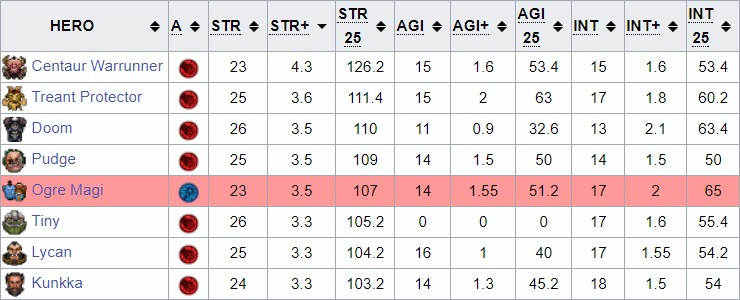
\includegraphics[scale=0.53]{img/centa.jpg}
	\caption{\textit{Stats} pada \textit{hero} Centaur.}
	\label{fig:centa}
\end{figure}

Dalam kasus ini diambil contoh Centaur, hero tersebut adalah bertipe STR, jika dilihat nilai \textit{Base} STR dan STR \textit{Growth} pada \textit{hero} ini sangat tinggi, namun ada cukup banyak hero lain yang mempunyai nilai \textit{stats} tinggi pada salah satu atribut tapi bukan merupakan \textit{hero} dengan tipe tersebut. Seperti Ogre Magi, \textit{hero} tersebut adalah type INT, tapi memililki nilai \textit{Base} STR, STR \textit{Growth} dan Max STR lebih tinggi dari pada \textit{stats} \textit{intelligent} seperti yang terlihat pada Gambar \ref{fig:centa}. 
\vspace{1ex}

Maka hal yang akan dilakukan disini adalah mencoba melakukan klasifikasi \textit{hero} berdasarkan \textit{stats} yang ada, dataset dari \textit{hero} Dota 2 dapat dilihat pada Tabel \ref{tb:dota2_hero_pt1} dan \ref{tb:dota2_hero_pt2} untuk data \textit{training} dan Tabel \ref{tb:dota2_hero_pt3} untuk data \textit{testing}. Selanjutnya adalah tahapan klasifikasinya seperti yang direpresentasikan pada Gambar \ref{fig:dota2_class_proc}.
\vspace{1ex}

\begin{figure} [!h] \centering
	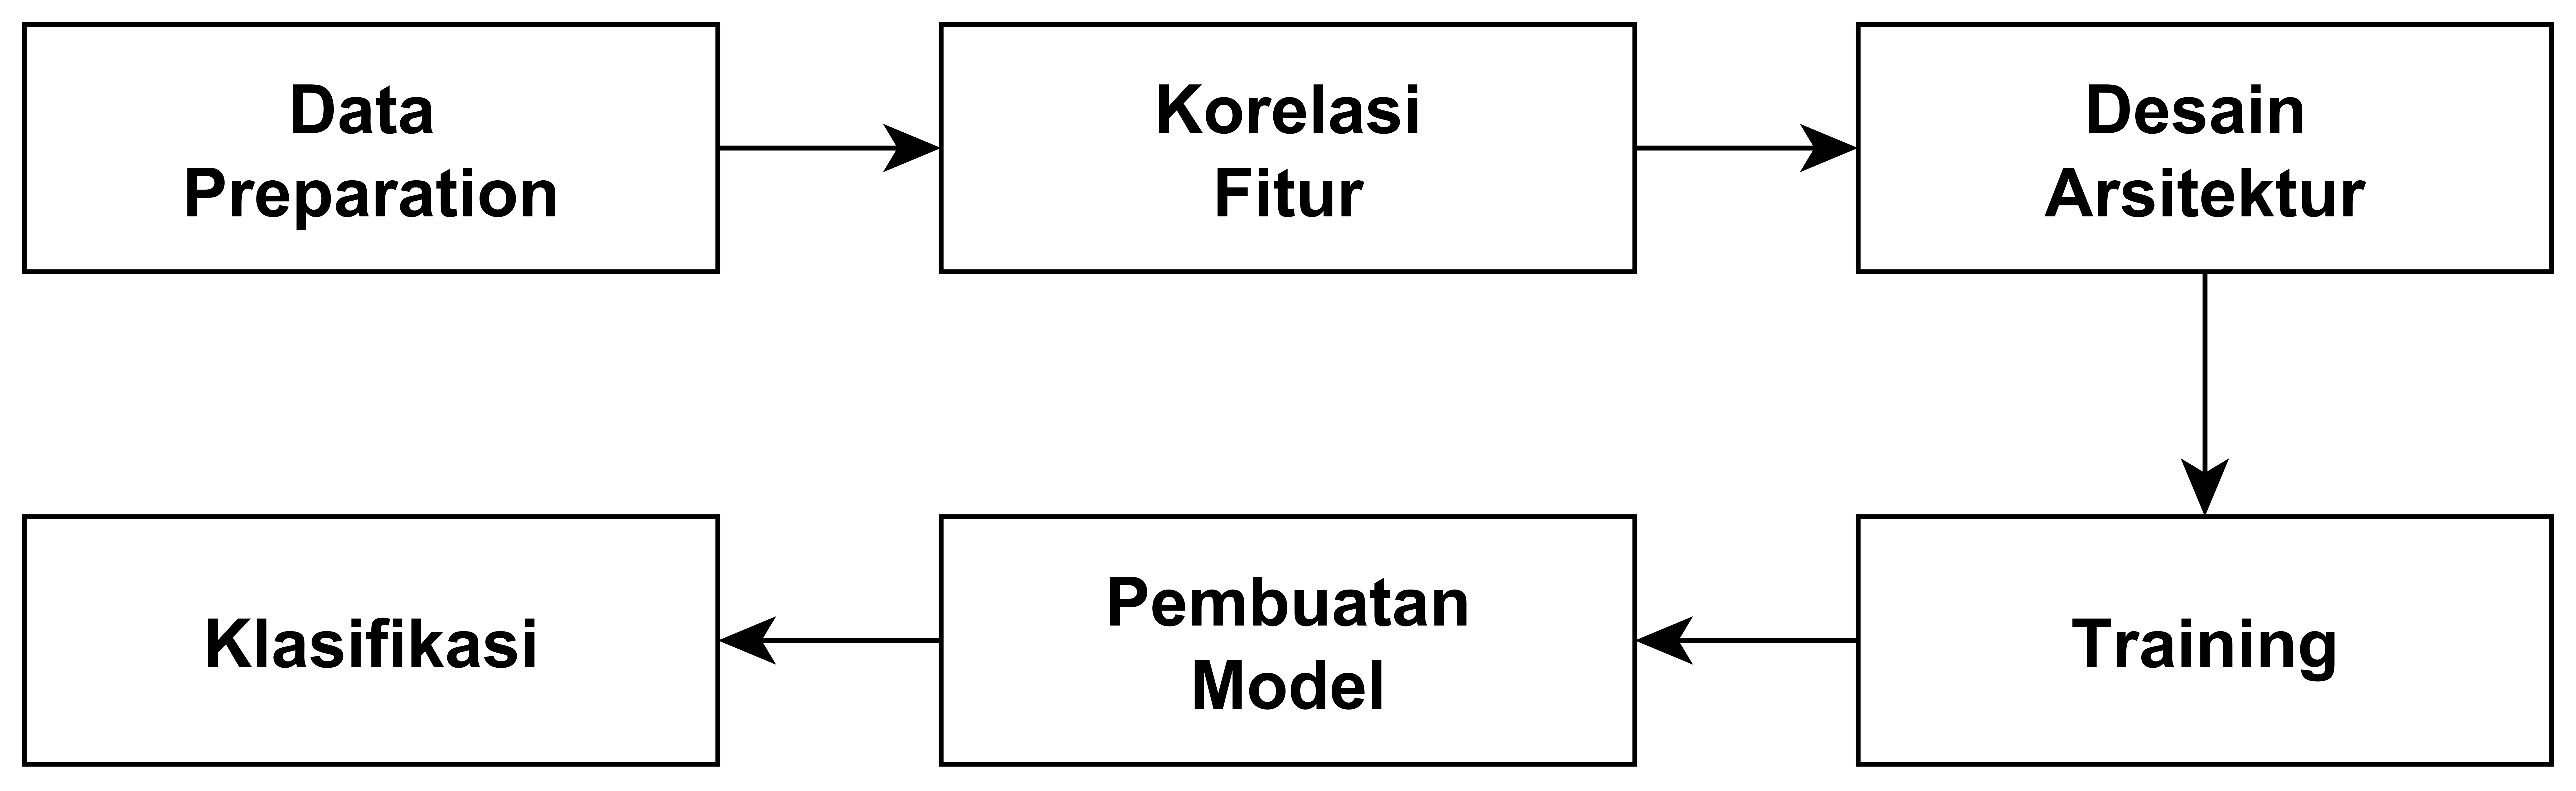
\includegraphics[scale=0.032]{img/dota2_nn_classification.png}
	\caption{Proses klasifikasi \textit{hero} pada permainan Dota 2.}
	\label{fig:dota2_class_proc}
\end{figure}

\subsection{Data Pre-processing}
\label{sec:sub_sec3_dota2_pre_proc}
\vspace{1ex}

Di lakukan \textit{parsing} halaman tersebut \citep{dota2020} dan dilakukan konversi dari tabel HTML menjadi CSV. Maka diperolehlah 115 buah data. Jika melihat Gambar \ref{fig:dota2_gameplay} terdapat beberapa data yang sifatnya spesifik untuk interaksi pada \textit{hero} tersebut didalam permainan. Hal tersebut ikut tercantum dalam dataset, maka akan dibuang, karena dianggap kurang relevan seperti \textit{Day Vision}, \textit{Night Vision}, \textit{Collision Size}, dan \textit{Legs}. Sehingga diperoleh 22 fitur yang akan digunakan untuk melakukan klasifikasi. Tipe \textit{hero} akan digunakan sebagai target dikategorikan dalam bentuk angka menjadi 0 untuk STR, 1 untuk AGI dan 2 untuk INT.
\vspace{1ex}

\begin{figure} [!h] \centering
	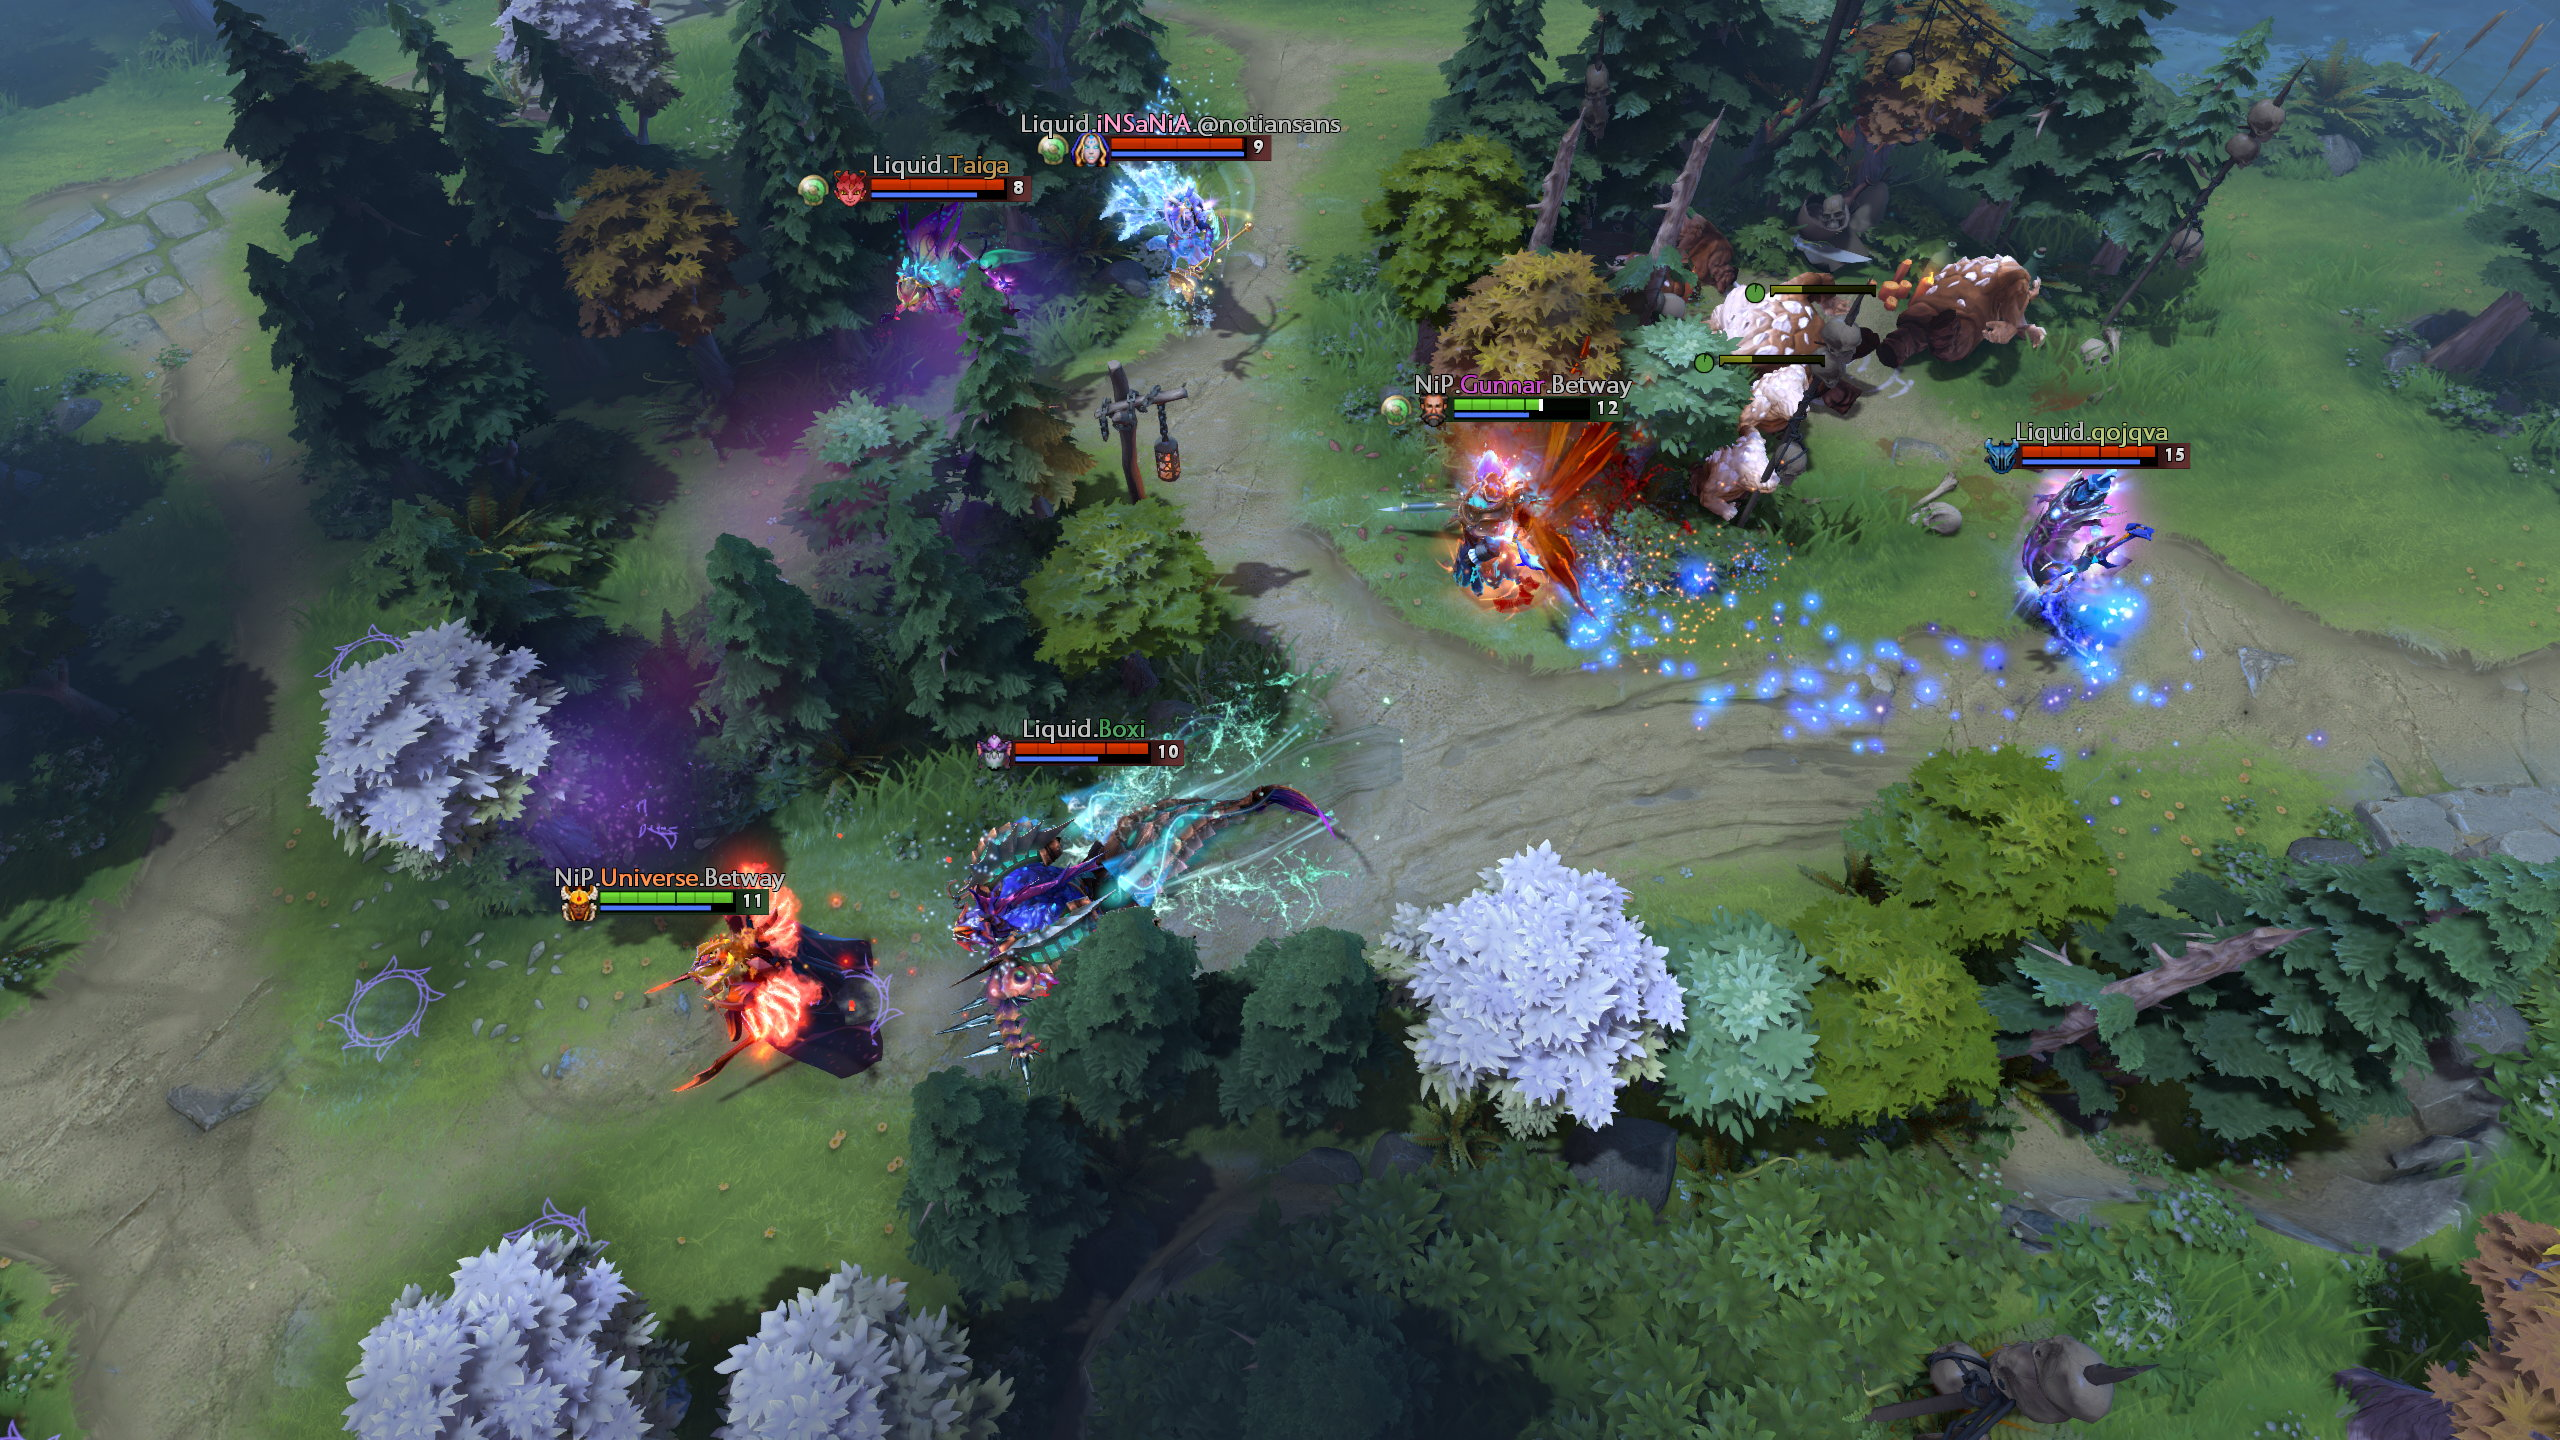
\includegraphics[scale=0.13]{img/dota2_gameplay.jpg}
	\caption{Proses klasifikasi \textit{hero} pada permainan Dota 2.}
	\label{fig:dota2_gameplay}
\end{figure}

Dari seluruh data \textit{hero} tersebut, enam belas \textit{hero} nantinya akan diambil sebagai data \textit{testing} yang tercantum pada Tabel \ref{tb:dota2_hero_pt3} dan sisanya digunakan sebagai data \textit{training} pada Tabel \ref{tb:dota2_hero_pt1} dan Tabel \ref{tb:dota2_hero_pt2} yang semua terlampir dalam \nameref{chap:chap6_attachment}. Untuk data \textit{testing} pada Tabel \ref{tb:dota2_hero_pt3}, diambilah beberapa \textit{hero} yang memiliki \textit{stats} aneh seperti Jakiro, Winter Wyvern (STR tinggi tetapi masuk ke dalam kategori INT \textit{hero}), Phoenix, IO (STR rendah tetapi termasuk ke dalam kategori STR hero), Bloodseeker, Undying, dan lain-lain.
\vspace{1ex}

\subsection{Korelasi Fitur}
\label{sec:sub_sec3_dota2_feature_corel}
\vspace{1ex}

Dari 22 fitur yang dibahas pada Sub-bab \ref{sec:sub_sec3_dota2_pre_proc}, bisa jadi tidak semua fitur mempunyai kontribusi terhadap tipe \textit{hero} atau bisa dibilang proses naik-turun sebuah fitur tersebut tidak memberikan pengaruh terhadap proses klasifikasi tipe \textit{hero}. Dalam pencarian fitur tersebut digunakanlah \textit{korelasi matrix} pada setiap variabel, hasil perhitungan korelasi matrix dari \textit{stats} Dota 2 yang dijadikan fitur dapat dilihat pada Tabel \ref{tb:dota2_matrix_corel}.
\vspace{-1ex}

\begin{longtable}{|l|l|}
	\caption{Hasil perhitungan korelasi matrix untuk fitur}
	\vspace{1ex}
	\label{tb:dota2_matrix_corel}\\
	\hline
	\rowcolor[HTML]{C0C0C0} 
	\textbf{Fitur} & \textbf{Korelasi Matrix} \\ \hline
	\textbf{type} & 1.000000 \\ \hline
	\textbf{baseStr} & -0.542666 \\ \hline
	\textbf{strGrowth} & -0.542322 \\ \hline
	\textbf{maxStr} & -0.581514 \\ \hline
	\textbf{baseAgi} & -0.038086 \\ \hline
	\textbf{agiGrowth} & -0.123072 \\ \hline
	\textbf{maxAgi} & -0.110488 \\ \hline
	\textbf{baseInt} & 0.688410 \\ \hline
	\textbf{intGrowth} & 0.657814 \\ \hline
	\textbf{maxInt} & 0.699666 \\ \hline
	\textbf{totalBaseAttr} & 0.179483 \\ \hline
	\textbf{totalAttrGrowth} & 0.063110 \\ \hline
	\textbf{totalMaxAttr} & 0.114713 \\ \hline
	\textbf{moveSpeed} & 0.067136 \\ \hline
	\textbf{baseArmor} & -0.113657 \\ \hline
	\textbf{minDmg} & -0.384719 \\ \hline
	\textbf{maxDmg} & -0.312799 \\ \hline
	\textbf{range} & 0.687704 \\ \hline
	\textbf{baseAttackTime} & -0.297982 \\ \hline
	\textbf{attackPoint} & -0.106053 \\ \hline
	\textbf{attackBackswing} & 0.011558 \\ \hline
	\textbf{turnRate} & -0.034759 \\ \hline
	\textbf{regeneration} & -0.090677 \\ \hline
\end{longtable}

Berikut penjelasan sederhana mengenai \textit{korelasi matrix}, hal tersebut membahas tentang sebuah variabel yang memuat nilai antara $-1$ dan $+1$. Sebagai contoh jika ada korelasi antara variabel $X$ dan $Y$ yang benilai $-1$, maka pada saat nilai $X$ turun, nilai $Y$ akan naik. Jika bernilai $+1$, maka hubungan antara $X$ dan $Y$ adalah linear. Namun jika nilai korelasi semakin dekat dengan $0$, maka variabel tersebut bisa dikatakan tidak mempengaruhi satu dengan yang lain.
\vspace{1ex}

Selanjutnya akan dibuang semua fitur yang memiliki nilai korelasi lebih kecil dari $0.1$ atau $-0.1$ seperti \textit{regeneration rate}, \textit{turn rate}, \textit{movement speed} dan yang paling aneh adalah fitur \textit{base} AGI, AGI \textit{growth} dan \textit{max} AGI memiliki nilai yang sangat kecil. Padahal fitur tersebut adalah termasuk kemampuan dasar dari \textit{hero}, sehingga didapatkan 16 fitur yang akan digunakan sebagai masukan untuk \textit{Neural Network}.
\vspace{1ex}

\subsection{Desain Arsitektur Neural Network}
\label{sec:sub_sec3_dota2_arch}
\vspace{1ex}

Arsitektur \textit{Neural Network} yang akan dibuat mempunyai enam belas \textit{neuron} pada layer masukan, delapan belas \textit{neuron} pada \textit{hidden layer} dengan fungsi aktivasi \textit{sigmoid} dan tiga \textit{neuron} yang mewakili (STR, AGI dan INT) pada layer keluaran seperti pada Gambar \ref{fig:nn_dota2} dengan fungsi aktivasi \textit{Softmax} karena keluaran dari model yang dibuat bersifat distribusi probabilitas dari seluruh nilai target. 
\vspace{1ex}

\begin{figure} [!h] \centering
	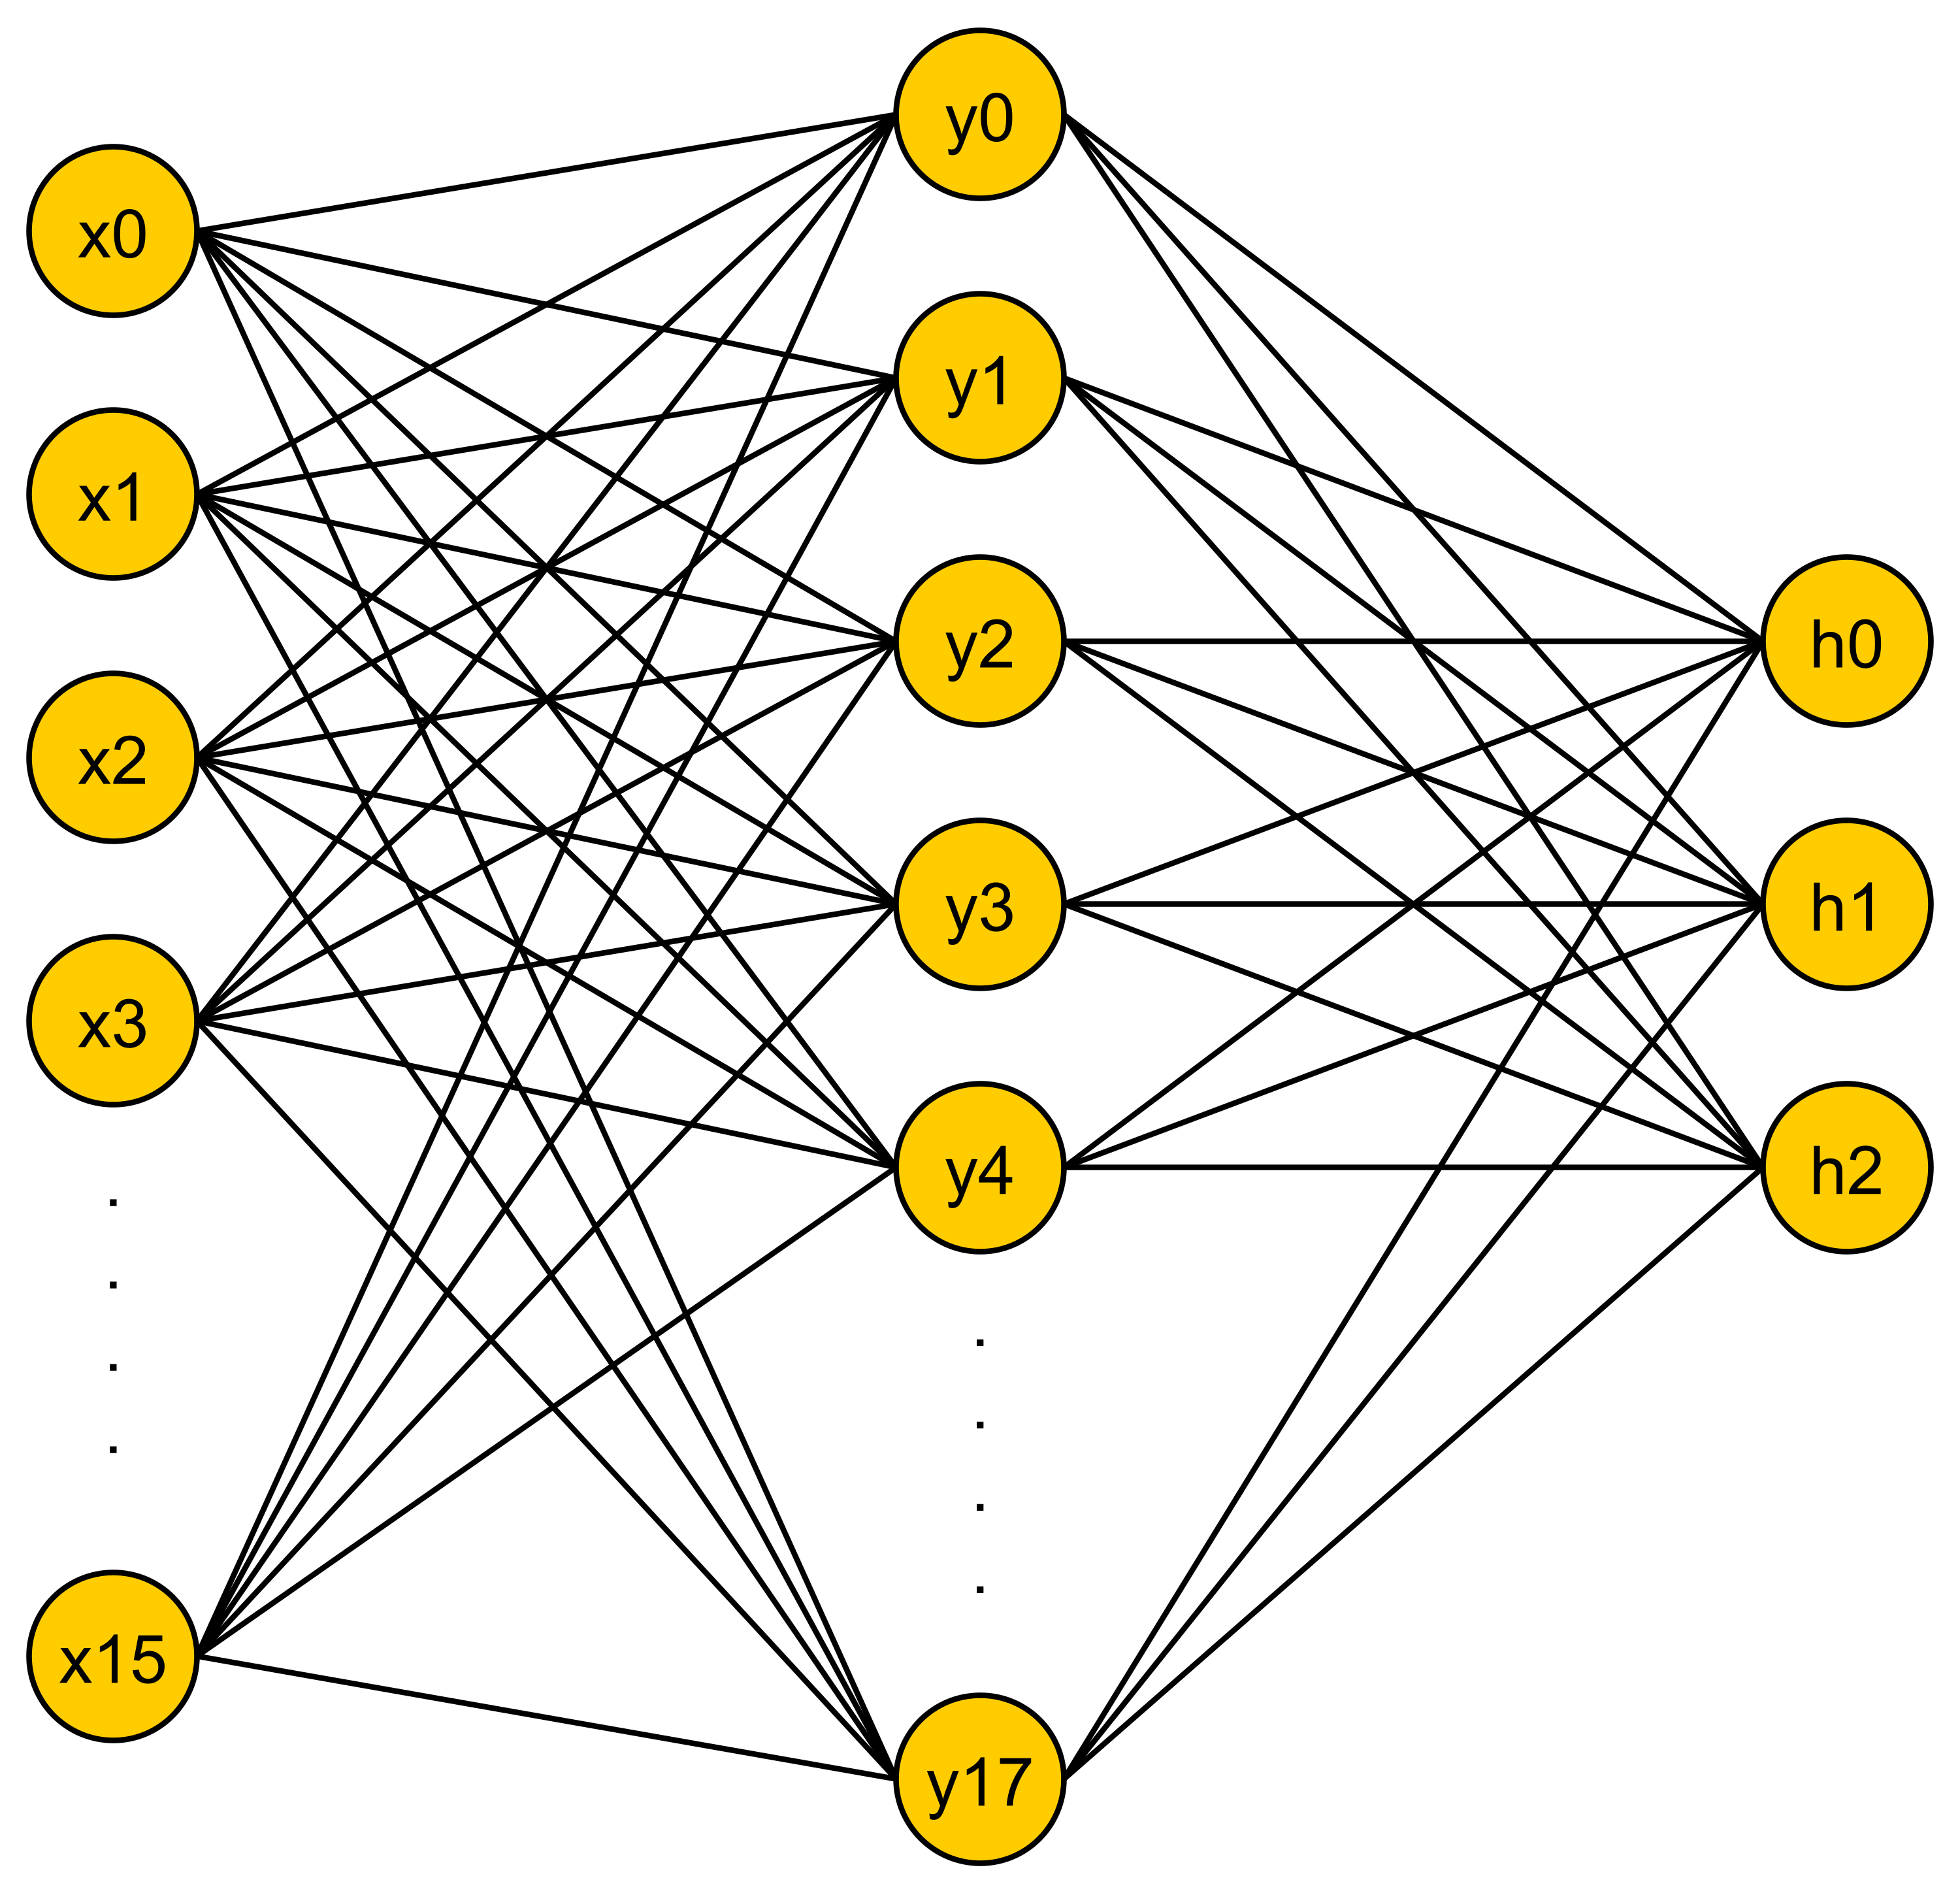
\includegraphics[scale=0.075]{img/nn_dota2.png}
	\caption{Arsitektur \textit{Neural Network} untuk klasifikasi \textit{hero} Dota 2.}
	\label{fig:nn_dota2}
\end{figure}

Misalkan model 100\% yakin jika \textit{hero} A adalah STR, maka keluaran dari model adalah $\left[1,\ 0,\ 0 \right]$ dan jika model tersenut 50\% yakin jika \textit{hero} B adalah AGI, 25\% yakin jika hero B adalah STR atau INT, maka keluaran dari model ini adalah $\left[0.25,\ 0.5,\ 0.25 \right]$. Harus diingat bahwa total nilai dari distribusi probabilitas untuk semua target adalah 1.
\vspace{1ex}

Sedangkan untuk \textit{loss function} yang digunakan adalah \textit{Cross Entropy} dan \textit{Optimizer} yang digunakan adalah SGD (\textit{Stochasstic Gradient Descent}) dengan \textit{learning rate} sebesar 0.001. Sebagai catatan penambahkan \textit{metrics accuracy} bertujuan untuk melihat seberapa bagus model ini dalam melakukan klasifikasi.
\vspace{1ex}

\subsection{Training}
\label{sec:sub_sec3_dota2_train}
\vspace{1ex}

Data hasil dari korelasi fitur pada Sub-bab \ref{sec:sub_sec3_dota2_feature_corel}, karena tipe yang ditunjukan pada kolom ke satu dengan kepala yang bertuliskan ``Fitur'' adalah pedoman hasil prediksi maka tidak akan diikutkan proses \textit{training}. Pada kolom \textit{type} tipe karakter dinyatakan dengan 0, 1, dan 2 yang menyatakan STR, AGI, dan INT. Nantinya keluaran dari hasil \textit{training} yang menunjukan prediksi tipe dari karakter dinyatakan dalam bentuk \textit{one-hot vector}: STR $\rightarrow [1, 0, 0]$, AGI $\rightarrow [0, 1, 0]$ dan INT $\rightarrow [0, 0, 1]$. 
\vspace{1ex}

Pada proses \textit{training} hasil prediksi akan dibandingkan dengan data \textit{testing} untuk mendapatkan nilai \textit{loss}/\textit{error} dan validasi untuk melihat performa model \textit{Neural Network} yang dibuat. Nilai \textit{loss} kemudian digunakan untuk meningkatkan akurasi model. Proses \textit{training} dilakukan untuk mendapatkan model dengan akurasi optimal dan tidak \textit{overfitting}.
\vspace{1ex}

Penentuan nilai \textit{batch size} dan \textit{learning rate} berperan penting dalam peningkatan akurasi hal ini biasa disebut dengan \textit{hyperparameter tuning}. Dengan \textit{Batch size} yang besar akan dapat memberikan jenis data yang bervariasi sehingga saat dilakukan perhitungan \textit{loss}, nilai perhitungan \textit{loss} yang diperoleh dapat mewakili variasi dataset secara keseluruhan. Sebaliknya \textit{batch size} yang kecil hanya dapat memberikan perwakilan sedikit dataset sehingga nilai perubahan \textit{loss} untuk memperoleh nilai yang stabil akan semakin sulit. Karena itu \textit{batch size} yang besar dapat diberikan \textit{learning rate} yang besar karena arah perpindahan \textit{loss} yang lebih stabil. Sedangkan \textit{batch size} yang kecil harus diberikan \textit{learning rate} yang kecil juga agar perpindahannya tidak berpindah pindah terlalu jauh.
\vspace{1ex}

Proses \textit{training} akan dilakukan sebanyak $2 \times 10^{4}$ \textit{epoch}/iterasi. Untuk satu \textit{epoch} dataset akan dibagi menjadi 16 \textit{batch size} tiap \textit{batch} hingga semua data terproses. Nilai \textit{learning rate} sebesar $1 \times 10^{-3}$ dan jika nilai \textit{loss} tidak mengalami perubahan maka \textit{learning rate} akan diperkecil sampai dengan $1 \times 10^{-4}$ seperti pada Gambar \ref{fig:nn_dota2_lr}. Namun dalam kasus ini digunakannya optimasi untuk menurunkan \textit{learning rate} saat nilai \textit{loss} tidak terjadi penurunan dan pemberhentian proses \textit{training} tanpa menunggu keseluruhan \textit{epoch} selesai. Pada Gambar \ref{fig:nn_dota2_val_loss_20k} adalah hasil \textit{training} tanpa menggunakan perubahan learning rate secara otomatis, sedangkan pada Gambar \ref{fig:nn_dota2_val_loss_callback} adalah hasil \textit{training} dengan perubahan \textit{learning rate} otomatis.

\begin{figure} [!htb] \centering
	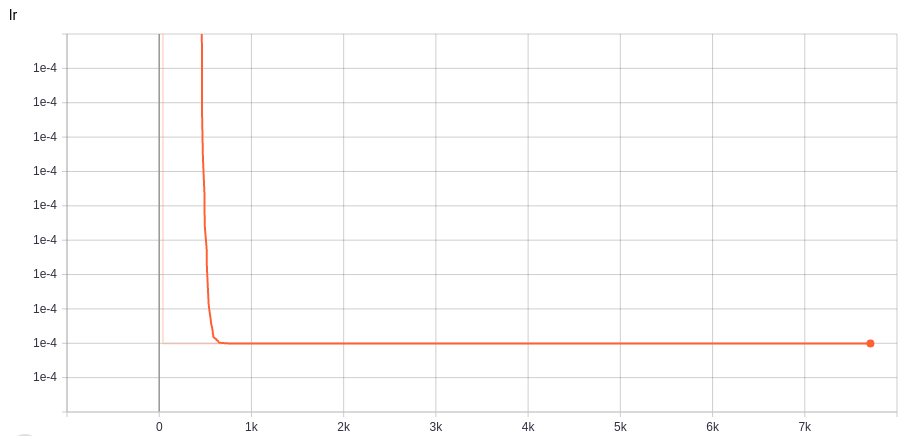
\includegraphics[scale=0.4]{img/callback_lr_chap3.png}
	\caption{Proses pengurangan \textit{learning rate} saat \textit{training}.}
	\label{fig:nn_dota2_lr}
\end{figure}

\begin{figure} [!htb] \centering
	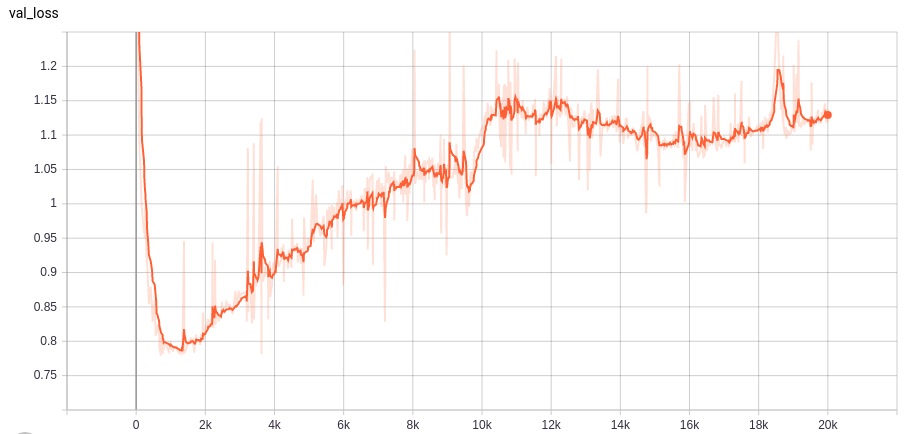
\includegraphics[scale=0.4]{img/hyperparam_val_loss_chap3.png}
	\caption{Validasi \textit{loss} saat $2 \times 10^{4}$ \textit{epoch}.}
	\label{fig:nn_dota2_val_loss_20k}
\end{figure}

\begin{figure} [!htb] \centering	
	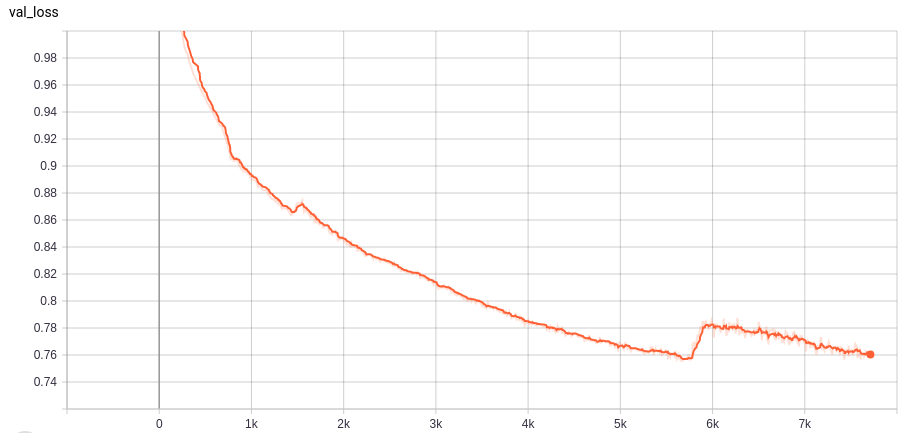
\includegraphics[scale=0.4]{img/callback_val_loss_chap3.png}
	\caption{Validasi \textit{loss} dengan pemberhentian otomatis.}
	\label{fig:nn_dota2_val_loss_callback}
\end{figure}

Pemberhentian proses \textit{training} tersebut dilakukan bukan tanpa alasan, jika terjadi kenaikan \textit{loss} khususnya pada proses validasi yang rawan terjadi kenaikan \textit{loss} atau \textit{loss validation} seperti pada Gambar \ref{fig:nn_dota2_val_loss_20k}. Saat terjadinya kenaikan \textit{loss} juga diberikan toleransi sebesar 1500 \textit{epoch}, hal tersebut bertujuan untuk mendeteksi apakah dalam \textit{range} 1500 \textit{epoch} akan terjadi penurunan \textit{loss} yang lebih kecil dari sebelumnya. Jika tidak terjadi penurunan dalam kurun 1500 \textit{epoch} tersebut, maka proses \textit{training} akan dihentikan seperti pada Gambar \ref{fig:nn_dota2_val_loss_callback}. Dapat dilihat pada Gambar \ref{fig:nn_dota2_val_loss_callback} \textit{training} dihentikan pada \textit{epoch} antara $7 \times 10^{3}$ dan $8 \times 10^{3}$.
\vspace{1ex}

\subsection{Pembuatan Model}
\label{sec:sub_sec3_dota2_model}
\vspace{1ex}

Model yang dihasilkan dari proses \textit{training} pada Sub-bab \ref{sec:sub_sec3_dota2_train} dapat digunakan untuk menguji atau menampilkan hasil klasifikasi pada data \textit{testing}, hasil tersebut akan ditampilkan dan dibahas pada Sub-bab \ref{sec:sec4_eval_dota2}. Pada Sub-bab ini akan lebih membahas mengenai model terbaik yang dihasilkan dari proses \textit{training}. Melanjutkan pembahasan sebelumnya pada Sub-bab \ref{sec:sec4_eval_dota2} tentang \textit{training} yang telah dilakukan meliputi penurunan \textit{learning rate}, pemberhentian \textit{training}, toleransi \textit{epoch} saat tidak terjadinya penurunan \textit{learing rate} dan yang paling berkataitan dengan Sub-bab ini pengambilan model terbaik. Pengambilan tersebut dilakukan pada saat \textit{epoch} dikurangi dengan 1500, dengan asumsi model terbaik diperoleh saat presentase \textit{validation loss} paling rendah dan 1500 tersebut adalah toleransi \textit{epoch}. Selama 1500 \textit{epoch} tersebut, kemudian \textit{training} berhenti, berarti tidak ditemukannya \textit{validation loss} yang lebih rendah dalam \textit{range} 1500 \textit{epoch} tersebut.
\vspace{1ex}

\section{Klasifikasi Karakter Pemain dengan Neural Network Multiclass Classification}
\label{sec:sec3_player_method}
\vspace{1ex}

Terdapat banyak sekali jenis permainan RPG seperti yang sudah dijelaskan pada Sub-bab \ref{sec:sec2_rpg}, tidak semua karakter yang dapat dimainkan oleh pemain berjumlah sangat banyak. Hanya beberapa genre RPG saja yang dapat menggunakan karakter pemain dengan jumlah sangat banyak. Jika mengacu genre permainan pada Sub-bab \ref{sec:sec2_rpg} dan judul permainan dijumpai saat ini permainan dengan genre JRPG dan MMORPG yang memungkinkan untuk memainkan banyak karakter dari pemain.
\vspace{1ex}

Pada pembahasan sebelumnya pada Sub-bab \ref{sec:sec3_dota2_method}, Dota 2 adalah permainan dengan genre MOBA (\textit{Multiplayer Online Battle Arena}) dengan beraneka karakter yang masing-masing dapat dipilih dan dimainkan oleh pemain. Jika dibandingkan dengan RPG yang dibahas pada Sub-bab \ref{sec:sec2_rpg}, mungkin RPG dengan banyak karakter yang dapat dilakukan proses klasifikasi. Maka genre yang memungkinkan dilakukan proses klasifikasi adalah JRPG, TRPG dan MMORPG dengan \textit{gameplay} yang mirip dengan JRPG. Sedangkan untuk WRPG, ARPG, SRPG, dan MMORPG dengan \textit{gameplay} karakter tunggal yang tidak mirip dengan JRPG atau TRPG.
\vspace{1ex}

Maka digunakanlah data masukan yang digunakan untuk membuat karakter pemain yang sebelumnya sudah dibahas pada Sub-bab \ref{sec:sec3_player_stats} pada Tabel \ref{tb:player_input_variable}. Data tersebut dibuat berdsarkan skenario seolah mendesain sebuah permainan. Pada permainan yang sebelumnya sempat dibahas pada Sub-bab \ref{sec:sec2_rpg} pasti terdapat juga karakter yang memiliki HP, \textit{strength} yang tinggi dan biasa diikuti dengan \textit{vitality} yang lumayan tinggi tetapi memiliki kecepatan atau \textit{agility} rendah. Kemudian mungkin terdapat juga karakter yang memiliki HP sedang, \textit{strength} yang rendah memiliki \textit{magic} dan \textit{agility} yang tinggi. Berikut adalah contoh skenario yang digunakan untuk mendesain karakter pemain berdasarkan tipe pada penelitian ini:

\begin{enumerate}[label=\arabic*).]
	\item Misalkan terdapat karakter dengan HP, \textit{strength} yang tinggi dan biasa diikuti dengan \textit{endurance} yang lumayan tinggi tetapi memiliki kecepatan atau \textit{agility} dan \textit{magic} rendah, maka dalam skenario ini dikategorikan sebagai \textbf{\textit{knight}} yang berfungsi sebagai penahan serangan dan bisa juga melakukan serangan. 
	
	\item Kemudian terdapat karakter yang memiliki \textit{strength} yang tidak begitu tinggi, tetapi memiliki \textit{endurance} yang cukup tinggi diikuti dengan \textit{magic} yang tinggi tetapi \textit{agility} rendah. Pada Skenario ini karakter tersebut adalah \textbf{\textit{priest}} yang bertugas untuk menyembuhkan \textit{party member} yang terluka atau mengalami pengurangan HP. 
	
	\item Karakter dengan \textit{agility} atau kecepatan dan ketepatan yang tinggi dengan tingkat \textit{luck} atau keberuntungan yang tinggi mengakibatkan berlipat gandanya \textit{strength} atau kekuatan saat melakukan serangan. Pada skenario ini, karakter tersebut adalah \textbf{\textit{assassin}} yang berperan sebagai penyerang dari \textit{party} yang dapat membunuh karakter musuh dengan cepat dengan kemampuan fisik.
	
	\item Terdapat juga karakter yang memiliki HP sedang, \textit{strength} yang rendah, mungkin dengan \textit{endurance} yang sedang juga, tetapi memiliki \textit{magic} dan \textit{agility} yang tinggi. Dalam skenario ini, karakter tersebut adalah \textbf{\textit{magician}} yang berperan sebagai penyerang dari \textit{party} dengan kemampuan \textit{magic}.
\end{enumerate}

Maka hal yang akan dilakukan disini adalah mencoba melakukan klasifikasi karakter berdasarkan \textit{stats} yang ada, dataset dari karakter pemain dapat dilihat pada Tabel \ref{tb:player_char_train} untuk data \textit{training} dan Tabel \ref{tb:player_char_test} untuk \textit{testing}. Selanjutnya adalah tahapan klasifikasinya seperti yang direpresentasikan pada Gambar \ref{fig:player_class_proc}. 
\vspace{1ex}

\begin{figure} [!h] \centering
	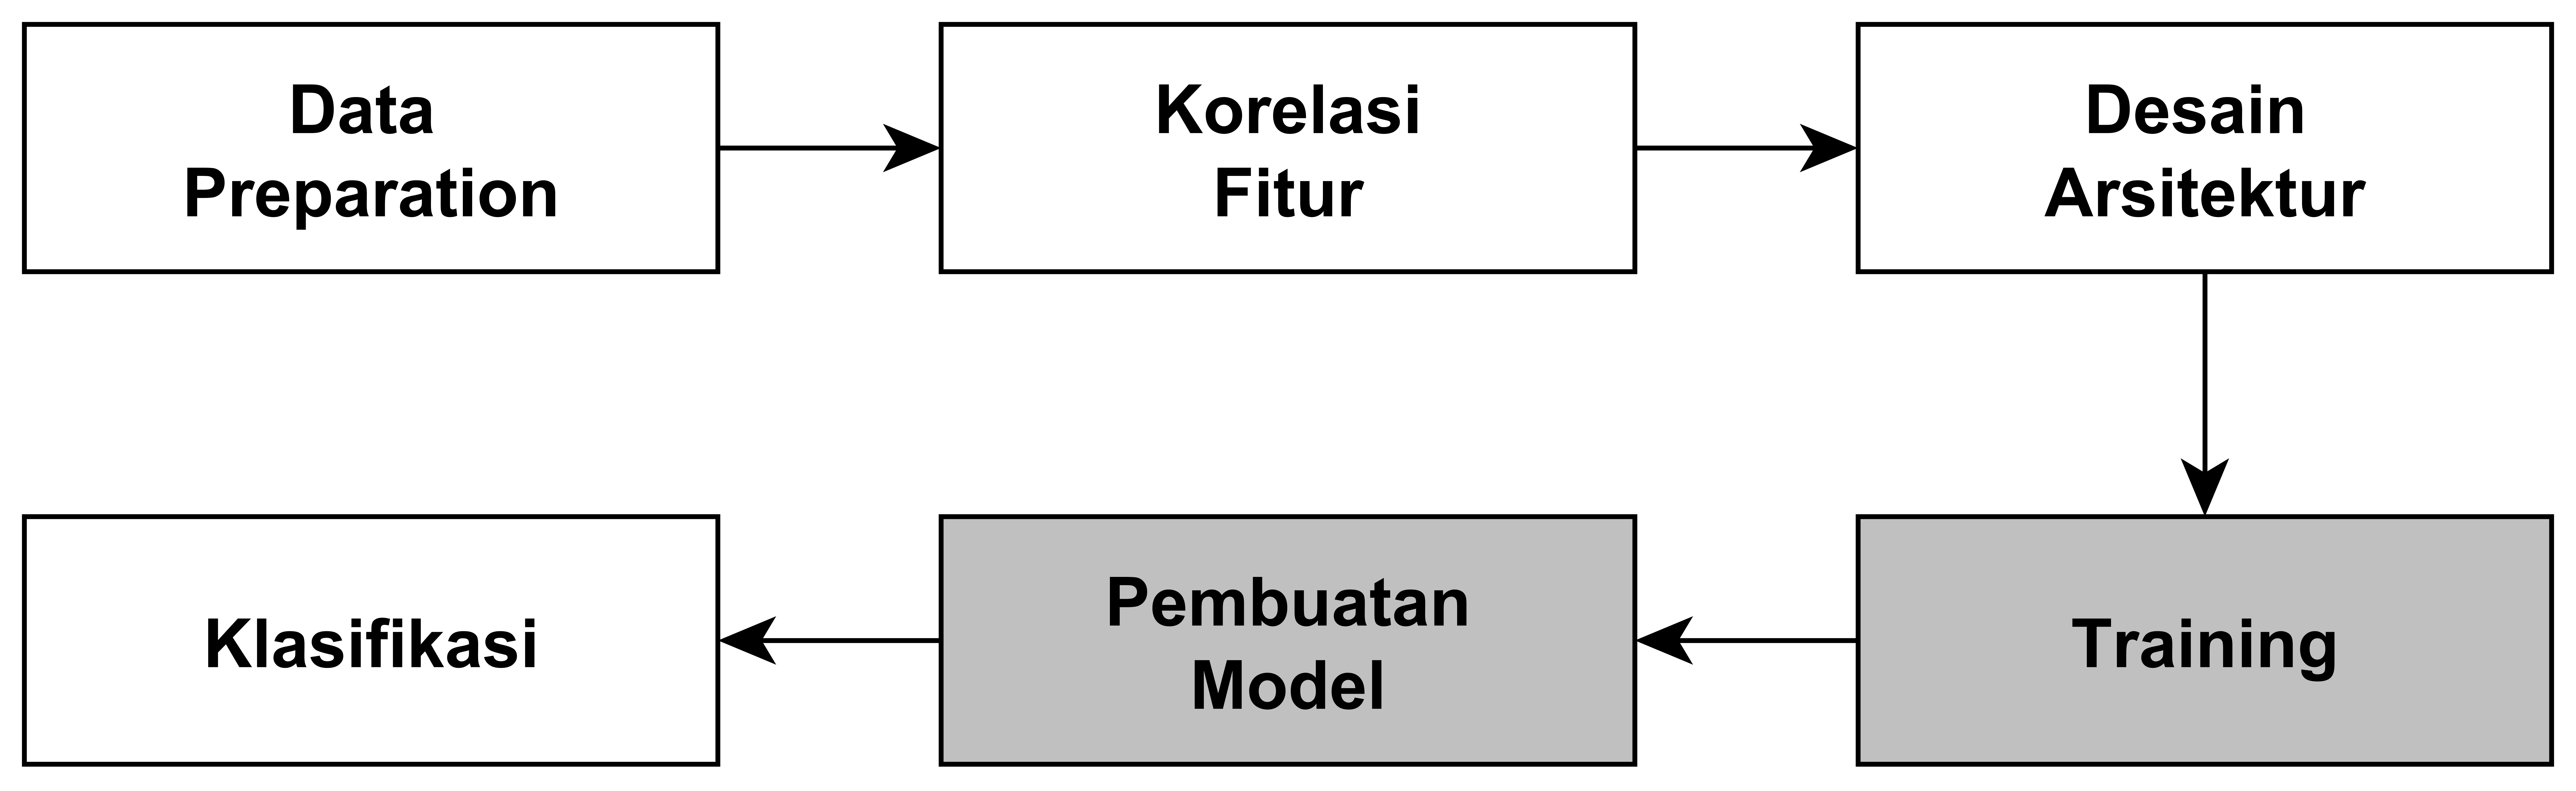
\includegraphics[scale=0.035]{img/player_char_nn_classification.png}
	\caption{Proses klasifikasi Karakter Pemain.}
	\label{fig:player_class_proc}
\end{figure}

Pada dasarnya Gambar \ref{fig:player_class_proc} mirip dengan Gambar \ref{fig:dota2_class_proc}, dikarenakan proses yang dilalui sama persis, hanya saja pada bagian proses \textit{training} dan pembuatan model yang ditandai dengan warna abu-abu penjelasannya akan banyak dilewati dikarenakan proses tersebut hampir sama dengan Gambar \ref{fig:dota2_class_proc} yang kemudian dijelaskan pada Sub-bab \ref{sec:sub_sec3_dota2_arch} dan Sub-bab \ref{sec:sub_sec3_dota2_model}. Kemudian pada Gambar \ref{fig:dota2_class_proc}, data \textit{pre-processing} diganti menjadi data \textit{preparation} dikarenakan data dibuat sesuai dengan masukan data dalam pembuatan karakter pemain yang sudah dijelaskan pada Sub-bab \ref{sec:sec3_player_stats}.
\vspace{1ex}

\subsection{Data Preparation}
\label{sec:sub_sec3_player_data_prep}
\vspace{1ex}

Dataset dari karakter pemain dapat dilihat pada Tabel \ref{tb:player_char_train} untuk data \textit{training} dan Tabel \ref{tb:player_char_test} untuk data \textit{testing}. Data tersebut diperoleh dari Tabel \ref{tb:player_input_variable} dengan kenaikan pada masing-masing variabel misalkan pada HP yang diawali dengan \textit{Start HP} yang kemudian akan naik sebesar \textit{Next HP} begitu juga dengan MP. Sedangkan untuk kenaikan \textit{stats} seperti \textit{Strength}, \textit{Magic}, \textit{Endurance}, \textit{Speed} dan \textit{Luck} diperoleh berdasarkan penambahan sejumlah variabel \textit{Stats to Assign} dangan hasil akhir sejumlah variabel \textit{Max Stats Value}. Bila dijabarkan dalam proses kenaikan \textit{stats} setiap level maka hasilnya akan seperti Tabel \ref{tb:player_all_stats_1} sampai dengan Tabel \ref{tb:player_all_stats_4} yang diperoleh dari proses yang dijelaskan pada Sub-bab \ref{sec:sec3_player_stats}, dan bila setiap kenaikan \textit{stats} dirata-rata maka hasilnya akan seperti data di baris pertama pada Tabel \ref{tb:player_char_train} terlampir dalam \nameref{chap:chap6_attachment}. 
\vspace{1ex}

Sedangkan untuk baris lain pada Tabel \ref{tb:player_char_train} dan Tabel \ref{tb:player_char_test} dibuat satu-satu dengan variabel masukan seperti pada Tabel \ref{tb:player_input_variable}, namun dengan nilai yang berbeda. Nilai tersebut menyesuaikan dengan skenario yang dijelaskan diawal Sub-bab \ref{sec:sec3_player_method}. Jumlah karakter pemain yang dibuat berjumlah 8 karakter yang dibagi menjadi 6 data \textit{training} dan 2 data \textit{testing}.  Kemudian untuk kelemahan dari pemain tidak diguanakan sebagai fitur, dikarenakan nilainya yang cenderung kurang bervariasi yang mengakibatkan akan semakin mendekati nol saat dilakukan korelasi fitur.
\vspace{1ex}

\subsection{Korelasi Fitur}
\label{sec:sub_sec3_player_feature_corel}
\vspace{1ex}

Dilakukan proses korelasi fitur seperti yang dilakukan pada Sub-bab \ref{sec:sub_sec3_dota2_feature_corel}, hanya saja kali ini data yang dikorelasi fitur berbeda dengan data sebelumnya. Jika data sebelumnya adalah \textit{stats} untuk permainan Dota 2, maka data yang digunakan adalah \textit{stats} dari karakter pemain seperti penjelasan pada paragraf sebelumnya. Hasil perhitungan korelasi fitur menggunakan korelasi matrix dari \textit{stats} karakter pemain dapat dilihat pada Tabel \ref{tb:player_matrix_corel}. Selanjutnya akan dibuang semua fitur yang memiliki nilai korelasi lebih kecil dari $0.1$, $-0.1$ dan $NaN$ seperti minStr atau \textit{minimum strength}, minMag atau \textit{minimum Magic}, minEnd atau \textit{minimum endurance}, minSpd atau \textit{minimum speed}, dan minLuck atau \textit{minimum luck}. Sehingga didapatkan 16 fitur yang akan digunakan sebagai masukan untuk \textit{Neural Network}.
\vspace{-1ex}

\begin{longtable}{|l|l|}
	\caption{Hasil perhitungan korelasi matrix pada data pemain}
	\vspace{1ex}
	\label{tb:player_matrix_corel}\\
	\hline
	\rowcolor[HTML]{C0C0C0}
	\textbf{Fitur} & \textbf{Korelasi Matix} \\ \hline
	\textbf{type} & 1.000000 \\ \hline
	\textbf{minHP} & -0.629568 \\ \hline
	\textbf{maxHp} & -0.678790 \\ \hline
	\textbf{hpGrowth} & -0.408248 \\ \hline
	\textbf{minMP} & 0.481794 \\ \hline
	\textbf{maxMp} & 0.619225 \\ \hline
	\textbf{mpGrowth} & 0.653197 \\ \hline
	\textbf{minStr} & NaN \\ \hline
	\textbf{maxStr} & -0.745061 \\ \hline
	\textbf{strGrowth} & -0.745061 \\ \hline
	\textbf{minMag} & NaN \\ \hline
	\textbf{maxMag} & 0.723322 \\ \hline
	\textbf{magGrowth} & 0.723322 \\ \hline
	\textbf{minEnd} & NaN \\ \hline
	\textbf{maxEnd} & -0.842417 \\ \hline
	\textbf{endGrowth} & -0.842417 \\ \hline
	\textbf{minSpd} & NaN \\ \hline
	\textbf{maxSpd} & 0.668815 \\ \hline
	\textbf{spdGrowth} & 0.668815 \\ \hline
	\textbf{minLuck} & NaN \\ \hline
	\textbf{maxLuck} & 0.338762 \\ \hline
	\textbf{luckGrowth} & 0.338762 \\ \hline
\end{longtable}
\vspace{1ex}

\subsection{Desain Arsitektur Neural Network}
\label{sec:sub_sec3_player_arch}
\vspace{1ex}

Arsitektur \textit{Neural Network} yang akan dibuat mempunyai enam belas \textit{neuron} pada layer masukan, delapan belas \textit{neuron} pada \textit{hidden layer} dengan fungsi aktivasi \textit{sigmoid} dan lima \textit{neuron} yang mewakili (\textit{Knight}, \textit{Priest}, \textit{Assassin}, dan \textit{Magician}) pada layer keluaran seperti pada Gambar \ref{fig:nn_player} dengan fungsi aktivasi \textit{Softmax} karena keluaran dari model yang dibuat bersifat distribusi probabilitas. Misalkan model kita 100\% yakin jika karakter A adalah \textit{Knight}, maka keluaran dari model adalah $\left[1,\ 0,\ 0,\ 0 \right]$ dan jika model kita 50\% yakin jika hero B adalah \textit{Priest}, 25\% yakin jika hero B adalah \textit{Knight} atau \textit{Magician}, maka output dari model ini adalah $\left[0.25,\ 0.5,\ 0.25, \ 0 \right]$. Harus diingat bahwa total nilai dari distribusi probabilitas untuk semua target adalah 1. Sedangkan untuk \textit{loss function} yang digunakan adalah \textit{Cross Entropy} dan \textit{Optimizer} yang digunakan adalah SGD (\textit{Stochasstic Gradient Descent}) dengan \textit{learning rate} sebesar 0.001. Sebagai catatan penambahkan \textit{metrics accuracy} bertujuan untuk melihat seberapa bagus model dalam melakukan klasifikasi.
\vspace{1ex}

\begin{figure} [!h] \centering
	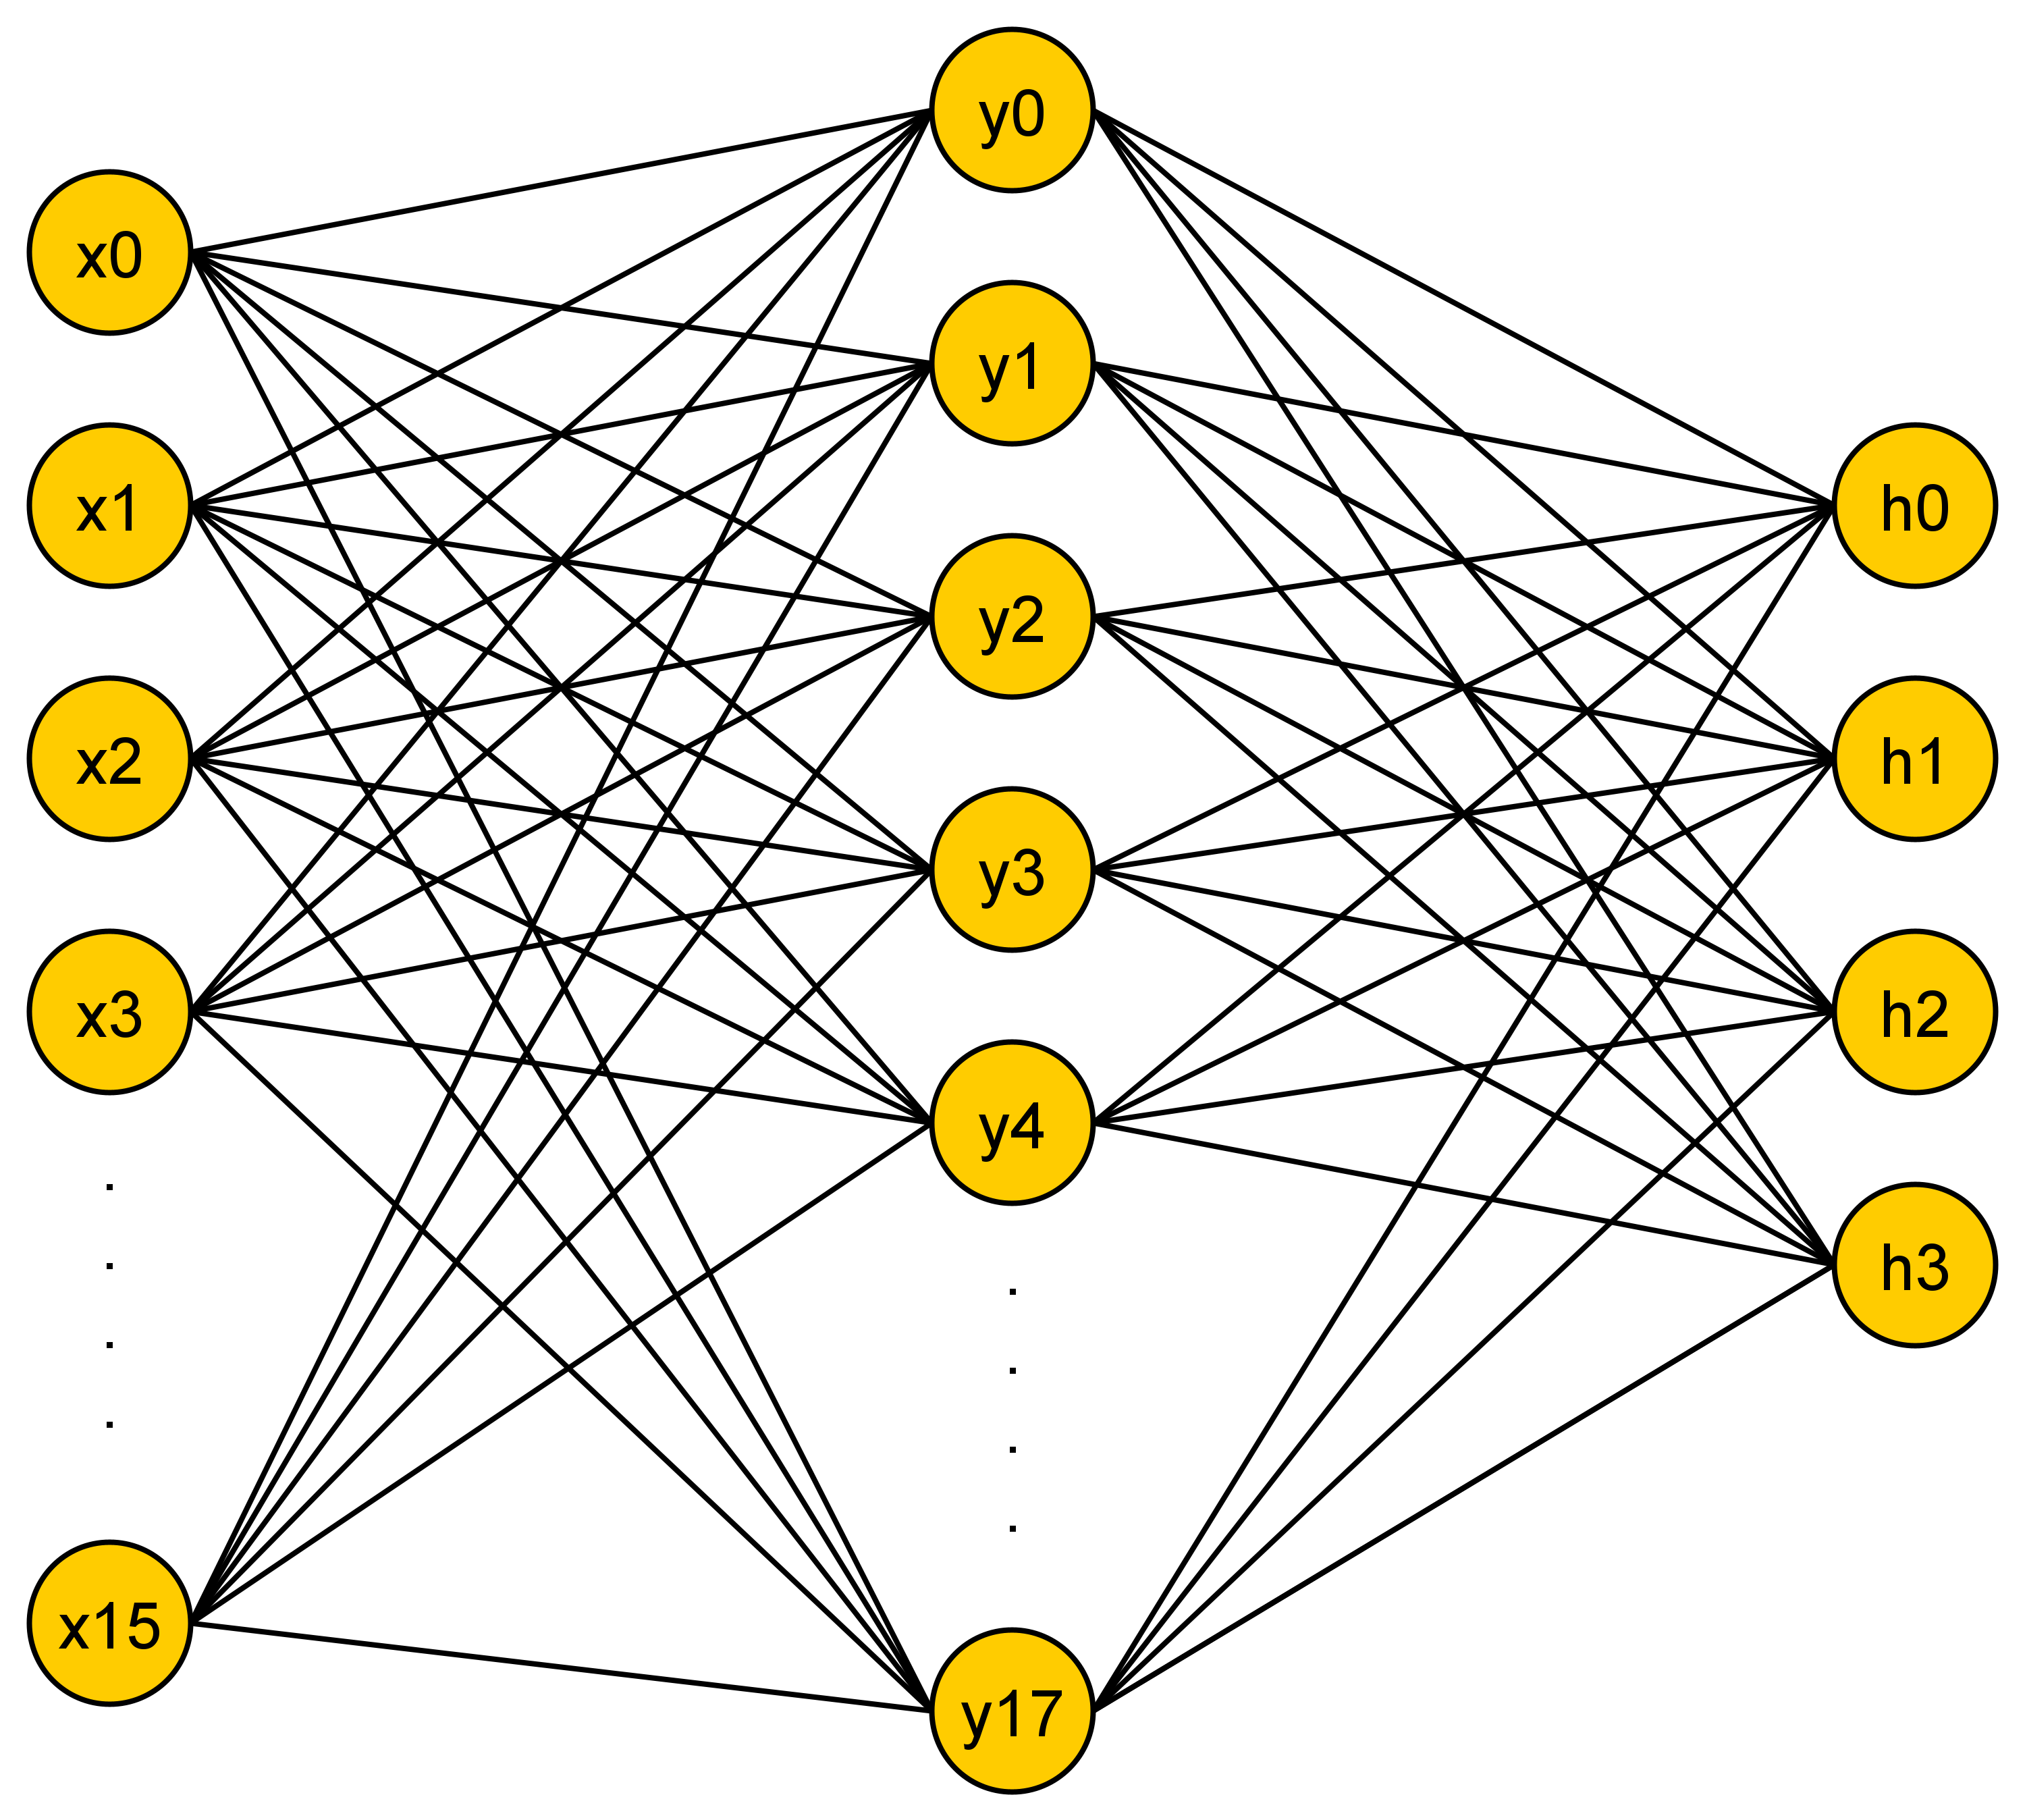
\includegraphics[scale=0.08]{img/nn_player_character.png}
	\caption{Arsitektur \textit{Neural Network} untuk klasifikasi karakter pemain.}
	\label{fig:nn_player}
	\vspace{1ex}
\end{figure}

\subsection{Training dan Pembuatan Model}
\label{sec:sub_sec3_player_char_train}
\vspace{1ex}

Data hasil dari korelasi fitur pada Sub-bab \ref{sec:sub_sec3_player_feature_corel}, karena tipe yang ditunjukan pada kolom ke satu dengan kepala bertuliskan ``Fitur'' adalah pedoman hasil prediksi maka tidak akan diikutkan proses \textit{training}. Pada kolom \textit{type} tipe karakter dinyatakan dengan 0, 1, 2, dan 3 yang menyatakan \textit{Knight}, \textit{Priest}, \textit{Assassin} dan \textit{Magician}. Nantinya keluaran dari hasil \textit{training} yang menunjukan prediksi tipe dari karakter dinyatakan dalam bentuk \textit{one-hot vector}: \textit{Knight} $\rightarrow [1, 0, 0, 0]$, \textit{Priest} $\rightarrow [0, 1, 0, 0]$, \textit{Assassin} $\rightarrow [0, 0, 1, 0]$ dan \textit{Magician} $\rightarrow [0, 0, 0, 1]$. Kemudian untuk optimasi dan pembuatan model sama seperti Sub-bab \ref{sec:sub_sec3_dota2_model}. Model yang dihasilkan dari proses \textit{training} pada Sub-bab \ref{sec:sub_sec3_player_char_train} dapat digunakan untuk menguji atau menampilkan hasil klasifikasi pada data \textit{testing} yang dibahas pada Sub-bab \ref{sec:sec4_eval_dota2}.
\vspace{1ex}

\section{Klasifikasi Karakter Musuh dengan Neural Network Multiclass Classification}
\label{sec:sec3_enemy_method}
\vspace{1ex}

Hal yang akan dilakukan disini adalah langsung melakukan klasifikasi karakter musuh berdasarkan \textit{stats} yang ada, dataset dari karakter musuh dapat dilihat pada Tabel \ref{tb:enemy_all_stats_1} sampai dengan Tabel \ref{tb:enemy_all_stats_15} untuk musuh dengan urutan ke 1 sampai 280 digunakan sebagai data \textit{training} dan Tabel \ref{tb:enemy_all_stats_1} sampai dengan Tabel \ref{tb:enemy_all_stats_15} untuk musuh dengan urutan ke 281 sampai paling akhir digunakan sebagai data \textit{testing}. Tanpa perlu adanya skenario dikarenakan jumlah musuh yang tentunya sudah sangat banyak dan bermacam-macam yang telah dibuat melalui serangkaian proses pada Sub-bab \ref{sec:sec3_enemy_stats}. Selanjutnya adalah tahapan klasifikasinya seperti yang direpresentasikan pada Gambar \ref{fig:enemy_class_proc}.
\vspace{1ex}

\begin{figure} [!h] \centering
	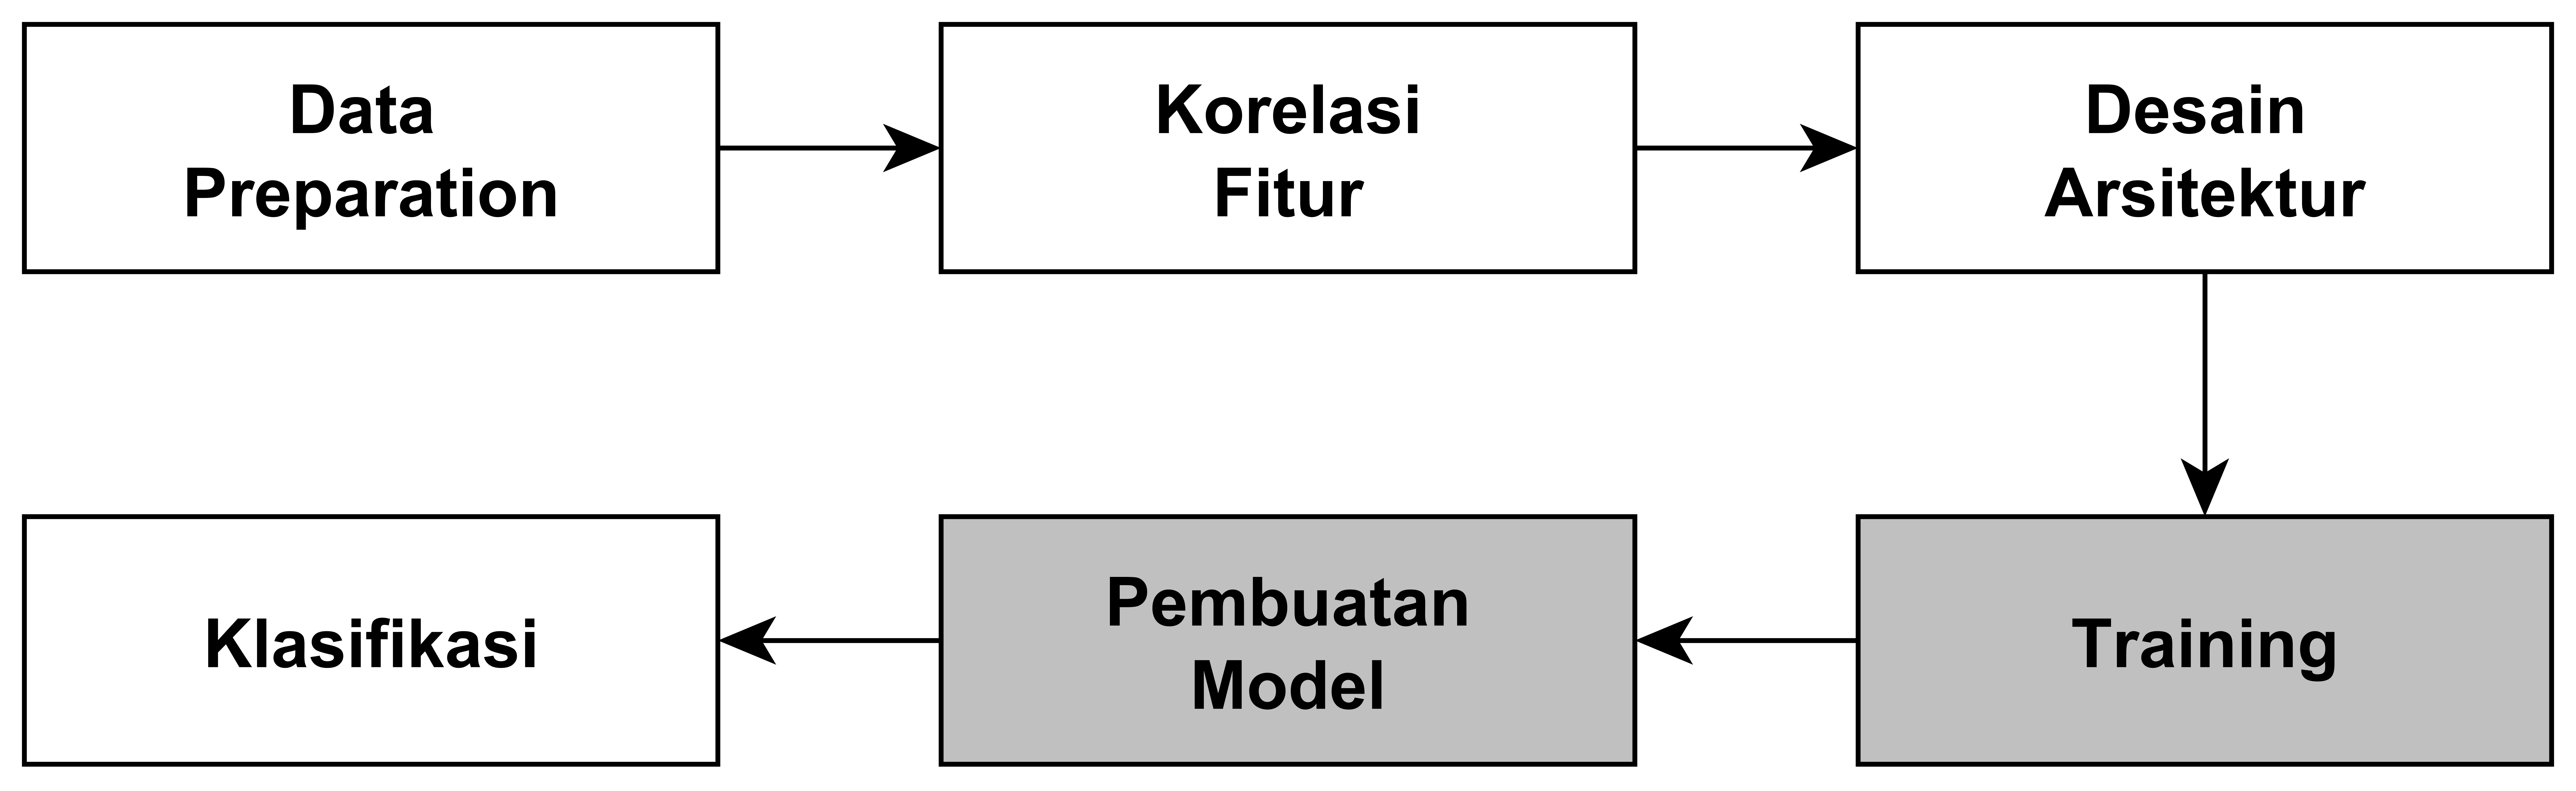
\includegraphics[scale=0.035]{img/player_char_nn_classification.png}
	\caption{Proses klasifikasi Karakter Musuh.}
	\label{fig:enemy_class_proc}
\end{figure}

Pada dasarnya Gambar \ref{fig:enemy_class_proc} mirip dengan Gambar \ref{fig:dota2_class_proc}, dikarenakan proses yang dilalui sama persis, hanya saja pada bagian proses \textit{training} dan pembuatan model yang ditandai dengan warna abu-abu karena penjelasannya akan banyak dilewati dikarenakan proses tersebut hampir sama dengan Gambar \ref{fig:dota2_class_proc} yang sudah dijelaskan pada Sub-bab \ref{sec:sub_sec3_dota2_arch} dan Sub-bab \ref{sec:sub_sec3_dota2_model}. Kemudian pada Gambar \ref{fig:dota2_class_proc}, data \textit{pre-processing} diganti menjadi data \textit{preparation} dikarenakan data dibuat secara manual sesuai dengan masukan data dalam membuat karakter pemain yang sudah dijelaskan pada Sub-bab \ref{sec:sec3_enemy_stats}.
\vspace{1ex}

\subsection{Data Preparation}
\label{sec:sub_sec3_enemy_data_prep}
\vspace{1ex}

Dataset dari karakter musuh dapat dilihat pada Tabel \ref{tb:enemy_all_stats_1} sampai dengan Tabel \ref{tb:enemy_all_stats_15} untuk musuh dengan urutan ke 1 sampai 280 digunakan sebagai data \textit{training} dan Tabel \ref{tb:enemy_all_stats_1} sampai dengan Tabel \ref{tb:enemy_all_stats_15} untuk musuh dengan urutan ke 281 sampai 400 digunakan sebagai data \textit{testing} dan \textit{testing}. Data tersebut diperoleh dari Tabel \ref{tb:enemy_input_variable} yang kemudian dijelaskan setiap proses pembuatan data tersebut pada Sub-bab \ref{sec:sec3_player_stats}. Kemudian untuk kelemahan dari musuh tidak diguanakan sebagai fitur sama seperti pada karakter pemain, hal tersebut dikarenakan nilainya yang cenderung kurang bervariasi yang mengakibatkan akan semakin mendekati nol saat dilakukan korelasi fitur.
\vspace{1ex}

Maka digunakanlah data masukan yang digunakan untuk membuat karakter musuh yang sebelumnya sudah dibahas pada Sub-bab \ref{sec:sec3_enemy_stats} pada Tabel \ref{tb:enemy_input_variable}. Data tersebut dibuat berdasarkan skenario seolah mendesain sebuah permainan. Pada permainan yang sebelumnya sempat dibahas pada Sub-bab \ref{sec:sub_sec3_story} pasti terdapat juga karakter musuh yang susah atau mudah dikalahkan, memiliki kemampuan \textit{magic} yang tinggi, sedang, atau rendah, memiliki kemampuan \textit{strength} yang tinggi, sedang, atau rendah, dan lain sebagainya. Berikut adalah contoh skenario yang digunakan untuk mendesain karakter musuh berdasarkan tipe pada penelitian ini:

\begin{enumerate}[label=\arabic*).]
	\item Misalkan terdapat karakter dengan HP, \textit{strength} yang sangat tinggi sampai dengan sedang dan biasa diikuti dengan \textit{endurance} juga tetapi memiliki kecepatan atau \textit{agility} dan \textit{magic} rendah, maka dalam skenario ini dikategorikan sebagai \textbf{\textit{Hard Strength}}. 
	
	\item Misalkan terdapat karakter dengan HP, \textit{strength} yang lumayan tinggi sampai dengan sedang dan biasa diikuti dengan \textit{endurance} juga tetapi memiliki kecepatan atau \textit{agility} dan \textit{magic} rendah, maka dalam skenario ini dikategorikan sebagai \textbf{\textit{Soft Strength}}.
	
	\item Misalkan terdapat karakter dengan \textit{strength} dari sedang sampai dengan rendah dan biasa diikuti dengan \textit{endurance} juga tetapi memiliki \textit{magic} yang sangat tinggi, maka dalam skenario ini dikategorikan sebagai \textbf{\textit{Hard Magic}}.
	
	\item Misalkan terdapat karakter dengan \textit{strength} dari sedang sampai dengan rendah dan biasa diikuti dengan \textit{endurance} juga tetapi memiliki \textit{magic} yang lumayan tinggi sampai dengan sedang, maka dalam skenario ini dikategorikan sebagai \textbf{\textit{Soft Magic}}.
	
	\item Misalkan terdapat karakter nilai \textit{stats} yang tidak menentu dengan \textit{strength} dari rendah sampai dengan tinggi, begitu juga dengan magic, namum dalam distribusi stats tetap seimbang. Maka dalam skenario ini dikategorikan sebagai \textbf{\textit{Mixed}}.
\end{enumerate}

\subsection{Korelasi Fitur}
\label{sec:sub_sec3_enemy_feature_corel}
\vspace{1ex}

Dilakukan proses korelasi fitur seperti yang dilakukan pada Sub-bab \ref{sec:sub_sec3_dota2_feature_corel}, hanya saja kali ini data yang dikorelasi fitur berbeda dengan data sebelumnya. Jika data sebelumnya adalah \textit{stats} untuk permainan Dota 2, maka data yang digunakan adalah \textit{stats} dari karakter musuh seperti penjelasan pada paragraf sebelumnya. Hasil perhitungan korelasi fitur menggunakan korelasi matrix dari \textit{stats} karakter pemain dapat dilihat pada Tabel \ref{tb:enemy_matrix_corel}.
\vspace{-1ex}

\begin{longtable}{|l|l|}
	\caption{Hasil perhitungan korelasi matrix pada data musuh}
	\vspace{1ex}
	\label{tb:enemy_matrix_corel}\\
	\hline
	\rowcolor[HTML]{C0C0C0}
	\textbf{Fitur} & \textbf{Korelasi Matrix} \\ \hline
	\textbf{type} & 1.000000 \\ \hline
	\textbf{Levels} & 0.089835 \\ \hline
	\textbf{HP} & 0.140933 \\ \hline
	\textbf{MP} & -0.250142 \\ \hline
	\textbf{Strength} & 0.056565 \\ \hline
	\textbf{Magic} & 0.051114 \\ \hline
	\textbf{Endurance} & -0.290492 \\ \hline
	\textbf{Speed} & 0.043601 \\ \hline
	\textbf{Luck} & 0.076972 \\ \hline
\end{longtable}

Selanjutnya akan dibuang semua fitur yang memiliki nilai korelasi lebih kecil dari $0.1$, $-0.1$ dan $NaN$ sehingga yang mampu dijadikan sebagai fitur hanya HP, MP dan \textit{Endurance}. Sehingga perolehlah tiga fitur yang akan digunakan sebagai masukan untuk \textit{Neural Network} diantaranya adalah HP, MP, dan \textit{Endurance}.
\vspace{1ex}

\subsection{Desain Arsitektur Neural Network}
\label{sec:sub_sec3_enemy_arch}
\vspace{1ex}

Arsitektur \textit{Neural Network} yang akan dibuat mempunyai tiga \textit{neuron} pada layer masukan, enam \textit{neuron} pada \textit{hidden layer} dengan fungsi aktivasi \textit{sigmoid} dan lima \textit{neuron} yang mewakili (\textit{Knight}, \textit{Priest}, \textit{Assassin}, dan \textit{Magician}) pada layer keluaran seperti pada Gambar \ref{fig:nn_enemy} dengan fungsi aktivasi \textit{Softmax} karena keluaran dari model yang dibuat bersifat distribusi probabilitas dari seluruh nilai target.

\begin{figure} [!h] \centering
	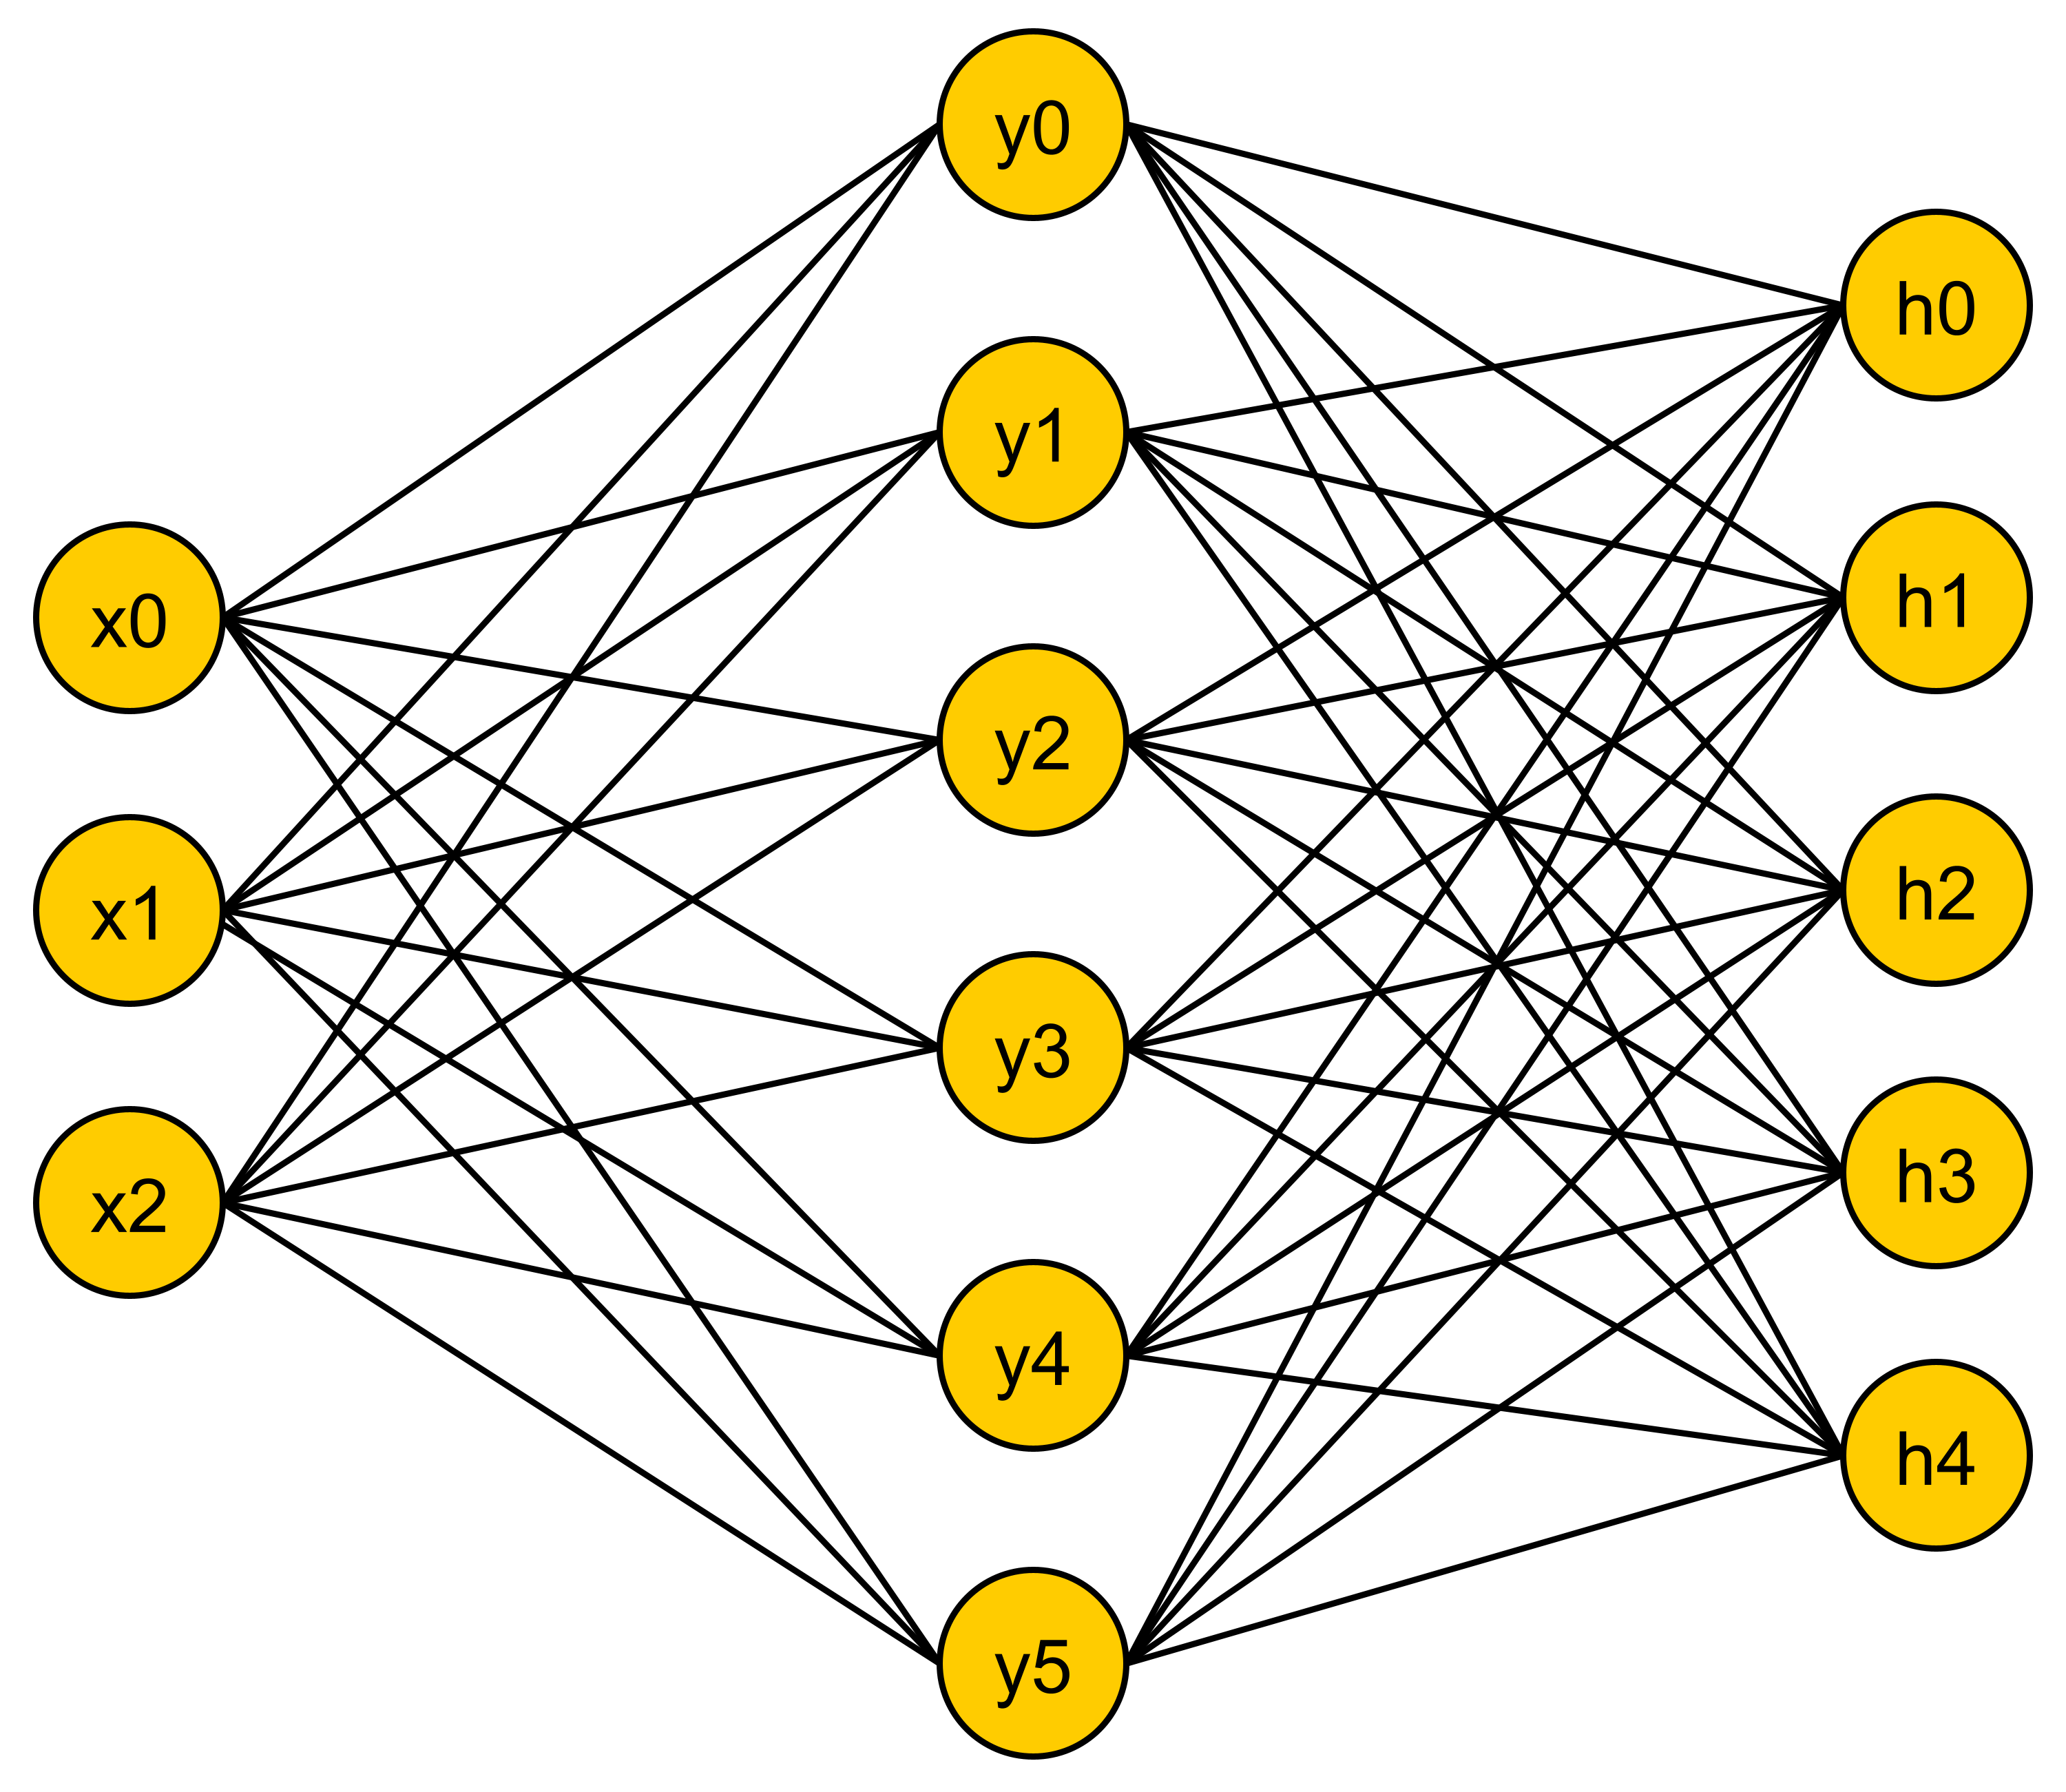
\includegraphics[scale=0.08]{img/nn_enemy_character.png}
	\caption{Arsitektur \textit{Neural Network} untuk klasifikasi karakter musuh.}
	\label{fig:nn_enemy}
	\vspace{1ex}
\end{figure}

Misalkan model kita 100\% yakin jika karakter A adalah \textit{Hard Strength}, maka keluaran dari model adalah $\left[1,\ 0,\ 0,\ 0,\ 0 \right]$ dan jika model kita 50\% yakin jika hero B adalah \textit{Soft Strength}, 25\% yakin jika hero B adalah \textit{Hard Strength} atau \textit{Hard Magic}, maka keluaran dari model ini adalah $\left[0.25,\ 0.5,\ 0.25, \ 0, \ 0 \right]$. Harus diingat bahwa total nilai dari distribusi probabilitas untuk semua target adalah 1.
\vspace{1ex}

Sedangkan untuk \textit{loss function} yang digunakan adalah \textit{Cross Entropy} dan \textit{Optimizer} yang digunakan adalah SGD (\textit{Stochasstic Gradient Descent}) dengan \textit{learning rate} sebesar 0.001. Sebagai catatan penambahkan \textit{metrics accuracy} bertujuan untuk melihat seberapa bagus model ini dalam melakukan klasifikasi.
\vspace{1ex}

\subsection{Training dan Pembuatan Model}
\label{sec:sub_sec3_enemy_char_train}
\vspace{1ex}

Data hasil dari korelasi fitur pada Sub-bab \ref{sec:sub_sec3_enemy_feature_corel}, karena tipe yang ditunjukan pada kolom ke satu dengan kepala bertuliskan ``Fitur'' adalah pedoman hasil prediksi maka tidak akan diikutkan proses \textit{training}. Pada kolom \textit{type} tipe karakter dinyatakan dengan 0, 1, 2, 3, dan 4 yang menyatakan \textit{Mixed}, \textit{Hard Strength}, \textit{Soft Strength}, \textit{Hard Magic} dan \textit{Soft Magic}. Nantinya keluaran dari hasil \textit{training} yang menunjukan prediksi tipe dari karakter dinyatakan dalam bentuk \textit{one-hot vector}: \textit{Mixed} $\rightarrow [1, 0, 0, 0, 0]$, \textit{Hard Strength} $\rightarrow [0, 1, 0, 0, 0]$, \textit{Soft Strength} $\rightarrow [0, 0, 1, 0, 0]$, \textit{Hard Magic} $\rightarrow [0, 0, 0, 1, 0]$, dan \textit{Soft Magic} $\rightarrow [0, 0, 0, 0, 1]$. Kemudian untuk optimasi dan pembuatan model sama seperti Sub-bab \ref{sec:sub_sec3_dota2_model}. Model yang dihasilkan dari proses \textit{training} pada Sub-bab \ref{sec:sub_sec3_enemy_char_train} dapat digunakan untuk menguji atau menampilkan hasil klasifikasi pada data testing yang dibahas pada Sub-bab \ref{sec:sec4_eval_dota2}.
\vspace{1ex}